\chapter{Sensing Platform} \label{sensing_platform}


        

%%%%%%%%%%%%%%%%%
% \subsection{Livox LiDAR} \label{sensors_LiDAR}

% The Minion platform features six \ac{LiDAR} units providing both omnidirectional environmental awareness and forward-facing high-density perception.
% The \ac{LiDAR} suite comprises three Velodyne HDL-32E units and three Livox Horizon units.

% The three Velodyne HDL-32E mechanically rotating 360-degree \ac{LiDAR} sensors are positioned to provide complete omnidirectional point cloud coverage.
% One unit is positioned at aft-center, with the other two placed at approximately one-third intervals around the vessel at forward-port and forward-starboard locations to achieve a full 360-degree \ac{FOV} coverage.

% The three Livox Horizon solid-state forward-scanning \ac{LiDAR} sensors provide high-density returns within a 165-degree forward \ac{FOV} matching the camera array coverage.
% These sensors were selected specifically for \ac{LiDAR}-camera fusion research based on superior point cloud density within the camera \ac{FOV} and a non-repetitive scan pattern that enhances coverage through temporal aggregation \cite{thompson2023}.

% While 360-degree coverage provides comprehensive spatial awareness, it presents challenges for camera-\ac{LiDAR} fusion.
% First, sparse azimuthal sampling occurs because on a stationary or slow-moving platform, the 32 lasers strike identical positions on every rotation, yielding no increase in sampling density over time.
% Second, inefficient \ac{FOV} utilization results from distributing returns across 360 degrees, such that only a fraction falls within the forward-facing camera view.
% These limitations motivated the selection of an alternative \ac{LiDAR} technology optimized for forward-facing perception with temporal aggregation.

% The Livox Horizon employs a non-repetitive rosette scan pattern that progressively covers its \ac{FOV} over time rather than repeatedly sampling identical locations.
% The sensor features an 81.7-degree × 25.1-degree (horizontal × vertical) \ac{FOV}, substantially wider in azimuth than the 65-degree cameras.
% Three Livox units deployed together achieve a combined coverage of approximately 165 × 25.1 degrees, providing complete horizontal overlap with the camera array and covering approximately 77\% vertically \cite{thompson2023}.
% Table 3.2 presents the Livox Horizon specifications.

% \begin{table}[htpb]
% \centering
% \caption{LiDAR Specifications}
% \begin{tabular}{ll}
% \hline
% \multicolumn{2}{c}{Livox Horizon}\\
% \hline
% % \textbf{Parameter} & \textbf{Value} \\
% \hline
% Model & Livox Horizon \\
% Horizontal Field of View & 81.7 degree \\
% Vertical Field of View & 25.1 degree \\
% Range & 260 m @ 80\% reflectivity \\
% Point Rate (Single Return) & 240,000 pts/sec \\
% Point Rate (Dual Return) & 480,000 pts/sec \\
% Range Precision & ±2 cm \\
% Wavelength & 905 nm \\
% Scan Pattern & Non-repetitive rosette \\
% Interface & Ethernet \\
% Operating Frequency & 100 Hz \\
% \hline
% \end{tabular}
% \label{tab:livox_horizon_specs}
% \end{table}



% The non-repetitive scan pattern demonstrates particular advantage when aggregating multiple scans over time, accumulating points over an integration window to enhance spatial sampling.
% On a moving platform, motion compensation during the accumulation period becomes necessary.
% The \ac{LiDAR} aggregation approach, detailed in Chapter 5, employs the \ac{GPS}/\ac{IMU} to track platform pose over time.
% Each \ac{LiDAR} point is transformed from sensor coordinates to a world reference frame using the platform pose at that point's timestamp.
% All accumulated points are then transformed from world coordinates to the target camera image frame, enabling overlay of a dense point cloud on the image.
% A four-second integration period was selected based on empirical evaluation of the tradeoff between point cloud density and motion blur.
% Each camera image sampled at 1 Hz receives all \ac{LiDAR} points from the preceding four seconds, transformed to the image capture time.
% This approach provides the spatial resolution necessary for reliable detection while maintaining sufficient motion compensation accuracy for typical vessel speeds.

% The Livox Horizon sensors communicate via \ac{UDP} over Ethernet, transmitting point cloud data as binary messages at 100 Hz.
% Livox provides an open-source \ac{ROS} SDK that manages network communication, message parsing, and point cloud publication to \ac{ROS} topics.
% Integration of the Livox SDK into the Minion software required minimal effort, primarily involving network configuration and modification of \ac{ROS} launch files.
% The SDK operates on the Atlas PC, receiving \ac{UDP} messages from all three \ac{LiDAR} units simultaneously over the local network described in Section 3.1.2.3.

% Accurate fusion of data from multiple \ac{LiDAR} units requires precise knowledge of sensor geometric relationships.
% The Livox Horizon units feature onboard storage for extrinsic calibration parameters, enabling each sensor to transform its measurements to a common reference frame before transmission.
% The \ac{LiDAR}-to-\ac{LiDAR} extrinsic calibration presented in Section 3.2.1.3 determines the six-degree-of-freedom transformation (translation and rotation) relating each sensor's local coordinates to the designated primary sensor.
% These parameters are written to non-volatile memory on each Livox unit, configuring automatic application of the transformation such that all point clouds emerge in the center \ac{LiDAR}'s reference frame \cite{thompson2023}.
% This onboard configuration simplifies downstream processing by eliminating the need for software-based registration of the three point clouds.
% The unified cloud is subsequently related to camera coordinates through camera-to-\ac{LiDAR} extrinsic calibration described in Section 3.2.1.2.

% Temporal alignment of \ac{LiDAR} with camera images and \ac{GPS}/\ac{IMU} pose requires all \ac{LiDAR} points to possess timestamps referenced to a common global time base.
% The Livox Horizon supports IEEE 1588 Precision Time Protocol, providing sub-microsecond clock synchronization with a \ac{PTP} master on the network.
% In this configuration, the NVIDIA Jetson Xavier in the camera box functions as the \ac{PTP} master, synchronizing the three \ac{LiDAR} units.
% The Jetson itself synchronizes to \ac{GPS} time via the Network Time Protocol hierarchy detailed in Section 3.2.2.1.
% This cascaded synchronization ensures \ac{LiDAR} timestamps share the same \ac{GPS}-disciplined time reference as camera frames, enabling frame-accurate alignment for fusion.
% \ac{PTP} synchronization status is verified using the Livox Viewer software, which displays sync state and time source for each sensor.
% Proper \ac{PTP} lock is confirmed prior to data collection, ensuring timestamp accuracy.

% An advantageous characteristic of the 905 nm wavelength is its strong absorption by water.
% This results in minimal \ac{LiDAR} returns from water surfaces, contrasting with vision sensors that clearly image water texture and waves.
% Absence of water returns reduces point cloud clutter and simplifies object detection by eliminating the need to filter ground plane points for the water surface.
% Point cloud visualizations overlaid on camera images demonstrate this characteristic: dense \ac{LiDAR} coverage appears on vessels, buoys, and other solid objects, while water surfaces produce few or no returns.
% For grid-based clustering, this characteristic prevents false positives from wave crests or foam patterns.

% The Livox Horizon configuration provides several capabilities essential for comparing object detection performance.
% The system achieves 2.25× more points within the camera view compared to omnidirectional spinning sensors, while the non-repetitive scan pattern enhances sampling density through temporal aggregation.
% Per-point timestamps and \ac{GPS}/\ac{IMU} integration enable accurate aggregation during motion, while \ac{PTP} synchronization provides sub-microsecond timing accuracy relative to cameras and \ac{GPS}.
% Factory-configured multi-sensor calibration unifies point clouds from three sensors before transmission, and the 905 nm wavelength reduces maritime clutter by rejecting water returns.
% Combined with the software integration and synchronization infrastructure described in Section 3.2, this configuration enables rigorous \ac{LiDAR} detection evaluation and comparison with vision-based approaches in Chapters 5 and 6.

%%%%%%%%%%%%%%%%%%
\subsection{LiDAR Systems} \label{sensors_LiDAR}

The Minion platform features six \ac{LiDAR} units providing both omnidirectional environmental awareness and forward-facing high-density perception.
The \ac{LiDAR} suite comprises three Velodyne HDL-32E units and three Livox Horizon units.

The three Velodyne HDL-32E mechanically rotating 360-degree \ac{LiDAR} sensors are positioned at aft-center, with the other two placed at approximately one-third intervals around the vessel at forward-port and forward-starboard locations to achieve full 360-degree \ac{FOV} coverage.
These sensors provide the spatial awareness necessary for autonomous navigation and collision avoidance.

The three Livox Horizon forward-scanning \ac{LiDAR} sensors provide high-density returns within the camera's \ac{FOV} and serve as the primary \ac{LiDAR} sensors for this research.
While the Velodyne units provide adequate omnidirectional awareness for navigation, they present fundamental limitations for camera-\ac{LiDAR} fusion research.

% MOTIVATION - Why Livox over Velodyne
LiDAR sensors with fixed 360-degree scan patterns, such as the Velodyne HDL-32E, impose limitations on object-detection research.
Because the scan maintains a constant elevation and azimuth with each rotation, the sensor repeatedly samples the same positions, resulting in a sparse representation of objects with a low relative velocity to the sensor.
This parallels the resolution of optical cameras; lower density returns limit the ability to resolve features on small or distant objects, as the sparsity increases linearly with range.

The Livox Horizon addresses this limitation through a fundamentally different scan architecture.
Rather than repeatedly sampling fixed positions, the sensor employs a non-repetitive rosette scan pattern that progressively covers its \ac{FOV} over time, as visualized in Figure \ref{fig:livox_scan_pattern}.
This irregular sampling pattern produces substantially denser point cloud data, critical for the object detection methods described in Section \ref{gbcache}, and motivated their selection for the forward-scanning perception suite \cite{thompson2023}.


Each Livox Horizon sensor features an 81.7-degree (horizontal)\ac{FOV} and are mounted to provide more than 50\% overlap between units.
This configuration effectively doubles the number of returned points within the 65-degree \ac{FOV} of the primary forward camera and creates a system that is robust to individual sensor failure.
Table~\ref{tab:livox_horizon_specs} presents the Livox Horizon specifications.

\begin{table}[htpb]
\centering
\caption{LiDAR Specifications}
\begin{tabular}{ll}
\hline
\multicolumn{2}{c}{Livox Horizon}\\
\hline
% \textbf{Parameter} & \textbf{Value} \\
\hline
Model & Livox Horizon \\
Horizontal Field of View & 81.7 degree \\
Vertical Field of View & 25.1 degree \\
Range & 260 m @ 80\% reflectivity \\
Point Rate (Single Return) & 240,000 pts/sec \\
Point Rate (Dual Return) & 480,000 pts/sec \\
Range Precision & ±2 cm \\
Wavelength & 905 nm \\
Scan Pattern & Non-repetitive rosette \\
Interface & Ethernet \\
Operating Frequency & 100 Hz \\
\hline
\end{tabular}
\label{tab:livox_horizon_specs}
\end{table}

\begin{figure}[htbp]
\centering
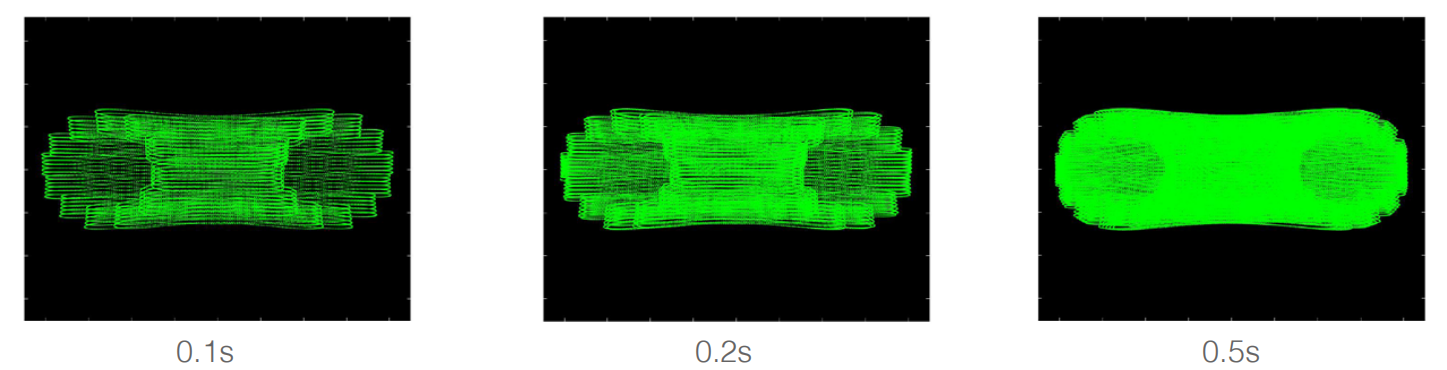
\includegraphics[width=0.8\textwidth]{Images/Livox_1.png}
\caption{Livox Horizon non-repetitive rosette scan pattern demonstrating point cloud density distribution from 0.1 to 0.5 seconds.}
\label{fig:livox_scan_pattern}
\end{figure}

% The sensor employs a two-dimensional scanning mechanism that traces a non-repetitive rosette pattern across the \ac{FOV}.
The sensor employs two orthogonal mirrors operating at slightly different frequencies to trace a complex Lissajous-like path that progressively fills the \ac{FOV} without repetition at a maximum rate of $480000$ points per second per device.
\textcolor{red}{cite Livox documentation?}.

The Livox Horizon sensors communicate via \ac{UDP} over Ethernet, transmitting point cloud data as binary messages at 100 Hz.
Each point consists of position coordinates (x, y, z), intensity, and timestamp, totaling 16 bytes per point.
At maximum point rate (480,000 pts/sec per sensor), three sensors generate approximately:

$$\text{Peak bandwidth} = 3 \times 480,000 \times 16 \text{ bytes/sec} \approx 23 \text{ Mbps}$$

In practice, the sensors are configured to suppress null returns (points beyond maximum range or with insufficient reflectivity), reducing actual network traffic below this theoretical maximum.
% The rosette pattern provides substantially higher spatial coverage compared to a spinning sensor's fixed ring geometry, particularly in the vertical dimension where traditional spinning sensors are limited to discrete horizontal rings.
% This density characteristic is critical for the grid-based clustering approach employed for \ac{LiDAR} object detection in Chapter 5.

The 905 nm near-infrared wavelength experiences strong absorption by water, resulting in minimal returns from water surfaces.
This characteristic benefits maritime object detection by reducing clutter from waves that would otherwise trigger false positives in clustering algorithms.
\textcolor{red}{Figure \#} demonstrates this effect: dense \ac{LiDAR} coverage appearing on vessels, buoys, and other solid objects, while water surfaces produce few or no returns.
\textcolor{red}{insert figure to compare Velodyne and Livox returns in situ.}

% Comparison of point cloud density within the camera \ac{FOV} quantifies the Livox advantage over traditional spinning sensors.
% A Velodyne HDL-32E in dual-return mode produces approximately 1.4 million points per second distributed across the full 360-degree plane.
% The camera \ac{FOV} encompasses approximately 165 degrees, yielding an effective point rate in the region of interest of:

% $$\text{Effective HDL-32E rate} = 1.4 \times 10^6 \times \frac{165°}{360°} \approx 641,000 \text{ pts/sec}$$

% Three Livox Horizon units in dual-return mode together produce:

% $$\text{Combined Livox rate} = 3 \times 480,000 = 1.44 \times 10^6 \text{ pts/sec}$$

% This represents a 2.25× increase in point returns within the camera view, excluding additional benefits from superior vertical sampling achieved through the non-repetitive pattern compared to fixed 32-ring geometry \cite{thompson2023}.



% Accurate fusion of data from multiple \ac{LiDAR} units requires precise knowledge of sensor geometric relationships.
The Livox Horizon units feature onboard storage for extrinsic calibration parameters, enabling each sensor to transform its measurements to a common reference frame before transmission.
These parameters are written to non-volatile memory on each Livox unit and applied before data transmission so that all LiDAR returns are received in the center \ac{LiDAR}'s reference frame, reducing the necessary calculation further down the data pipeline.
\textcolor{red}{cite Livox documentation?}.
% enhancing their real-time operational advantage by reducing additional computation later in the pipeline.
The calibration methodology to determine these extrinsic values is detailed in Section~\ref{lidar_extrinsic}.


%%%%%%%%%%%%%%%%%%
% \subsection{LWIR Thermal Cameras} \label{sensors_LWIR}
% Two Teledyne Calibir 640 \ac{LWIR} thermal cameras extend perception to night and low-light conditions. 
% While limited to 640×480 resolution due to bolometer technology, they provide a combined 165-degree forward \ac{FOV} when paired, ensuring redundancy with the
% visible and \ac{HDR} cameras.
% \textcolor{red}{Possibly remove this subsection?}





\subsubsection{HDR Selection}

The FLIR Blackfly S 4K cameras satisfy geometric and resolution requirements, but their limited dynamic range makes them prone to over-exposure and loss of highlight detail in high-contrast maritime conditions. 
They support an effective dynamic range of 69.4~dB, which corresponds to a span of just a few thousand-to-one between the darkest detectable signal and the brightest non-saturating signal. 
As a result, the cameras are prone to over-exposure in high-brightness maritime conditions, particularly when imaging reflective water surfaces or bright sky backgrounds, leading to loss of highlight detail and reduced contrast. 

In contrast, the IMX490 \ac{HDR} camera combines a comparable \ac{FOV} with substantially greater dynamic range, enabling detail preservation across bright and shaded regions within the same frame.  
For these reasons, the \ac{HDR} camera was designated as the primary forward-facing visual spectrum sensor for \ac{LiDAR}-camera fusion research.  
 
As a result, the cameras are prone to over-exposure in high-brightness maritime conditions, particularly when imaging reflective water surfaces or bright sky backgrounds, leading to loss of highlight detail and reduced contrast.  



        




\subsection{Sensor Transforms}
The multi-sensor system aboard the WAM-V requires rigorous coordinate frame transformations to fuse data from heterogeneous sensors into a unified representation. Each sensor operates in its native coordinate frame, necessitating extrinsic calibration to establish spatial relationships between sensors and the vessel's body frame.

The fundamental transformation between coordinate frames is expressed as:
\begin{equation}
^Bp =\; ^B_AR \; ^Ap + ^B_A T
\end{equation}
where points in reference frame $A$ ($^Ap$) are transformed into reference frame $B$ ($^Bp$) through a rotation matrix $^B_AR$ and translation vector $^B_A T$.

% \subsubsection{Coordinate Frame Definitions}
The selected sensors employ multiple coordinate frames, each with distinct conventions:

% \textbf{Inertial Frame (Map):} 
The global reference frame follows the North-East-Down (NED) convention, where the x-axis points north, y-axis points east, and z-axis points downward toward the earth's center. This right-handed frame provides a consistent world reference for navigation and localization.

% \textbf{LiDAR Frame:} 
The Livox Horizon sensors capture point cloud data in the Forward-Left-Up (FLU) convention, where x-axis points forward along the sensor's optical axis, y-axis points left, and z-axis points upward. Each of the three LiDAR units maintains this local frame relative to its mounting position.

% \textbf{GPS Frame:} 
The GPS receiver outputs position data in geodetic coordinates (latitude, longitude, altitude), which are converted to Cartesian coordinates in the FLU body frame using the vessel heading from the inertial measurement unit (IMU). This transformation accounts for the spherical earth geometry and local tangent plane approximation.

% \textbf{Camera Frame:} 
The Leopard Imaging camera operates in a standard image plane coordinate system where the u-axis (horizontal) points right, v-axis (vertical) points down, and the optical axis extends forward along the camera's line of sight. Image coordinates require both extrinsic transforms to the body frame and intrinsic camera calibration for 3D reconstruction.

The sensor-to-body and body-to-inertial transformations are all handled through the \Ac{ROS} robot-localization package onboard the \Acp{USV} main computer, Atlas.
%%%%%%%%%%%%%%%%%%%%%%%%%%%%%%
\begin{figure}[htbp]
\centering
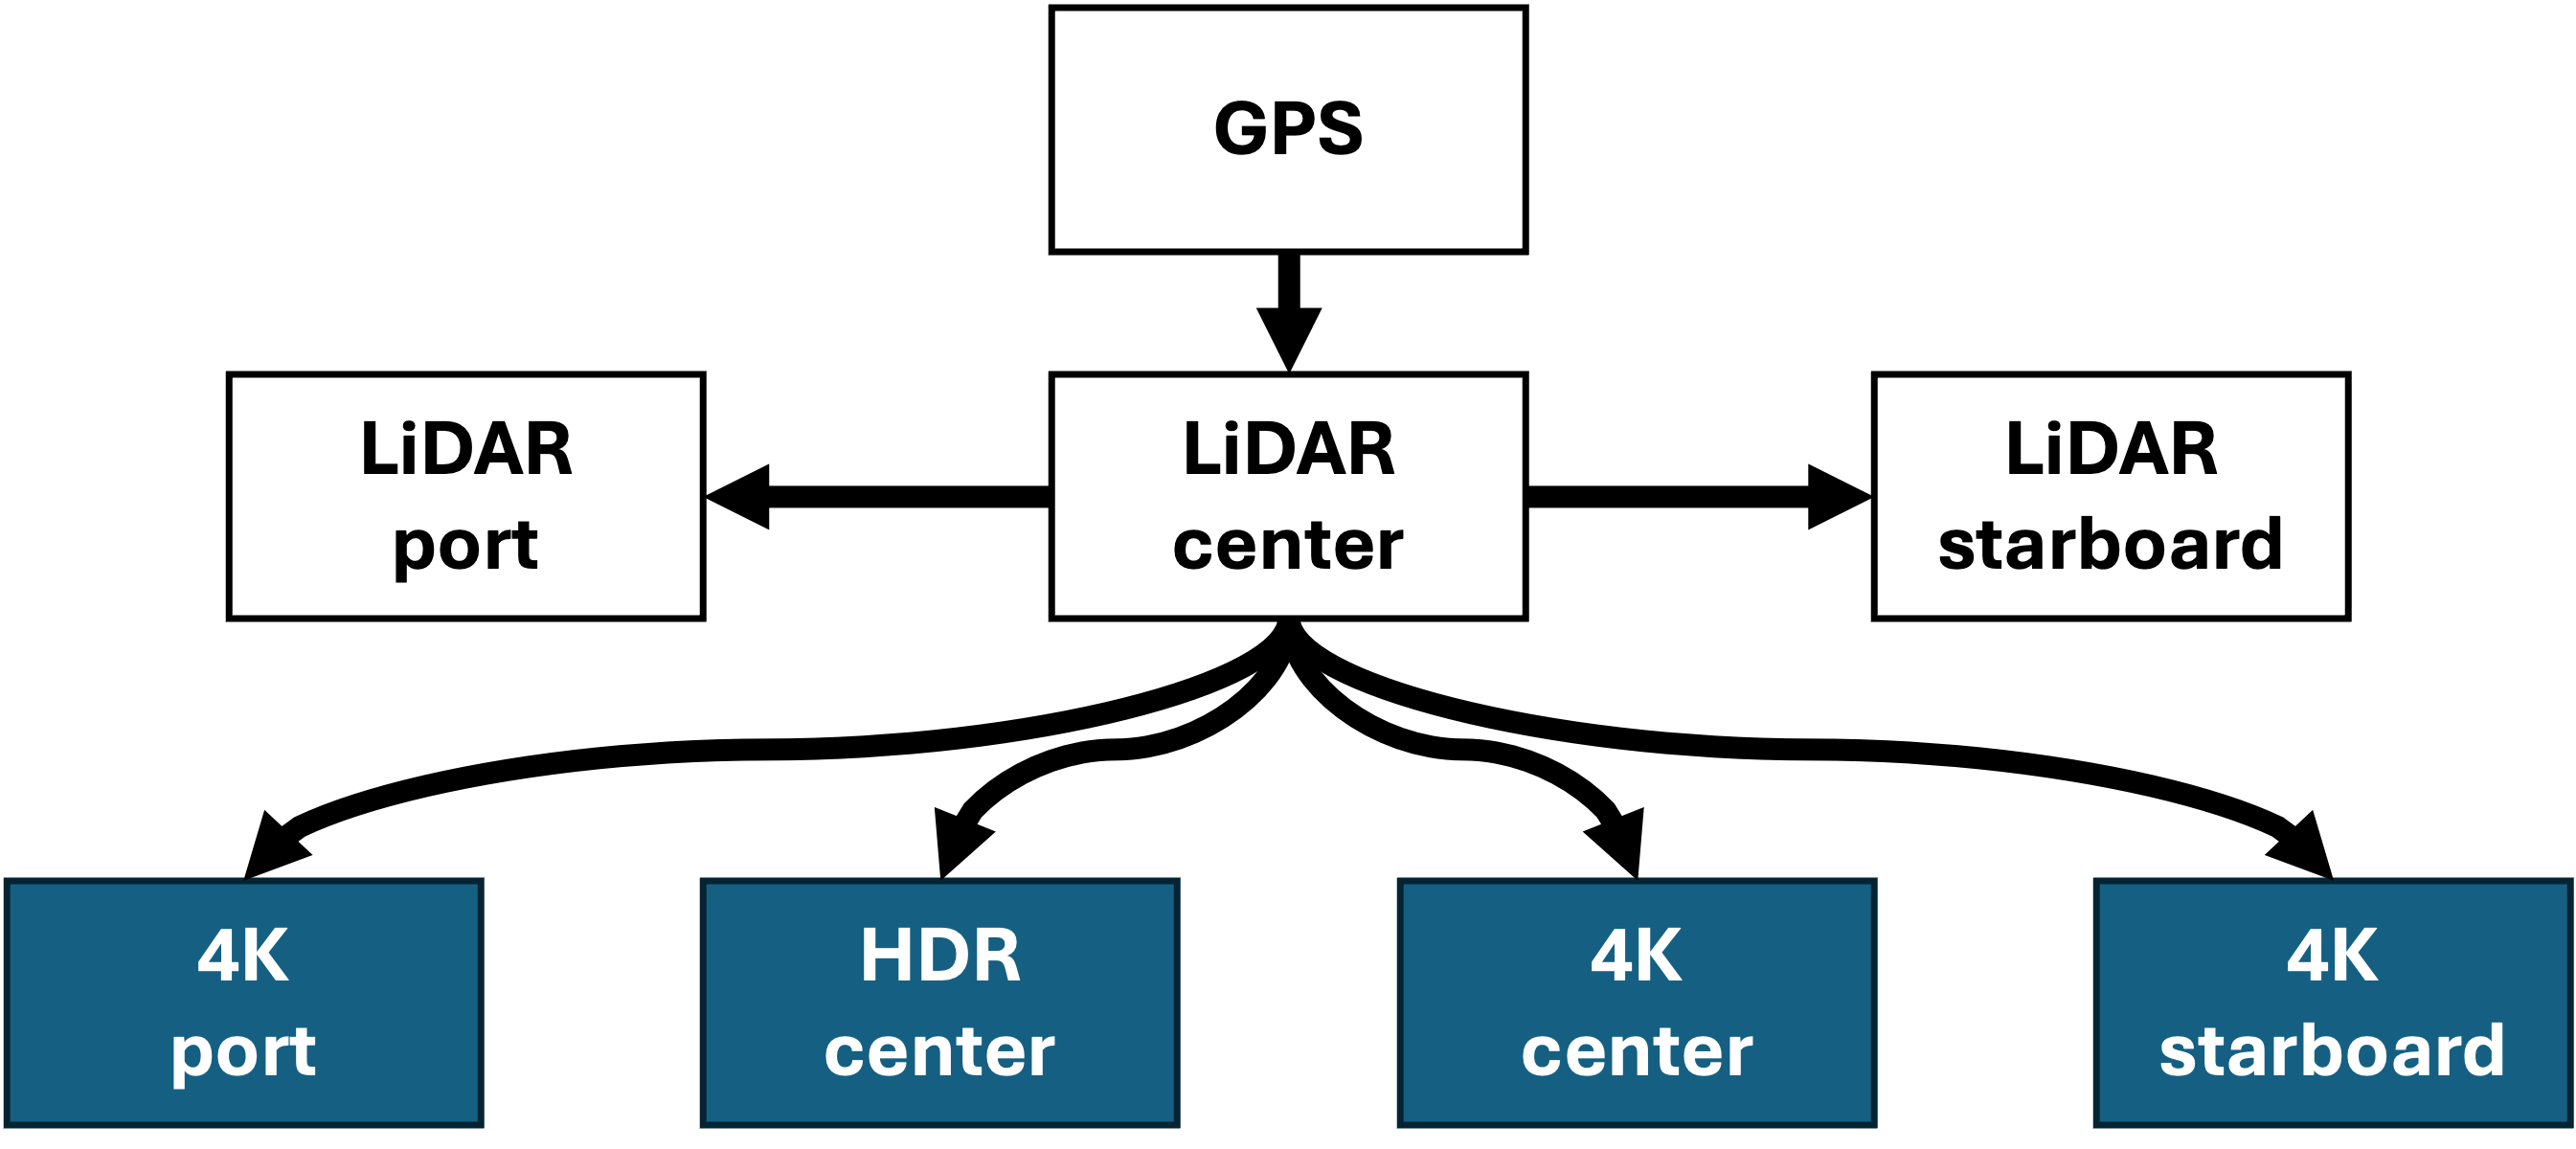
\includegraphics[width=0.75\textwidth]{Images/spatial_transforms.png}
\caption{A flowchart of transforms between sensor reference frames. Arrows indicate extrinsic transformations, and dark boxes indicate an additional intrinsic transform.}
\label{transform_diagm}
\end{figure}
%%%%%%%%%%%%%%%%%%%%%%%%%%%%%%

\section{Compute and LAN} \label{compute_lan}

The Minion platform's computing architecture consists of two primary systems: a main compute module housed in a waterproof Pelican case and a dedicated camera enclosure with integrated processing. The main compute module contains the Atlas PC and a 16-port network switch that aggregates all sensor and subsystem connections. The camera enclosure integrates a self-contained computing system responsible for camera data acquisition, video encoding, and timestamp synchronization with the vessel's global time reference. This modular architecture enables independent development and testing of the perception system while maintaining compatibility with the broader platform infrastructure.

\subsection{Camera Enclosure Computing Platform} \label{jetson_platform}

An NVIDIA Jetson AGX Xavier serves as the dedicated computer within the camera enclosure, handling all camera interface, video encoding, and network streaming operations. The Jetson was selected for its GPU acceleration capabilities, compact form factor, and native support for industrial camera interfaces including GMSL2 (Gigabit Multimedia Serial Link) required by the Leopard Imaging HDR camera.

The Jetson AGX Xavier features an 8-core ARM CPU, 512-core Volta GPU with 64 Tensor cores, and 32 GB of unified memory, providing sufficient computational resources for real-time video encoding of multiple simultaneous camera streams. The integrated GPU enables hardware-accelerated H.264/H.265 video encoding, reducing CPU load and network bandwidth requirements compared to uncompressed image transmission.

The Jetson connects directly to all cameras within the enclosure: the Leopard Imaging HDR camera via GMSL2 interface and three FLIR Blackfly S cameras via GigE Vision over Ethernet. Custom \ac{ROS} driver nodes execute on the Jetson to interface with each camera, configure acquisition parameters, capture frames, embed timestamps, encode video streams, and transmit encoded data to the vessel's main computer.

% A critical function of the Jetson platform is timestamp embedding for temporal synchronization. As described in Section~\ref{temporal_sync}, accurate sensor fusion requires camera frame timestamps to represent the actual moment of image capture referenced to a global time base. The Jetson system clock synchronizes to the vessel's \ac{GPS}-disciplined time reference via Network Time Protocol, then embeds synchronized timestamps into each video frame as supplemental encoded information (SEI) data within the H.264 stream. This approach ensures frame timestamps remain associated with image data throughout network transmission and decoding.

The camera enclosure design emphasizes modularity and research flexibility. The self-contained Jetson computer with local camera connections enables the perception system to be removed, modified, and tested independently of the Minion platform. Firmware updates, camera reconfiguration, and software development can proceed in the laboratory without requiring access to the full vessel. Network connectivity to the Minion platform occurs through a single Ethernet connection carrying both encoded video streams via \ac{RTP} and bidirectional \ac{NTP} for clock synchronization.

\subsection{Network Architecture} \label{network_structure}

% The Minion platform implements a hierarchical local area network (LAN) architecture connecting all computing resources and sensors. The network topology separates high-bandwidth sensor data streams from lower-rate command and control traffic while maintaining deterministic latency for time-critical communications.

The Atlas PC functions as the central computing node, hosting the primary \ac{ROS} environment, object detection algorithms, mission planning software, and data logging infrastructure. Atlas connects to the vessel LAN via a gigabit Ethernet switch that aggregates connections from all network-capable sensors and subsystems.

% Key network endpoints include:
% \begin{itemize}
% \item \textbf{Jetson AGX Xavier} (camera enclosure): Video streams and timestamp synchronization
% \item \textbf{Livox Horizon \ac{LiDAR} units} (3 sensors): UDP point cloud data at 100 Hz per sensor
% \item \textbf{PinPoint \ac{GPS}/\ac{IMU}}: Pose data and Network Time Protocol time reference
% \item \textbf{Velodyne HDL-32E \ac{LiDAR} units} (3 sensors): UDP point cloud data for navigation
% \item \textbf{Shore connection}: Ground station monitoring and remote access during development
% \end{itemize}

Static IP address assignment ensures deterministic routing and simplifies network administration. The PinPoint \ac{GPS}/\ac{IMU} is configured with IP address 201.7.90.30 and designated as the authoritative Network Time Protocol server for the vessel. All other computing resources synchronize to this \ac{GPS}-disciplined time source to establish a common temporal reference.

This \ac{RTP}-based approach was developed to address network latency issues observed with alternative solutions. Open-source plugins such as GStreamer-based GSCam and NVIDIA's DeepStream SDK were evaluated but found insufficient for Minion's specific requirements. The custom implementation provides granular control over video encoding parameters (resolution, frame rate, bitrate, compression method) and ensures embedded timestamps survive the encoding-transmission-decoding pipeline without modification.

Point cloud data from the three Livox Horizon \ac{LiDAR} sensors arrives as \ac{UDP} packets transmitted directly to the Minion LAN at 100 Hz per sensor. The Livox SDK executing on Atlas receives these streams, parses binary point cloud messages, and publishes data to \ac{ROS} topics for consumption by perception algorithms. 

\begin{figure}[htbp]
    \centering
    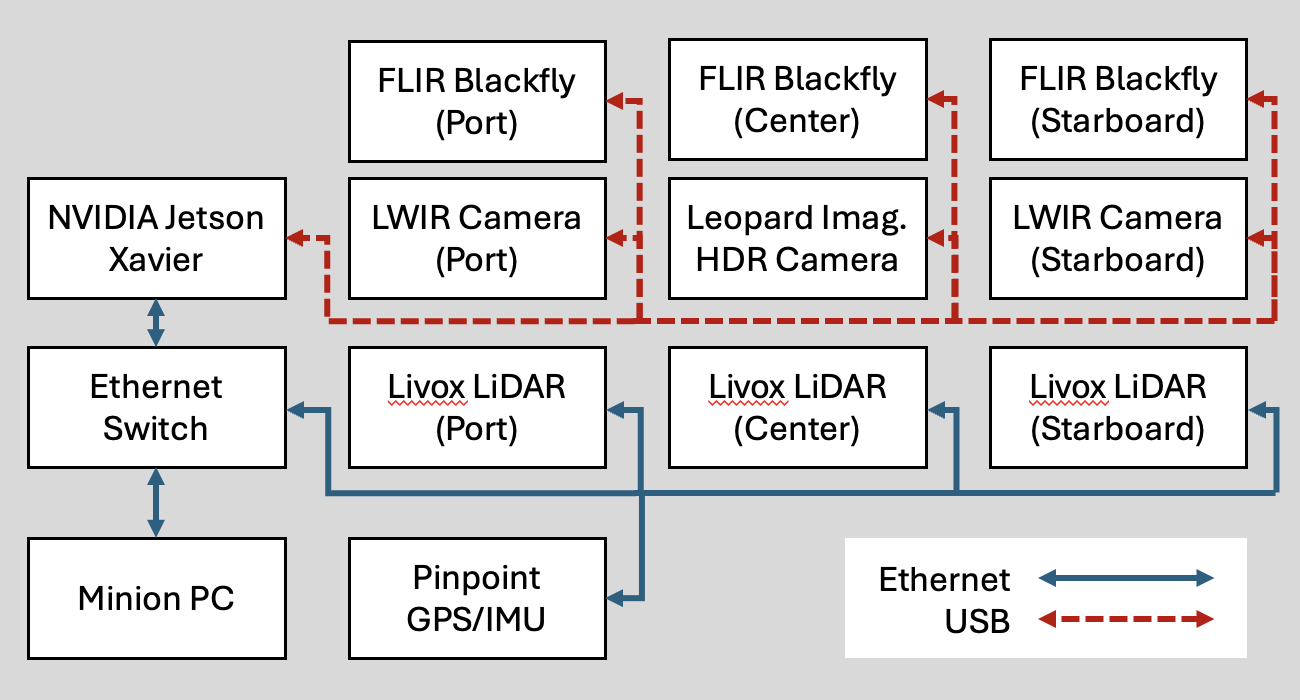
\includegraphics[width=0.85\textwidth]{Images/network_diagram.png}
    \caption{Block diagram of the network architecture of the \ac{USV}. Red dashed arrows indicate USB connections and blue solid arrows indicate Ethernet-connected blocks.}
    \label{fig:network_diag}
\end{figure}

Bandwidth analysis for the forward perception system indicates peak data rates of approximately:

\begin{table}[htbp]
\centering
\caption{Peak data rates for forward perception sensors}
\label{tab:network_bandwidth}
\begin{tabular}{lccc}
\hline
\textbf{Sensor} & \textbf{Specifications} & \textbf{Quantity} & \textbf{Data Rate} \\
\hline
Livox \ac{LiDAR} & 480k pts/sec, dual return, 100 Hz, 16 bytes/pt & 3 & $\approx$ 23 Mbps \\
HDR Camera & H.264, 5 fps, 2880$\times$1860 & 1 & 8--12 Mbps \\
% FLIR Cameras & H.264, 31 fps, 4000$\times$3000 & 3 & 15--25 Mbps each \\
\hline
\end{tabular}
\end{table}

Total sustained network load during perception operations remains well below the gigabit Ethernet capacity, ensuring minimal packet loss and deterministic latency.

Quality of Service (QoS) configuration prioritizes time-sensitive traffic such as \ac{GPS}/\ac{IMU} pose updates and Network Time Protocol synchronization packets over bulk data transfers. This ensures clock synchronization accuracy is maintained even during periods of high sensor data throughput.

The hierarchical network architecture with segregated sensor and control traffic, static addressing for deterministic routing, and low-latency \ac{UDP}-based protocols establishes a robust foundation for real-time multi-modal perception and autonomous operation.

\section{Data Collection}

Integrating the spatial precision of LiDAR data and the dense pattern information and color discernment of camera data can facilitate a much more accurate interpretation of the system environment. However, to fuse data from both modalities, these sensors must be calibrated through geometric transforms and have their measurement timing synchronized. This ensures that anything in view of either sensor can be easily cross-referenced by the other for additional information.
    
\subsection{Calibration}

First, this process entailed precise intrinsic and extrinsic calibrations to reduce the geometric error between the LiDAR and camera reference frames. 
Second, custom software was written to stream the video data to overcome network latency issues and achieve the levels of temporal accuracy required. 
This software encodes the system time that each frame is captured into the video data, which is then streamed using the \ac{RTP} from the camera enclosure to Minion's main CPU. 
On Minion, the video stream is decoded, and the image frame and embedded timestamp are published as a Robotic Operating System (ROS) message. 
These enhancements enable the accurate fusion of information between camera and LiDAR sensors at a frame rate of 5 fps.

Before the data from the camera and LiDAR sensors can be combined, each device needs to be spatially calibrated through extrinsic and intrinsic transforms. 
This ensures that the scale and position of objects seen by either sensor type can be placed into a common reference frame. 
Additionally, the data received from each device should agree upon what moment in time the data represents. 
Prior to this year's competition, latency in the video signal was compensated for by adjusting its timestamp with a constant offset, and while this method was sufficient when the USV was stationary, it created significant errors during rapid motion, especially turning.

\subsubsection{Camera Intrinsics}

Camera intrinsics refer to a camera's unique properties which define the path of light through its optical path.
These properties can functionally define the path of any ray of light through the camera lens to the exact location on the camera sensor and provide a geometric translation from a position in the 3-dimensional camera frame to a 2-dimensional pixel location in the image frame. 
It is generally represented as a $3 \times 3$ matrix as:
$$
\begin{bmatrix}
    f_x & s & c_x \\
    0 & f_y & c_y \\
    0 & 0 & 1
\end{bmatrix}
$$
where $(f_x, f_y)$ is the focal length of the camera lens in pixels, $(c_x, c_y)$ is the $(x,y)$ position (measured in pixels) in the image frame that is centered in the optical path, known as the principal point, and skew $s$ is the angle between the vertical and horizontal axis of the image frame that is generally assumed to be $s = 0$. 
Radial distortion is the spherical abortion caused by the camera lens and is represented as either one, two, or three constants of a polynomial $k_1,k_2,k_3$, where:
\begin{align*}
x_{distorted} & = x(1+k_1r^2+k_2r^4+k_3r^6)\\
y_{distorted} & = y(1+k_1r^2+k_2r^4+k_3r^6)\\
r^2 & = x^2+y^2
\end{align*}

While these values are generally published as part of the camera specifications, calibration is still required to account for manufacturing tolerances. A common method to perform this calibration is through homography, and involves capturing several images of a checkerboard pattern in multiple positions within the image frame \textcolor{blue}{The MathWorks, Inc. (2024). MATLAB version: 24.1.0 (R2024b)}.

MATLAB's Camera Calibration application uses an algorithm based on this technique, which identifies intersecting points made by the checkerboard squares and the measured distance in pixels. 
This information is cross-referenced with the physical dimensions of the checkerboard.
This tool estimates the camera's intrinsic properties by minimizing the error between the observed checkerboard patterns and projected points through a pin-hole camera model \textcolor{blue}{The MathWorks, Inc. (2024). Computer Vision Toolbox version: 24.1 (R2024a)}.
However, the accuracy of this method is dependent on the quality of the calibration data used. 
Minion's calibration dataset consisted of 23 instances of simultaneous LiDARscans and camera recordings with the checkerboard placed at various locations and distances within each camera's view. 
While only only data from the camera sensors are required to calibrate intrinsics, the LiDAR data is captured simultaneously for extrinsic calibration.
A composite of several images taken during Minion's camera calibration is provided in figure \ref{fig:camera_calib}.

\begin{figure}[htbp]
\centering
\begin{subfigure}[t]{0.45\textwidth}
    \centering
    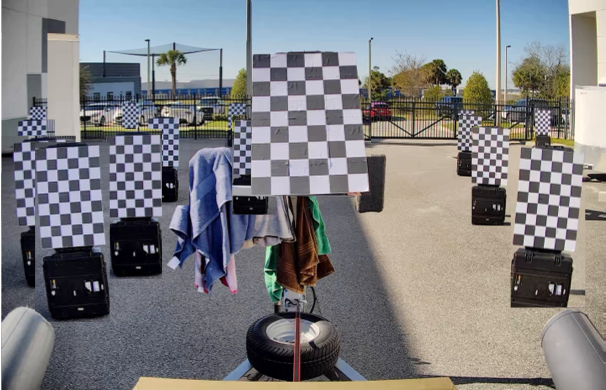
\includegraphics[width=\textwidth]{Images/checkerboard.png}
    \caption{Composite image of checkerboard locations during calibration as seen by the HDR camera}
    \label{fig:chkrbds_vision}
\end{subfigure}
\hfill
\begin{subfigure}[t]{0.45\textwidth}
    \centering
    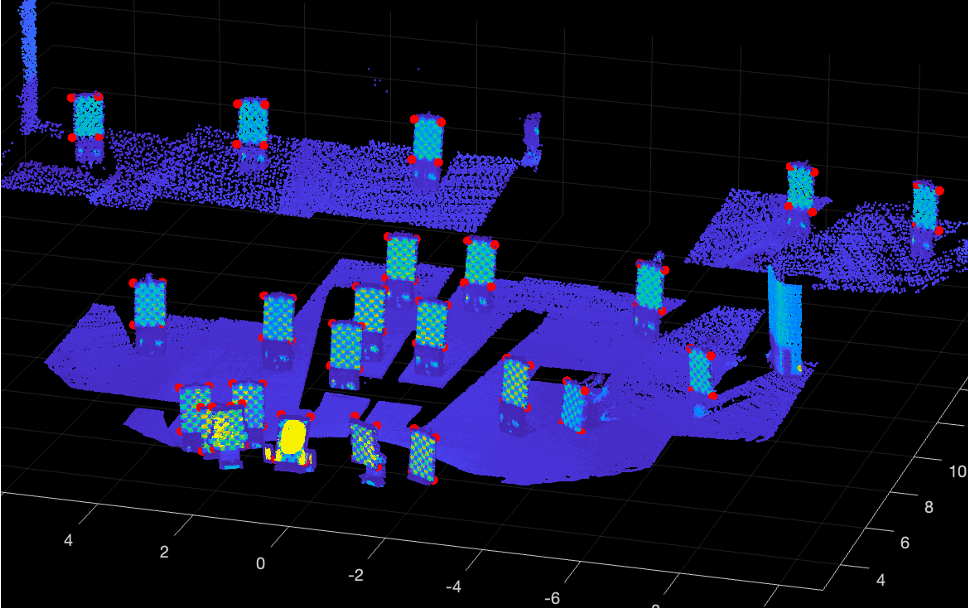
\includegraphics[width=\textwidth]{Images/lidar_calib.png}
    \caption{Composite image of the same checkerboard locations as seen by LiDAR}
    \label{fig:chkrbds_lidar}
\end{subfigure}
\caption{Comparative visualization of checkerboard co-location as seen by visual and LiDAR modality}
\label{fig:camera_calib}
\end{figure}

\begin{figure}[htbp]
    \centering
    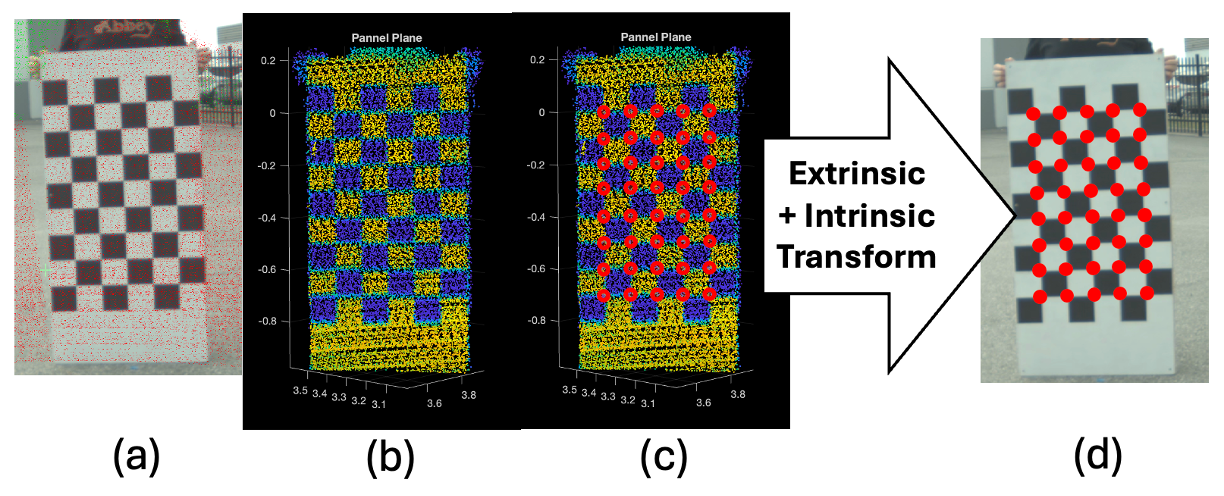
\includegraphics[width=0.9\textwidth]{Images/transform.png}
    \caption{caption}
    \label{fig:lidar_cam_calibration}
\end{figure}

            
\subsubsection{Camera Extrinsics}

For camera-to-LiDAR calibration, the checkerboard calibration dataset is reused from the camera intrinsic calibration.
One second of LiDAR scan data is isolated for each position of the checkerboard pattern to obtain a more dense point cloud and then loaded into the LiDAR Calibration tool within MATLAB.
% Data from sensor pairs (e.g. the port viewing LiDAR is paired with the port viewing 4k camera, and the center LiDAR is paired with center 4k and center HDR cameras) are loaded into MATLAB using the LiDAR Calibration application.
This function co-locates the three-dimensional checkerboard pattern from the image frame using the identified camera intrinsics and the point cloud data and then estimates the transform between them. 
This function identifies the inner corners of the checkerboard, co-locates this information in the camera and LiDAR frames, and estimates the transform between them \textcolor{blue}{The MathWorks, Inc. (2024). Computer Vision Toolbox version: 24.1 (R2024a)}. 
This initial calibration is shown in Figure \ref{fig:lidar_cam_calibration} by projecting the inner checkerboard corners detected in the images (red) into the LiDAR point cloud data.
While imperfect, this process provides a good first estimate of the extrinsic transformation between the HDR camera frame and LiDAR sensor frame.

\begin{figure}[htbp]
    \centering
    \begin{subfigure}{0.85\textwidth}
        \centering
        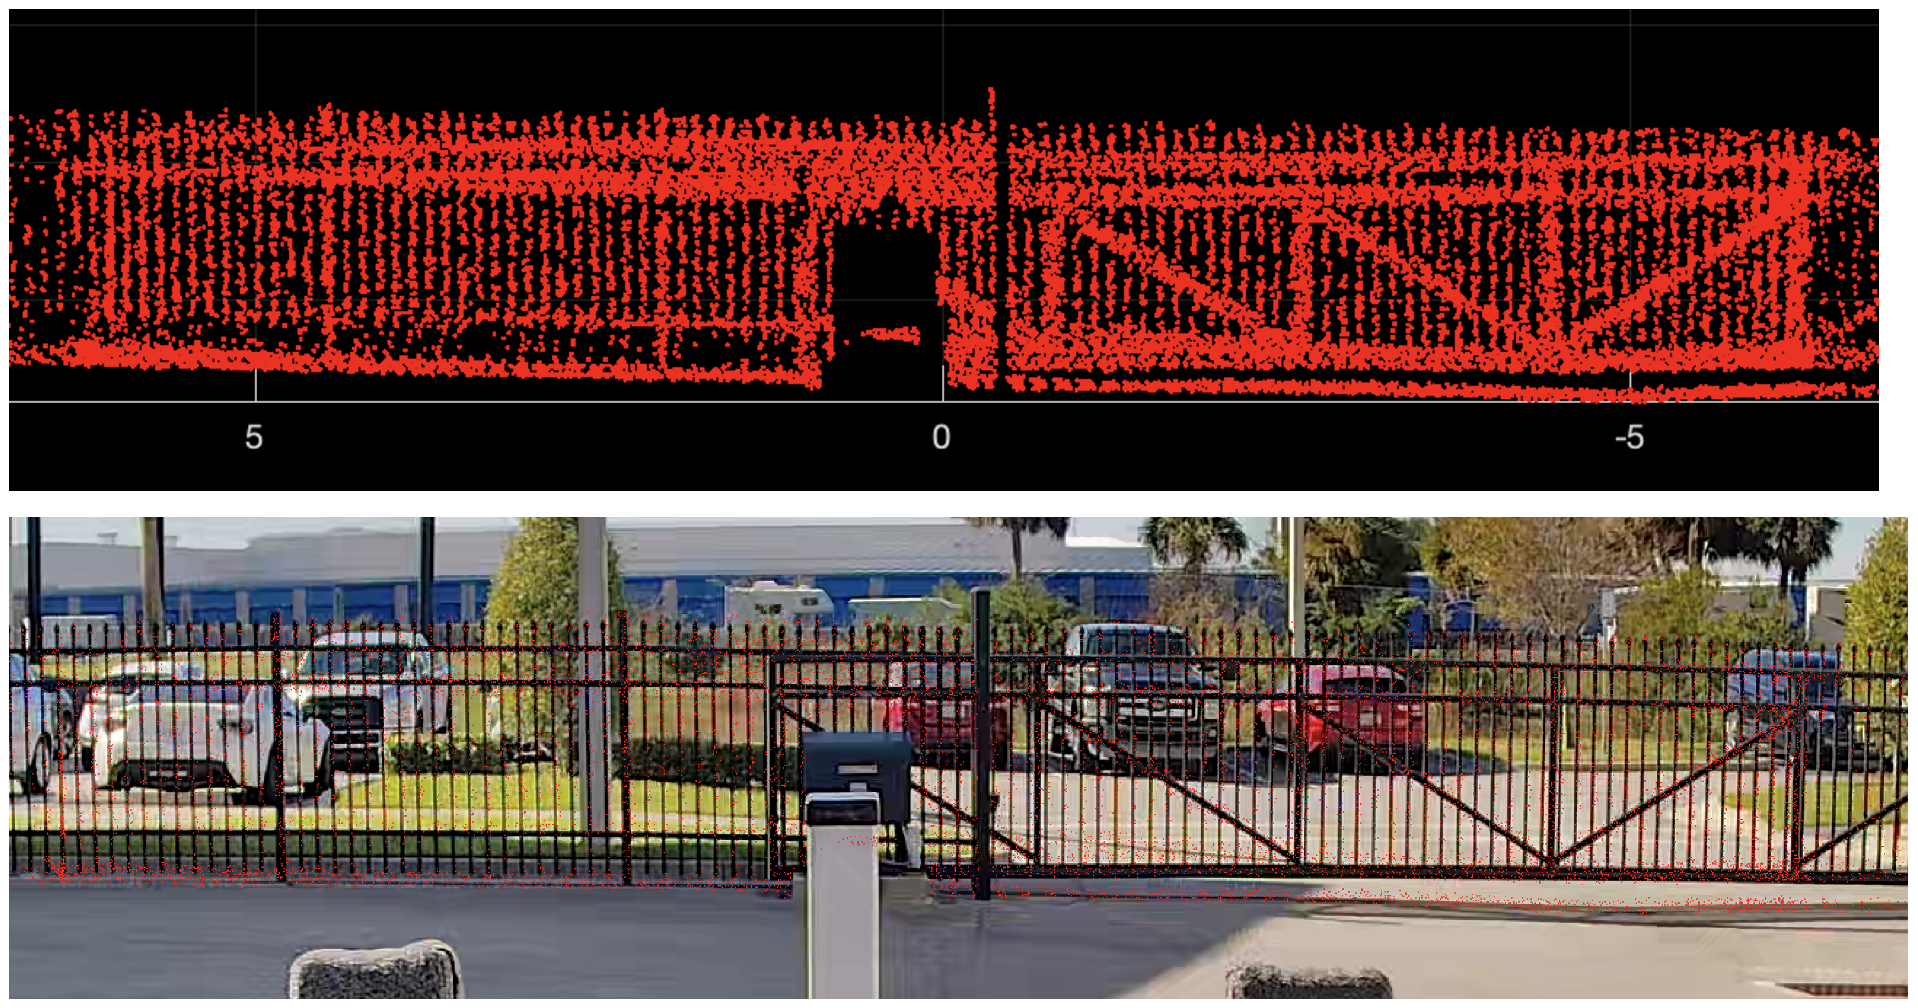
\includegraphics[width=\textwidth]{Images/LiDAR_calib_fence.png}
        \caption{Isolated LiDAR points of fencing (top) projected as red pixels onto the image frame (bottom).}
        \label{fig:LiDAR_calib_fence}
    \end{subfigure}
    
    \vspace{0.5em} % small vertical space between images

    \begin{subfigure}{0.85\textwidth}
        \centering
        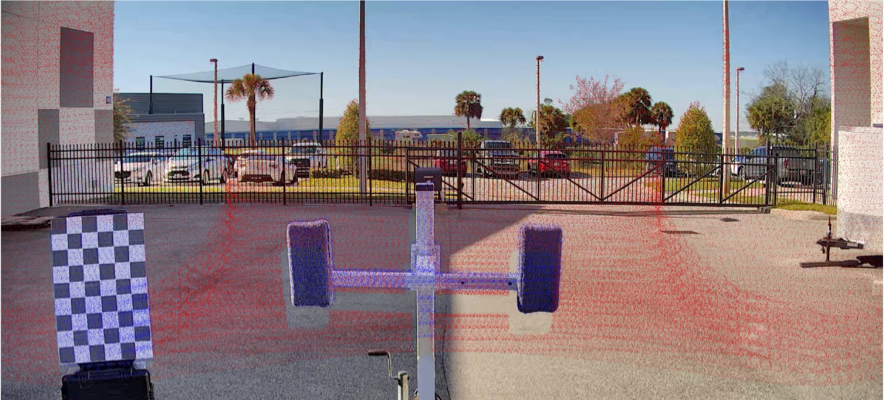
\includegraphics[width=\textwidth]{Images/LiDAR_calib_composite.png}
        \caption{LiDAR points projected onto the image frame as red pixels, with isolated foreground object points in blue}
        \label{fig:LiDAR_calib_composite}
    \end{subfigure}

    \caption{Manual refinement of Camera to LiDAR frame extrinsic transform evaluated by aligning isolated object points within the image frame.}
    \label{fig:LiDAR_calib_combined}
\end{figure}

These initial values are refined through a manual process by projecting LiDAR data onto the image frame and inspecting how the LiDAR points align with objects within the \ac{FOV} such as walls, trees, fencing, and lamp posts, as shown in Figures~\ref{fig:LiDAR_calib_fence} and~\ref{fig:LiDAR_calib_composite}.
The final extrinsic transform is provided in Table~\ref{tbl:extrinsic}.

            
\subsubsection{Livox Extrinsics} \label{lidar_extrinsic}
To identify object positions in a different reference frame than it is measured requires an extrinsic transform between the frames. 
This transform defines the translation and rotation (yaw, pitch, roll, $x,y,z$) to make one frame match another and is represented by quaternions or Euler angles.
For Minion, an extrinsic transform is used between the port and starboard facing Livox devices to the central forward facing Livox to create a unified point cloud. Each camera also receives an extrinsic transform to the Livox reference frame.
A flowchart of these transforms is provided in Figure \ref{transform_diagm}.
% required between the center Livox frame and each of the four camera sensors as well as the port and starboard Livox devices.
% Each sensor is calibrated to an $x$-up, $z$-forward, $z$-down reference frame located at the origin of the forward-facing center Livox Horizon, see \ref{transform_diagm}. 

% Each Livox Horizon is equipped with a inertial measurement unit (IMU) to ensure that the final reference frame is level.

% A similar 
% A series of LiDAR scans are simultaneously captured with video from each camera.
% Objects are accurately located within the data sets of both sensor types to perform the spatial calibration between them.

LiDAR-to-LiDAR calibration is performed with first-party software Livox Viewer, available through the manufacturer's website.
This software provides a real-time view of the LiDAR returns and adjustment of the extrinsic calibration for each sensor.
The large flat surfaces of the laboratory, as well as the larger paved area behind the laboratory, both provide excellent large and flat surfaces that allow them to be easily co-located by manually adjusting the extrinsic values.
As shown in Figure~\ref{transform_diagm}, the port and starboard Livox Horizons are transformed into the \textcolor{blue}{center livox} frame, and the extrinsic transforms required to do so are stored in the non-volatile memory of each sensor. This means that once calibrated, the raw point cloud data from each sensor is transmitted in the \textcolor{blue}{center livox} frame.




\begin{table}[ht]
\caption{Final Transforms to Center Livox frame}
\label{extrinsics}
\centering
\begin{tabular}{l|cccccc}
% \hline
Sensor &  roll & pitch & yaw & $x$ & $y$ & $z$\\
\hline \hline 
Livox (port)  & -4.14 & 1.47 & 42.97 & -0.057 & 0.169 & 0\\ \hline
% Livox (fwd) & 0 & 1.63 & 0 & 0 & 0 & 0\\ \hline
Livox (stbd) & 4.25 & 1.85 & -42.6 & -0.057 & -0.169 & 0\\ \hline
\hline

% 4K (port) &  -88.35 &   0.84 & -97.16 & -0.031 & 0.155 & 0.159\\ \hline
HDR (fwd) & 103.85 & -0.69 & 88.83 & -0.032 &0.115 & 0.098\\ \hline
% 4K (fwd) & -88.31&    0.98&  -97.33& -0.023 & 0.095& 0.19\\ \hline
% 4K (stbd) & -88.35&    0.84&  -97.16 & -0.32 & 0.15& 0.16\\ \hline
\end{tabular} \label{tbl:extrinsic}
\end{table}
            
        \subsection{Synchronization} \label{sync}
        
            \subsubsection{Clock Synchronization} \label{clock_sync}

Accurate temporal alignment of observations from multiple sensors operating with independent clocks requires that all sensors share a common time reference. The Minion autonomous surface vessel implements a hierarchical clock synchronization architecture that distributes GPS-disciplined time from a single authoritative source through a cascade of increasingly precise synchronization protocols. This multi-tier approach balances the accuracy requirements of different sensor types---millisecond-level precision for camera frames versus microsecond-level precision for LiDAR points---while maintaining architectural simplicity and operational reliability.
% The time distribution system employs a three-tier hierarchy: GPS Time →\rightarrow
% → \ac{NTP} Distribution →\rightarrow
% → \ac{PTP} Distribution. 
The Pinpoint GPS/INS receiver extracts time from GNSS satellite signals, providing UTC time with typical accuracy of 10--100 nanoseconds. Operating at IP address 201.7.90.30 on the vessel LAN, the GPS unit functions as a stratum-1 \ac{NTP} server, indicating direct attachment to a reference clock. One Atlas PC (Minion A or Minion B) synchronizes its system clock to the Pinpoint GPS via Network Time Protocol using the Chrony daemon, then operates as an \ac{NTP} server for other platform computing resources. The Atlas PC maintains synchronization accuracy typically within 1--10 milliseconds of GPS time, limited primarily by network latency rather than GPS accuracy. The NVIDIA Jetson Xavier camera enclosure computer synchronizes to the Atlas \ac{NTP} server, inheriting GPS-disciplined time for video frame timestamping.

The cascaded architecture ensures that all sensors reference the same GPS time source despite employing different synchronization protocols optimized for their respective accuracy requirements.
\ac{NTP} provides adequate accuracy ($1-10$ ms) for video frame timestamps given the $10$ Hz sampling rate, while LiDAR sensors demand substantially higher timing precision. 
Each Livox Horizon unit incorporates IEEE 1588 \ac{PTP} support for sub-microsecond clock synchronization, with the Jetson Xavier functioning as the \ac{PTP} grandmaster. 
The Linux \ac{PTP} project's \texttt{ptp4l} daemon executes on the Jetson Xavier, broadcasting \ac{PTP} timing packets over the camera enclosure Ethernet network segment that includes the three Livox sensors. 
\ac{PTP} achieves microsecond-level accuracy (typically $1-10 \mu s$) through hardware-timestamped network packets and symmetric delay compensation, meeting the stringent timing requirements for spatial measurement sensors. 
Both the Jetson Xavier and Livox Horizon sensors employ network interfaces with hardware timestamp support, enabling the symmetric delay measurement required for accurate \ac{PTP} synchronization.

To prevent recording with uncalibrated timestamps, the video encoding pipeline implements mandatory synchronization verification before launching camera capture processes. The startup script executes two checks with defined timeouts: first, a 60-second verification that Chrony synchronization is established with ``Normal'' leap status and active connection to the upstream \ac{NTP} source; second, a 30-second confirmation that the system clock reflects actual calendar time rather than a default epoch value. Only after both checks pass does the startup script launch the GStreamer video encoding pipelines, preventing the collection of video data with incorrect temporal references that would compromise subsequent sensor fusion analysis.
            
\subsubsection{Video Pipeline} \label{video pipeline}
            
The video processing pipeline implements a sophisticated timestamp embedding methodology that preserves GPS-synchronized timing information through the entire encoding, transmission, decoding, and recording chain. This approach embeds absolute system timestamps directly into the H.264/H.265 video bitstream as Supplemental Enhancement Information \ac{SEI} metadata, ensuring that timing information remains inseparably bound to the corresponding video frames throughout all processing stages.
Standard video processing workflows typically assign timestamps relative to stream start time, which proves inadequate for multi-sensor fusion applications requiring absolute temporal references. The GStreamer multimedia framework, employed for video capture and encoding, operates with timestamps measured from the beginning of each stream---a convention suitable for multimedia playback synchronization but incompatible with the requirement to associate video frames with LiDAR observations timestamped in GPS time. Several approaches for associating absolute timestamps with video frames were evaluated, including external CSV logging, \ac{RTP} timestamp modification, and visible video overlays. The in-band metadata approach via \ac{SEI} \ac{NAL} units was selected based on critical advantages: timestamps persist through network network transmission; each frame carries its own embedded timestamp with no possibility of misalignment; \ac{SEI} messages comply with H.264/H.265 specifications, making them invariant to video encoding software versions, as well as not requiring custom metadata.
The video encoding pipeline executes on the NVIDIA Jetson Xavier, exploiting hardware-accelerated video encoding engines to achieve real-time compression of the HDR video stream. The GStreamer pipeline structure for each camera follows the sequence listed in~\ref{vide_encode}: 

\begin{algorithm}
\caption{Transmit Pipeline (Jetson Xavier)}
\begin{algorithmic}[1]
\State \texttt{v4l2src (camera capture)}
\State $\rightarrow$ \texttt{capsfilter (video/x-raw, 2880x1860, 25 fps)}
\State $\rightarrow$ \texttt{[timestamp capture probe: sample GPS-sync system time]}
\State $\rightarrow$ \texttt{videoconvert (color space conversion)}
\State $\rightarrow$ \texttt{videorate (downsample to 5 fps)}
\State $\rightarrow$ \texttt{capsfilter (video/x-raw, 2880x1860, 5 fps)}
\State $\rightarrow$ \texttt{x264enc / x265enc (hardware-accelerated compression)}
\State $\rightarrow$ \texttt{[SEI insertion probe: embed timestamp as NAL unit]}
\State $\rightarrow$ \texttt{rtph264pay / rtph265pay (RTP packetization)}
\State $\rightarrow$ \texttt{RTSP server (network transmission)}
\end{algorithmic} \label{vide_encode}
\end{algorithm}

\begin{algorithm}
\caption{Receive Pipeline (Atlas PC)}
\begin{algorithmic}[1]
\State \texttt{udpsrc (UDP network reception, port 5603)}
\State $\rightarrow$ \texttt{rtph264depay / rtph265depay (RTP depacketization)}
\State $\rightarrow$ \texttt{h264parse / h265parse (bitstream parsing)}
\State $\rightarrow$ \texttt{[SEI extraction probe: recover embedded timestamp]}
\State $\rightarrow$ \texttt{avdec\_h264 / avdec\_h265 (software decoding)}
\State $\rightarrow$ \texttt{videoconvert (format conversion)}
\State $\rightarrow$ \texttt{videoscale (optional resolution scaling)}
\State $\rightarrow$ \texttt{appsink (application callback)}
\State $\rightarrow$ \texttt{ROS sensor\_msg/Image publication}
\end{algorithmic} \label{video_decode}
\end{algorithm}

This architecture captures the timestamp as close to image frame capture as possible, and holds the information until after the video is down-sampled and encoded.
A custom GStreamer metadata system propagates absolute timestamps through the processing pipeline. A pad probe attached to the source pad of \texttt{v4l2src} captures system time for each incoming video buffer using \texttt{gettimeofday()}, sampling the \ac{NTP}-synchronized system clock to obtain GPS-disciplined time. The resulting timestamp is attached to the GStreamer buffer as custom metadata that persists through subsequent pipeline elements. When the \texttt{videorate} element reduces the 25 fps input to 5 fps output, the metadata transform callback ensures that the timestamp from the selected buffer is copied to the output frame, preserving the original capture time even when frames are dropped.
The H.264 video compression standard defines \ac{SEI} as a mechanism for carrying metadata alongside compressed video. 
The timestamp \ac{SEI} message employs the unregistered user data payload type (type 5), consisting of the timestamp (8 bytes) encoded as a \texttt{uint64\_t} value representing milliseconds since Unix epoch, followed by 8 bytes of padding to complete a 16-byte payload. 
A pad probe attached to the source pad of the H.264 video encoder (\texttt{nvv4l2h264enc}) constructs and inserts \ac{SEI} \ac{NAL} units before each encoded frame.  
The \ac{SEI} \ac{NAL} unit is prepended to the encoded frame buffer, maintaining the association between timestamp and image content through all subsequent processing stages including \ac{RTP} packetization and \ac{UDP} transmission.

Video transmission from the Jetson to Atlas employs \ac{RTSP} over \ac{UDP} to minimize latency and avoid transmission delays associated with TCP acknowledgment mechanisms. The Atlas PC receives and decodes the \ac{RTSP} streams through a complementary GStreamer pipeline into ROS image messages. A pad probe attached to the H.264/H.265 parser element extracts embedded timestamps from \ac{SEI} \ac{NAL} units before decoding. Due to potential fragmentation of \ac{NAL} units across GStreamer buffers, the extraction implementation accumulates incoming data until complete \ac{NAL} units can be identified and parsed. The extraction logic identifies \ac{SEI} \ac{NAL} units by type, verifies the custom UUID, and extracts the 8-byte timestamp value.

The \texttt{appsink} element at the end of the receive pipeline provides decoded video frames to the application. A callback function executes for each frame, extracting the frame data and publishing it as a ROS \texttt{sensor\_msg/Image} message with the previously extracted \ac{SEI} timestamp converted from millisecond Unix epoch time to ROS time format. 
% The ROS \texttt{image\_transport} package provides efficient image message publication with automatic transport plugin support, creating raw and compressed image topics. 
% Critically, the \ac{SEI}-derived timestamp is applied to all transport variants, ensuring temporal accuracy regardless of which compressed format is recorded.
The video pipeline achieves real-time performance encoding three simultaneous 2880$\times$1860 pixel camera streams at 10 fps with measured end-to-end latency averaging 127 milliseconds from frame capture to ROS publication. Hardware encoding latency ranges from 10--30 ms per frame for H.264/H.265, with network transmission latency of 1--5 ms over the Gigabit LAN and negligible \ac{SEI} insertion overhead (<1 ms). Zero frame drops and zero frame repetition under normal operation confirm the temporal stability of the implementation. The timestamps embedded via \ac{SEI} reflect the GPS-synchronized system clock on the Jetson Xavier at the moment of frame capture, with accuracy depending on the \ac{NTP} synchronization quality between Jetson and Atlas PC, typically achieving 1--10 millisecond accuracy relative to GPS time.
            
            \subsubsection{Temporal Drift} \label{temporal_drift}
            
    \section{Data Output}


\section{Compute Hardware and Network} \label{sec:Atlas_LAN}

The Minion autonomous surface vessel employs a distributed computing architecture that balances real-time processing requirements with operational flexibility and redundancy. 
The computing infrastructure consists of high-performance workstation computers serving as the primary processing platforms, an embedded computer integrated with the camera sensors for video encoding and streaming, and a \ac{GbE} \ac{LAN} connecting all systems and sensors. 
% This architecture distributes computational workloads according to sensor proximity and processing requirements while maintaining centralized coordination through the Robot Operating System middleware. 
The following subsections detail the hardware specifications, system architecture, and network infrastructure that enable real-time multi-modal perception for maritime object detection and sensor fusion.

%%%%%%%%%%%%%%%%%%%%%%%%%%%%%%%%%%%%%%%%%%%%%%%%%%%%%%%%%%%%%%%%%%%%
\subsection{Atlas} \label{atlas}

The primary computing infrastructure consists of two identical high-performance workstation computers designated Minion A and Minion B.
These systems, built on enterprise-grade PC hardware, provide the computational resources necessary for real-time sensor data processing, object detection algorithm execution, and autonomous navigation decision-making.
The dual-computer configuration provides operational redundancy, allowing hot-swapping between systems for software development, testing, and failover scenarios without requiring vessel downtime.

\subsubsection{CPU and Memory}
Each Atlas PC, designated Minion-A and Minion-B, features computing hardware selected to meet the demanding real-time requirements of multimodal perception and autonomy.
Table \ref{table:Minion_hardware} presents the key hardware specifications for the Atlas.% computing platform.

The six-core Xeon processor with Hyper-Threading provides twelve logical threads, offering sufficient parallel processing capability to handle simultaneous operation of LiDAR point cloud processing, computer vision algorithms, sensor fusion, and navigational planning.
Operating at 3.50 GHz base frequency with 15 MB of shared L3 cache, the processor provides substantial single-threaded performance for latency-sensitive perception tasks while enabling multi-threaded parallelism for batch processing operations.
The processor's support for AVX2 vector instructions accelerates numerical computation common in point cloud transformation and sensor fusion algorithms.

The 16 GB ECC memory capacity, configured in quad-channel DDR4-2133 with four 4 GB modules, provides sufficient capacity to store a large cache of LiDAR and video image data in the form of \ac{ROS} messages (see Section \ref{sensor_data}), enabling rapid access and parsing of large point clouds.% as discussed in Chapter \ref{realtime_object_detection}.
Error-correcting code memory improves system reliability for long-duration autonomous operations where memory corruption could compromise navigation safety or data integrity.
The quad-channel memory configuration provides 68 GB/s aggregate memory bandwidth, reducing bottlenecks when multiple perception algorithms access shared sensor data simultaneously.

\subsubsection{GPU}
The NVIDIA GTX 1080 GPU features 2560 CUDA cores based on the Pascal architecture and 8 GB of GDDR5X memory, accelerating both machine learning inference for object detection and point cloud processing operations.
The Pascal architecture provides CUDA compute capability 6.1, enabling efficient execution of YOLOv8 convolutional neural networks and GPU-accelerated image preprocessing described in Chapter \ref{realtime_object_detection}.
Hardware video decode engines offload H.264 video decompression from the CPU, enabling the Atlas PC to receive and process multiple camera streams simultaneously while maintaining CPU resources for perception algorithms.

\subsubsection{Storage}
High-speed solid-state storage provides the throughput necessary to record multiple synchronized sensor streams to disk during data collection operations.
Recording sessions simultaneously capture raw LiDAR point clouds, compressed video streams from three cameras, GPS/INS pose messages, and timestamped detection results, generating aggregate data rates that can exceed hundreds of megabytes per second.
% The storage subsystem must sustain these write rates for extended periods without buffer overflow or frame dropping.

\subsubsection{Network Connectivity}
The Atlas platform features extensive network connectivity with six \ac{GbE} ports, enabling flexible network architecture design. %plus 802.11ac WiFi
A PCIe expansion card provides four additional \ac{GbE} interfaces %. with hardware support for IEEE 1588 Precision Time Protocol timestamping, 
enabling future expansion of sensor networks or integration of additional computing nodes.
The Intel I210 network controller serves as the primary vessel LAN interface, connecting the Minion PC to the rest of the network, and the Intel I218-LM network card provides additional connectivity for external networks or redundant communication paths.

% at static IP address 201.7.90.17 to the Pinpoint GPS/INS at 201.7.90.30, the Jetson Xavier camera enclosure at 201.7.90.147, and the three Livox LiDAR sensors configured via DHCP.
% The Broadcom BCM4360 802.11ac WiFi adapter enables remote access and diagnostics during dock-side operations, though WiFi is not used for real-time sensor data transmission due to latency and reliability constraints.

\begin{table}[htpb]
\centering
\caption{Minion A/B PC Hardware Specifications}
\begin{tabular}{ll}
\hline
\multicolumn{2}{c}{Minion PC - Hardware Specification} \\
\hline
\hline
Processor (CPU) & Intel Xeon E5-1650 v3 \\
CPU Cores & 6-core / 12-thread, 3.50 GHz \\
% CPU Architecture & Haswell-EP, 15 MB L3 Cache \\
Graphics (GPU) & NVIDIA GeForce GTX 1080 \\
GPU Memory & 8 GB GDDR5X, 2560 CUDA cores \\
Memory (RAM) & 16 GB DDR4 (quad-channel) \\
Storage (Primary) & 256 GB NVMe SSD \\
Network Interface & (6x) Gigabit Ethernet \\% + 802.11ac WiFi \\
% Primary Vessel LAN & Intel I210 GbE (201.7.90.17) \\
% \hline
% \multicolumn{2}{c}{Minion-A Operating System} \\
% \hline
% Primary OS & Ubuntu 22.04 LTS \\
% ROS Version & ROS 2 Humble\\
% \hline
% \multicolumn{2}{c}{Minion-B Operating System} \\
% \hline
% Primary OS & Ubuntu 20.04 LTS \\
% ROS Version & ROS 1 Noetic \\
\hline
\end{tabular}
\label{table:Minion_hardware}
\end{table}

\subsubsection{Dual-System Architecture}

The presence of two functionally equivalent PCs serves multiple operational purposes.
During development and testing, one system can run experimental software while the other maintains a stable baseline configuration, enabling rapid testing iteration without compromising the ability to revert to known-good software states.
For field operations, one system serves as the active primary while the other remains available as an immediate backup in case of hardware failure or software crashes.

This dual-system configuration facilitated the ongoing transition within the \ac{ROS} ecosystem during the period of this research.
While \ac{ROS} 1 remained the operational framework for all experiments conducted in this study, it had entered end-of-life for active development.
Consequently, Minion’s software architecture was gradually migrated to \ac{ROS} 2, which introduces substantial improvements in real-time performance, memory management, and inter-process communication.
In contrast to ROS 1’s reliance on a centralized message broker, ROS 2 employs a Data Distribution Service-based communication layer that reduces latency and memory overhead through zero-copy data handling and improved resource allocation.
Maintaining one system on ROS 1 while transitioning the other to ROS 2 allowed incremental software migration without interrupting field operations—laying the groundwork for future runtime performance improvements anticipated in Section~\ref{futurework}.

Minion A operates Ubuntu 22.04 LTS with ROS 2 Humble, representing the future software direction for the platform.
Minion B operates Ubuntu 20.04 LTS with ROS 1 Noetic, providing continuity with existing software packages and maintaining compatibility with legacy sensor drivers and perception algorithms developed over prior research campaigns.
% Both systems are assigned static IP addresses on the vessel local area network: 201.7.90.17 for Minion A and 201.7.90.18 for Minion B.

% The failover procedure between Atlas systems requires coordination of network time synchronization services to prevent conflicting time sources.
% When switching the active primary from one Atlas PC to the other, operators must disable the Chrony NTP server on the former primary before enabling it on the new primary, ensuring that downstream clients, including the Jetson Xavier camera enclosure, receive unambiguous time distribution.
% After enabling NTP services on the new primary, network connectivity and sensor synchronization status are verified before restarting the ROS 2 perception pipeline and resuming data recording operations.

% \subsubsection{Processing Responsibilities}

% The active Atlas PC allocates computational workloads between CPU and GPU resources based on algorithm characteristics and hardware acceleration capabilities.
% This distribution balances processing throughput, latency requirements, and power efficiency for real-time multi-modal perception.
% The Robot Operating System middleware, detailed in Section \ref{ROS_architechture}, provides the software infrastructure for coordinating these processing tasks, though the focus here remains on hardware execution characteristics.

The Atlas computing system divides perception workloads between the CPU and GPU according to algorithm characteristics and hardware acceleration capabilities.
This distribution balances throughput, latency, and efficiency for real-time multi-modal perception.
While \ac{ROS} manages coordination and communication across processes, the following overview focuses on the hardware-level execution of LiDAR and vision tasks.

\subsubsection{CPU-Based Processing}

% The multi-core processor executes several perception and coordination tasks that benefit from high single-threaded performance. % or require irregular memory access patterns unsuitable for GPU acceleration.

% LiDAR point cloud processing operates on CPU cores, executing the GB-CACHE clustering algorithm described in Chapter \ref{realtime_object_detection}.
% The spatial indexing and nearest-neighbor search operations central to GB-CACHE exhibit irregular memory access patterns and control flow that map poorly to GPU SIMT execution models.
% Multi-core parallelism enables concurrent processing of multiple LiDAR sensor streams, with each of the three Livox Horizon point clouds processed on dedicated thread pools.

% Point cloud aggregation and motion compensation algorithms transform individual LiDAR observations into the vessel reference frame using GPS/INS pose data.
% These operations combine coordinate frame transformations with temporal interpolation of vehicle motion, requiring floating-point matrix operations accelerated by the processor's AVX2 vector instructions.
% The aggregation process accumulates points from multiple time steps to increase point density in the field of view, improving detection range for distant objects as analyzed in Chapter \ref{realtime_object_detection}.

% Sensor fusion algorithms that combine detections from LiDAR and vision modalities execute on CPU cores, implementing the late fusion methodology presented in Chapter \ref{late_fusion}.
% These algorithms associate spatially-coincident detections across modalities, requiring geometric transformations, bounding box intersection calculations, and probabilistic association metrics.
% The irregular branching logic and dynamic memory allocation patterns in association algorithms favor CPU execution over GPU parallelism.

% System coordination tasks including data recording, network service management, and operator interface handling consume modest CPU resources.
% The ROS 2 middleware manages inter-process communication and distributed service discovery across the perception pipeline, with message serialization and network I/O offloaded to dedicated threads to prevent blocking perception-critical processing.

LiDAR point cloud processing and LiDAR-based object detection are executed on the system’s multi-core CPU.
These algorithms involve spatial clustering, coordinate transformations, and probabilistic data association—operations that rely on irregular memory access patterns and branching logic.
Such workloads benefit from the CPU’s high single-threaded performance, cache hierarchy, and flexible memory management.
The CPU also performs sensor fusion between LiDAR and vision detections, as well as general system coordination tasks such as recording data. %, network management, and operator interface control.

\paragraph{GPU-Based Processing}

% The NVIDIA GTX 1080 GPU accelerates perception tasks that exhibit data parallelism and regular memory access patterns, particularly video processing and deep learning inference.

% Hardware video decoding via the NVDEC engine processes three simultaneous H.264/H.265 video streams at 2880×1860 resolution and 10 frames per second.
% The dedicated video decode hardware offloads CPU resources by performing entropy decoding, inverse quantization, and motion compensation in fixed-function silicon.
% Decoded frames are stored in GPU memory, enabling zero-copy access for subsequent image processing and inference operations without CPU involvement or PCIe transfers.

% Deep learning inference for vision-based object detection executes YOLOv8 convolutional neural networks optimized via NVIDIA TensorRT.
% The TensorRT optimization process fuses network layers, quantizes weights to reduced precision where accuracy permits, and generates CUDA kernels specialized for the Pascal GPU architecture.
% Inference operates on full-resolution 2880×1860 images at approximately 5-10 frames per second, depending on YOLOv8 model size and post-processing complexity.
% The massively parallel structure of convolutional operations maps efficiently to GPU SIMT execution, achieving throughput that would require hundreds of CPU cores if executed without GPU acceleration.

% Image preprocessing operations, including color space conversion, resizing, and normalization, execute as CUDA kernels prior to neural network inference.
% Maintaining image data in GPU memory throughout the preprocessing and inference pipeline eliminates CPU-GPU data transfer overhead, reducing end-to-end detection latency.

The GPU accelerates two perception tasks that exhibit a high degree of data parallelism: video decoding and deep learning inference.
Its first responsibility is processing video streams received from the camera enclosure. 
Video decoding and image preprocessing are performed directly in GPU memory, minimizing data transfer overhead and reducing end-to-end latency.
The second responsibility is image-based object detection using the \ac{YOLO} framework. 
This algorithm relies on convolutional and tensor operations within neural networks and is implemented to leverage the parallel processing capabilities of NVIDIA’s CUDA architecture.

\paragraph{Workload Allocation Rationale}

The CPU-GPU task distribution reflects algorithm characteristics and hardware capabilities.
LiDAR processing with irregular spatial queries and dynamic data structures exploits CPU cache hierarchies and branch prediction, while vision processing with regular tensor operations and data parallelism leverages GPU throughput.
The 6-core CPU handles approximately 3× simultaneous LiDAR processing streams plus sensor fusion logic without saturating computational resources, while the 2560-core GPU processes vision workloads that would overwhelm CPU execution.

This balanced allocation maintains real-time performance with sub-100 millisecond end-to-end latency from sensor observation to fused detection output, meeting the temporal requirements for autonomous navigation decision-making.
Load monitoring during typical operations indicates approximately 60-70\% CPU utilization across all cores and 70-80\% GPU utilization during simultaneous LiDAR and vision processing, providing margin for computational bursts during high-complexity scenes.

% While H.264/H.265 video encoding occurs on the camera enclosure computer (Section \ref{comp:camera_enclosure}), the Atlas PC receives and decodes the RTSP video streams for processing.
% The GPU hardware video decode engines, implemented via NVIDIA's NVDEC API, enable simultaneous decoding of three 2880×1860 resolution camera streams at 10 frames per second without consuming significant CPU resources.
% The decoded frames are published as ROS image messages with GPS-synchronized timestamps extracted from SEI metadata embedded during encoding on the Jetson Xavier.

% The YOLOv8 vision-based object detection models and GB-CACHE LiDAR clustering algorithms both execute on the Atlas hardware, leveraging multi-core CPU resources and GPU acceleration for deep learning inference.
% YOLO inference exploits CUDA acceleration on the GTX 1080, processing full-resolution camera frames through convolutional neural networks optimized via TensorRT for reduced latency.
% GB-CACHE LiDAR processing executes on CPU threads, performing spatial indexing, clustering, and geometric feature extraction on aggregated point clouds.

% Late fusion algorithms that combine detections from vision and LiDAR modalities operate on the Atlas platform, accessing synchronized sensor observations via ROS topic subscriptions.
% The temporal alignment procedures detailed in Section \ref{time_sync} ensure that vision and LiDAR observations can be associated with sub-second temporal accuracy, enabling valid cross-modal detection correlation.

% Navigation and control algorithms utilize the processed perception results to generate navigation commands, though autonomous control implementation falls outside the scope of this dissertation's focus on perception performance analysis.
% The Atlas systems also provide network infrastructure services, including time distribution protocols detailed in Section \ref{time_sync_lan}, which enable temporal synchronization of all platform sensors.
% Minion A operates as an NTP server in client-and-server mode, synchronizing its system clock to the Pinpoint GPS/INS at 201.7.90.30 via NTP, then providing NTP time distribution to the Jetson Xavier camera enclosure.

\subsubsection{Data Recording Infrastructure}

The ROS ecosystem provides integrated data recording functionality through the \texttt{rosbag} utility for ROS 1 and \texttt{ros2 bag} for ROS 2, which subscribe to specified ROS topics and serialize all messages to disk in a format that enables precise temporal replay.
The Atlas platforms employ this infrastructure to record sensor data during data collection operations, capturing synchronized streams of:

\begin{itemize}
\item Raw LiDAR point clouds from all three Livox Horizon sensors
\item Compressed video streams with embedded timestamps from all three cameras
\item GPS/INS pose estimates with timestamp and uncertainty information
\item Detection results from vision and LiDAR object detection algorithms
\item Platform status messages, network diagnostics, and operator annotations
\end{itemize}

The resulting bag files serve as the ground-truth dataset for the detection performance analysis presented in Chapter \ref{dataset}.
The temporal synchronization procedures detailed in Section \ref{time_sync} ensure frame-accurate alignment between modalities within the recorded data.

The storage subsystem must sustain aggregate write rates exceeding 100 MB/s during recording sessions when all sensor streams are simultaneously active.
Typical data rates include approximately 10 MB/s per LiDAR sensor for 100 Hz point cloud streams, 5-15 MB/s per camera for H.265 compressed video at 10 fps, and lower bandwidth for GPS/INS pose messages and detection results.
The NVMe solid-state drive provides sufficient sequential write throughput and IOPS to sustain these aggregate data rates for hours-long recording sessions without frame dropping or buffer overflow.

Post-processing workflows access the recorded bag files to extract synchronized sensor observations for offline analysis.
The ROS bag format preserves exact message timestamps, enabling the temporal drift correction methodology described in Section \ref{time_sync} to establish sub-second temporal alignment between camera frames recorded locally on the Jetson Xavier and frames transmitted via RTSP and recorded in ROS bags on the Atlas PC.
This temporal alignment capability proves essential for the rigorous multi-modal detection performance comparison presented in Chapters 5 and 6.




\subsection{Spatial Calibration} \label{spatial_calibration}

Multi-sensor perception systems require precise geometric relationships between sensors to enable data fusion and coordinate frame transformations.
Before data from camera and LiDAR sensors can be combined, each device must be spatially calibrated through intrinsic and extrinsic transformations.
Intrinsic calibration characterizes the internal optical and geometric properties of individual sensors, while extrinsic calibration establishes the six-degree-of-freedom transformations relating each sensor's coordinate system to a common platform reference frame.
These calibrations ensure that the scale and position of objects observed by either sensor type can be accurately placed into a unified spatial representation.

The Minion platform employs six cameras and three LiDAR units, requiring comprehensive calibration of all sensor pairs.
The calibration framework follows established computer vision methodologies, adapted for maritime autonomous vehicle applications.
Camera intrinsic parameters quantify lens distortion, focal length, principal point location, and sensor pixel geometry.
Extrinsic parameters define the translation and rotation transforming observations from sensor-specific coordinate frames to the vessel platform frame.
LiDAR-to-LiDAR calibration unifies the three Livox Horizon point clouds into a common reference frame, while LiDAR-to-camera calibration enables projection of three-dimensional point cloud data onto two-dimensional image planes.

The following subsections detail the calibration methodologies, mathematical formulations, validation procedures, and integration with the Robot Operating System transformation framework that provides automated coordinate frame conversions throughout the perception pipeline.

    %%%%%%%%%%%%%%%%%%%%%%%%%%
\subsubsection{LiDAR Extrinsic Transform} \label{lidar_extrinsic}


The Minion platform employs three Livox Horizon LiDAR units positioned to provide overlapping forward-facing coverage.
Extrinsic calibration establishes the geometric relationships between these three sensors and between the unified LiDAR reference frame and the platform coordinate system, enabling aggregation of point clouds from multiple sensors and projection of LiDAR observations onto camera images.

% ### Calibration Requirements and Architecture

The multi-LiDAR configuration requires two levels of extrinsic calibration.

**LiDAR-to-LiDAR Calibration** determines the six-degree-of-freedom transformations relating each of the three Livox Horizon units to a common LiDAR reference frame.
This calibration enables merging point clouds from all three sensors into a unified coordinate system, increasing effective field-of-view coverage and point density in overlap regions.

The Livox Horizon sensors provide a significant operational advantage through onboard calibration storage.
Extrinsic parameters can be written to non-volatile memory within the sensor, configuring the LiDAR units to automatically apply coordinate transformations before broadcasting point cloud data over the network.
This factory-configured capability simplifies downstream processing by presenting pre-registered point clouds to the perception pipeline, eliminating the computational overhead of runtime point cloud transformation.

**LiDAR-to-Platform Calibration** establishes the transformation from the unified LiDAR reference frame to the vessel platform reference frame, enabling integration with other sensors including cameras and GPS/INS and transformation to world coordinates accounting for vehicle motion.

% ### LiDAR-to-LiDAR Calibration Methodology

The three Livox Horizon units are designated as **left**, **center**, and **right** based on their positions in the forward-facing sensor array.
The **center sensor** is selected as the reference frame, with left and right sensors calibrated relative to the center unit.

% #### Target-Based Calibration Approach

LiDAR-to-LiDAR calibration exploits the observation of common planar surfaces by multiple sensors.
A planar calibration target with high LiDAR reflectivity, or alternatively a large planar surface such as a building wall, serves as the reference geometry.

The calibration environment for the Minion platform consisted of the research laboratory interior, providing large flat walls and right-angle corners that enable both initial alignment and subsequent cross-validation of calibration quality.

Calibration data is collected by positioning the sensor platform such that all three LiDAR units simultaneously observe shared planar surfaces.
Point clouds from each sensor are recorded over a 10-second duration while the platform remains stationary, generating dense point coverage of the calibration environment.

% #### Iterative Closest Point Registration

The Iterative Closest Point algorithm provides a robust method for aligning partially-overlapping point clouds by estimating the rigid transformation that minimizes point-to-point distances between clouds.

The ICP algorithm proceeds iteratively:

1. **Correspondence Establishment**: For each point in the source cloud, identify the closest point in the target cloud.
2. **Transformation Estimation**: Compute the rotation matrix $\mathbf{R}$ and translation vector $\mathbf{t}$ that minimize the sum of squared distances between corresponding point pairs.
3. **Point Cloud Transformation**: Apply the estimated transformation to the source point cloud.
4. **Convergence Evaluation**: Compute the mean-square error $E = \sum \left\| \mathbf{p}_{\text{target}} - (\mathbf{R} \mathbf{p}_{\text{source}} + \mathbf{t}) \right\|^2$ and terminate if error reduction falls below a threshold or a maximum iteration count is reached.

The ICP algorithm refines an initial transformation estimate, typically derived from geometric mounting measurements or manual rough alignment, to achieve sub-centimeter registration accuracy.

CloudCompare, an open-source point cloud processing application, provides mature ICP implementations suitable for LiDAR calibration workflows.
The software enables visualization of point cloud overlap, manual refinement of initial alignment, and quantitative assessment of registration quality through residual error metrics.

For the Minion platform, ICP alignment of 10-second aggregated scans from the port and starboard LiDAR units to the center unit provided correction terms that were applied to the nominal geometric mounting assumptions.

An example correction for the port LiDAR yielded rotation angles of 0.006 radians yaw, 0.035 radians pitch, and 0.060 radians roll, with translation offsets of 0.051 meters, 0.004 meters, and 0.001 meters in the X, Y, and Z directions respectively.
These corrections, while small in absolute magnitude, are essential for achieving sub-pixel alignment when projecting LiDAR points onto high-resolution camera images at long range.

Manufacturing tolerances of even one degree in angular mounting produce 2.6 meter position errors at 150 meter range, underscoring the necessity of calibration beyond nominal mechanical specifications.

% #### Livox Calibration Tool

Livox provides proprietary calibration software that automates the plane-based calibration procedure for multi-sensor configurations.

The tool captures point clouds from all three sensors simultaneously, performs automatic plane segmentation to identify large flat surfaces, estimates rotation and translation parameters via optimization, validates calibration quality through residual error metrics, and uploads the final calibration parameters to sensor onboard non-volatile memory.

The Minion platform calibration, originally performed by Thompson, utilized the Livox calibration tool following manufacturer-recommended procedures.
Calibration results stored in sensor firmware ensure that all three Livox units broadcast point clouds in the common reference frame defined by the center sensor, eliminating the need for software-based point cloud registration in the real-time perception pipeline.

% ### Calibration Validation

LiDAR-to-LiDAR calibration quality is validated through several complementary methods.

% #### Plane Alignment Residuals

After applying estimated transformations, points from all three sensors observing the same physical plane should lie in a common fitted plane with minimal scatter.
The residual standard deviation quantifies alignment quality:

$$\sigma_{\text{residual}} = \sqrt{\frac{1}{N}\sum_{i=1}^{N} (n^T \mathbf{p}_i + d)^2}$$

where $n$ is the unit normal vector to the fitted plane, $d$ is the plane offset parameter, $\mathbf{p}_i$ are the transformed point positions, and $N$ is the total number of points from all sensors.

Acceptable residual standard deviation is typically below 5 millimeters for well-calibrated sensors observing planes at 5-10 meter range.
Residuals exceeding 10-20 millimeters indicate calibration deficiencies requiring refinement.

% #### Overlap Region Consistency

In regions where sensor fields of view overlap, the same physical features should produce closely aligned point returns from multiple sensors.
Visual inspection of merged point clouds in overlap regions, examining structural features such as corners, edges, and vegetation, provides qualitative confirmation of alignment quality.

Discontinuities or offsets at overlap boundaries, where points from one sensor exhibit systematic displacement relative to points from another sensor observing the same feature, indicate calibration errors.

% #### Edge Alignment

Vertical edges, such as poles, building corners, and buoy surfaces, should produce continuous linear features when point clouds from all three sensors are merged into the common reference frame.
Discontinuities, angular kinks, or lateral offsets at the boundaries where coverage from one sensor transitions to coverage from another sensor reveal rotational or translational calibration errors.

Quantitative edge alignment assessment segments linear features spanning multiple sensor fields of view and measures the residual distances from points to the fitted line.
Sub-centimeter residuals confirm adequate calibration for fusion applications.

% ### LiDAR-to-Platform and LiDAR-to-Camera Calibration

After establishing unified LiDAR coordinates via sensor-to-sensor calibration, the LiDAR reference frame must be related to the platform frame and camera frames to enable multi-sensor fusion and world-frame coordinate transformations.

% #### Geometric Measurement Approach

The transformation from the center LiDAR sensor to the platform origin can be determined via direct geometric measurement using precision measurement tools.

The calibration procedure establishes a mechanical datum defining the platform coordinate origin, typically selected at the vessel center of gravity or GPS antenna mounting point for convenience in GPS/INS integration.
Physical measurements using calipers, laser distance meters, or coordinate measurement machines determine the XYZ offset from the platform origin to the LiDAR sensor origin.
Angular orientation, describing the roll, pitch, and yaw of the LiDAR sensor relative to platform axes, is determined using inclinometers or precision alignment jigs.

This approach provides transformation estimates accurate to approximately ±10 millimeters in translation and ±1 degree in rotation, typically sufficient for maritime perception applications where object dimensions range from tens of centimeters to meters.

For the Minion platform, the platform frame origin was established at the center LiDAR sensor position, simplifying the LiDAR-to-platform transformation to an identity transformation for the center sensor.
The left and right LiDAR sensors relate to the platform frame through the previously-established LiDAR-to-LiDAR calibrations.

% #### Validation and Refinement Through Target Observation

More precise calibration can be achieved by observing calibration targets with known positions in both LiDAR and camera coordinate systems.

A retroreflective calibration board is positioned at a precisely-measured location in the platform frame.
LiDAR observation of the calibration board provides plane parameters extracted via point cloud plane fitting.
Camera observation of a checkerboard pattern on the board surface, combined with intrinsic and camera extrinsic calibration, computes the board pose in the camera frame.

Given the board pose in the platform frame from physical measurement, the board pose in the camera frame from vision-based estimation, and the board pose in the LiDAR frame from plane fitting, the system of transformations can be solved to determine the LiDAR-to-platform and refine the LiDAR-to-camera transformations.

Multi-position refinement, repeating this procedure with the board at multiple positions and orientations, averages out measurement noise and validates consistency across geometric configurations.

% ### Integration with ROS tf2 Framework

The calibrated transformations are published as static transforms in the ROS coordinate frame tree, enabling automated multi-sensor coordinate conversions.

% ```xml
% <node pkg="tf2_ros" type="static_transform_publisher" name="lidar_center_to_base">
%   <arg name="x" value="0.0"/>
%   <arg name="y" value="0.0"/>
%   <arg name="z" value="0.0"/>
%   <arg name="qx" value="0.0"/>
%   <arg name="qy" value="0.0"/>
%   <arg name="qz" value="0.0"/>
%   <arg name="qw" value="1.0"/>
%   <arg name="frame_id" value="platform_base"/>
%   <arg name="child_frame_id" value="livox_center"/>
% </node>
% ```

The tf2 library composes these static transformations with camera extrinsics and time-varying GPS/INS pose transformations to enable queries such as "transform LiDAR point from `livox\_center` frame to `camera\_optical\_frame` at timestamp $T$," automatically accounting for vehicle motion during the time interval between LiDAR point acquisition and camera image capture.

% ### Application to Temporal Aggregation and Motion Compensation

The temporal aggregation methodology employed for LiDAR data processing relies critically on accurate LiDAR-to-platform extrinsics.

LiDAR point clouds are acquired over extended time intervals, during which the vessel undergoes translation and rotation due to motion through the water.
To produce geometrically-consistent aggregated point clouds, individual points must be transformed from the sensor frame at their acquisition time to an inertial world frame, accounting for vehicle pose at the precise moment of point measurement.

The transformation chain proceeds as follows:

1. **Sensor to Platform**: Transform LiDAR points from the sensor frame to the platform frame using the calibrated extrinsic transformation.
2. **Platform to World**: Transform from the platform frame to the inertial world frame using the GPS/INS pose estimate at the point acquisition timestamp.
3. **Temporal Aggregation**: Accumulate points from multiple time steps in the common world frame.
4. **World to Camera**: When projecting aggregated points onto a camera image, transform from world frame through the platform frame at image capture time to the camera frame.
5. **Image Projection**: Project camera-frame points to pixel coordinates using intrinsic calibration.

Errors in LiDAR extrinsics propagate through this transformation chain, causing spatial misalignment proportional to range and angular error magnitude.
A one-degree rotation error, for example, produces approximately 17 millimeters lateral offset per meter of range, negligible at close range but exceeding tens of centimeters for observations beyond 10 meters.

This error propagation underscores the importance of sub-degree calibration accuracy for long-range maritime perception applications.

% ### Calibration Persistence and Maintenance

The Livox Horizon's onboard calibration storage ensures that sensor-to-sensor transformations persist across power cycles, firmware updates, and system reconfigurations.
This eliminates calibration drift that would occur with software-only transformations applied at runtime, improving long-term system reliability.

However, onboard storage also implies that recalibration requires access to Livox proprietary calibration tools.
Field modifications or validation cannot be performed through standard ROS or open-source software tools alone.

% #### Validation Schedule

A systematic validation schedule maintains calibration quality throughout the system lifecycle.

**Initial commissioning** requires full calibration with multi-position target observations and comprehensive validation of plane alignment residuals, overlap consistency, and edge alignment quality.

**Periodic validation** at quarterly intervals checks calibration persistence through target observations and overlap consistency assessment, detecting gradual degradation from mechanical wear or thermal cycling.

**Event-triggered recalibration** is required after mechanical impact from collisions or hard grounding, sensor remounting due to maintenance or upgrades, or observed point cloud misalignment during operation.

    %%%%%%%%%%%%%%%%%%%%%%%%%%
\subsubsection{HDR Extrinsic Transform} \label{HDR_extrinsic}

Extrinsic calibration determines the six-degree-of-freedom transformation, comprising three-dimensional translation and three-dimensional rotation, relating each camera's coordinate system to a common platform reference frame.
Combined with intrinsic calibration, extrinsic parameters enable transformation of observations between sensor coordinate systems, projection of LiDAR points onto camera images, and registration of multi-modal sensor data for fusion applications.

% ### Coordinate Frame Definitions

The multi-sensor platform employs several coordinate frames that must be precisely related through calibrated transformations.

The **camera frame** has its origin at the camera's optical center, with the Z-axis pointing along the optical axis into the scene, the X-axis pointing right, and the Y-axis pointing down, following standard computer vision convention.

The **LiDAR frame** has its origin at the primary LiDAR sensor location, with coordinate axes defined by the sensor manufacturer's specification.
For the Livox Horizon sensors, the manufacturer defines a Z-up, X-forward coordinate system.

The **platform frame** is a vessel-fixed reference frame with origin at a convenient mechanical datum.
For the Minion platform, the platform frame origin is located at the center LiDAR sensor position, with axes aligned with vessel principal directions: X-forward along the vessel longitudinal axis, Y-starboard along the lateral axis, and Z-down along the vertical axis.

The **world frame** is an inertial reference frame defined by the GPS/INS system, with position expressed in WGS84 geographic coordinates and orientation relative to true north and local gravity.

Extrinsic calibration establishes the transformation from camera frames to the platform frame, which can then be related to LiDAR and world frames via additional calibration steps.

% ### Extrinsic Transformation Model

The transformation from camera coordinates to platform coordinates combines rotation and translation:

\begin{equation}
    \mathbf{p}_{\text{platform}} = \mathbf{R}_{\text{cam}}^{\text{plat}} \mathbf{p}_{\text{camera}} + \mathbf{t}_{\text{cam}}^{\text{plat}}    
\end{equation}


where $\mathbf{R}_{\text{cam}}^{\text{plat}}$ is the three-by-three rotation matrix, $\mathbf{t}_{\text{cam}}^{\text{plat}}$ is the three-by-one translation vector, $\mathbf{p}_{\text{camera}}$ is a point expressed in camera coordinates, and $\mathbf{p}_{\text{platform}}$ is the same point expressed in platform coordinates.

The rotation can be parameterized as a rotation matrix, Euler angles describing roll, pitch, and yaw, axis-angle representation, or quaternion.
For calibration estimation, the axis-angle parameterization, also known as Rodrigues representation, is commonly used due to its minimal three-parameter representation that avoids the singularities inherent in Euler angle formulations.

% ### Calibration Methodology

Camera-to-platform extrinsic calibration employs target-based approaches where a calibration pattern with known geometry is observed simultaneously by the camera and a reference measurement system.

% #### Target-Based Calibration with LiDAR Reference

The calibration methodology exploits simultaneous observation of a checkerboard calibration target by both camera and LiDAR sensors.
The same checkerboard pattern used for intrinsic calibration serves as the extrinsic calibration target.

The calibration procedure begins with data collection, capturing synchronized camera images and LiDAR point clouds with the checkerboard positioned at multiple locations within the overlapping sensor fields of view.
For each camera-LiDAR pair, multiple checkerboard positions are recorded, providing geometric diversity that improves calibration robustness.

Feature extraction identifies checkerboard corners in the camera image using the intrinsically-calibrated camera model.
OpenCV's `findChessboardCorners` function detects corner locations with sub-pixel refinement, establishing two-dimensional image coordinates corresponding to known three-dimensional positions on the calibration board.

Simultaneously, the LiDAR point cloud is processed to extract the planar surface of the calibration board.
Points corresponding to the checkerboard are segmented based on spatial proximity and planarity constraints.
The three-dimensional positions of checkerboard corners are extracted by intersecting the fitted calibration board plane with the known corner spacing and grid topology.

Pose estimation solves the Perspective-n-Point problem to determine the camera-to-checkerboard transformation.
OpenCV's `solvePnP` algorithm estimates the rotation and translation that best align the three-dimensional checkerboard corner positions with their observed two-dimensional image projections, given the intrinsic camera parameters.

The LiDAR-to-checkerboard transformation is similarly computed by expressing the checkerboard corner positions, extracted from the LiDAR point cloud, in the LiDAR coordinate frame.

Transformation composition combines the camera-to-checkerboard transformation with the inverse of the LiDAR-to-checkerboard transformation to obtain the camera-to-LiDAR extrinsic transformation:

\begin{equation}
    \mathbf{T}_{\text{cam}}^{\text{lidar}} = \mathbf{T}_{\text{target}}^{\text{lidar}} \cdot \left(\mathbf{T}_{\text{target}}^{\text{cam}}\right)^{-1}    
\end{equation}

where $\mathbf{T}$ denotes four-by-four homogeneous transformation matrices combining rotation and translation.

Multi-position refinement repeats this process with the checkerboard at multiple locations and orientations.
Averaging the resulting transformations reduces the impact of measurement noise and individual position estimation errors.
Consistency across multiple positions validates the calibration quality; significant variation between position-specific estimates indicates inadequate corner detection, insufficient checkerboard planarity, or systematic errors requiring investigation.

% #### Direct Camera-LiDAR Optimization

An alternative formulation directly optimizes the camera-to-LiDAR transformation by minimizing reprojection error when LiDAR points are transformed to the camera frame and projected onto the image plane.

The optimization minimizes:

\begin{equation}
    E = \sum_{i=1}^{N} \left\| \mathbf{u}_i - \pi(\mathbf{K}, \mathbf{R}, \mathbf{t}, \mathbf{X}_i) \right\|^2
\end{equation}


where $\mathbf{u}_i$ represents observed two-dimensional feature locations in the image, $\mathbf{X}_i$ represents corresponding three-dimensional points in the LiDAR frame, $\pi()$ is the projection function applying rotation $\mathbf{R}$, translation $\mathbf{t}$, and camera intrinsic matrix $\mathbf{K}$, and $N$ is the number of correspondences.

This formulation directly estimates the transformation that best explains the observed camera-LiDAR correspondences, avoiding the intermediate step of independent pose estimation for each checkerboard position.
Non-linear optimization algorithms, such as Levenberg-Marquardt, iteratively refine the rotation and translation parameters to minimize the sum of squared reprojection errors.

% #### Affine Transformation for Intrinsic Error Compensation

Thompson's calibration methodology for the Minion platform employed affine transformations rather than rigid transformations for camera-to-LiDAR calibration.
While rigid transformations constrain the transformation to rotation and translation only, preserving distances and angles, affine transformations additionally permit uniform scaling and shear.

The rationale for employing affine transformations stems from the observation that checkerboard dimensions appeared to increase with distance when measured in image space, suggesting residual errors in the intrinsic calibration that were not fully captured by the radial distortion model.
By allowing scale and shear in the extrinsic transformation, the affine approach compensates for systematic intrinsic modeling errors, improving alignment quality for objects at varying distances.

However, this approach conflates intrinsic and extrinsic parameter estimation, potentially masking intrinsic calibration deficiencies that should be addressed through improved intrinsic calibration data collection or refined distortion modeling.
For production systems, iterative refinement of intrinsic parameters to minimize distance-dependent scale errors is preferable to absorbing intrinsic errors into extrinsic transformations.

% ### Calibration Validation

Extrinsic calibration quality is validated through multiple complementary criteria.

% #### Reprojection Error Analysis

Reprojection error quantifies the pixel-space discrepancy between observed feature locations and the locations predicted by projecting three-dimensional calibration points through the estimated extrinsic and intrinsic transformations:

\begin{equation}
    \text{RMS reprojection error} = \sqrt{\frac{1}{N}\sum_{i=1}^{N} \left\| \mathbf{u}_i - \hat{\mathbf{u}}_i \right\|^2} 
\end{equation}

where $\mathbf{u}_i$ is the observed image location of feature $i$ and $\hat{\mathbf{u}}_i$ is the predicted location obtained by projecting the corresponding three-dimensional LiDAR point through the calibrated camera model.

Well-calibrated systems achieve RMS reprojection errors below 1-2 pixels.
Errors exceeding 2-3 pixels suggest calibration inadequacy, requiring investigation of intrinsic parameter quality, extrinsic estimation robustness, or systematic modeling errors.

% #### Visual Overlay Inspection

Visual inspection of LiDAR point clouds overlaid on camera images provides intuitive validation of calibration quality.
LiDAR returns are transformed from the LiDAR frame to the camera frame using the estimated extrinsic parameters, then projected onto the image plane using the intrinsic camera model.

Accurate calibration produces alignment between LiDAR returns and corresponding image features.
Vertical structures such as poles, buoys, and building edges should exhibit precise alignment between LiDAR points and image intensity gradients.
Horizontal surfaces should demonstrate consistent depth agreement between LiDAR range measurements and image-derived structure.

Systematic offsets, where LiDAR points consistently appear displaced from corresponding image features, indicate translation errors in the extrinsic calibration.
Rotational misalignments manifest as distance-dependent offsets, where alignment quality degrades with increasing range from the camera optical center.

% #### Cross-Validation with Known Geometry

Quantitative validation compares measurements of distances and angles to features visible in both camera and LiDAR against ground truth.

Distance validation measures the range to a target at a known position.
Camera-derived depth, computed by projecting the target's image location through the intrinsic and extrinsic models, is compared with the direct LiDAR range measurement.
Discrepancies exceeding 5% of the true range suggest calibration error requiring refinement.

Angular validation compares the angular separation between features as measured in image space, accounting for intrinsic parameters, with the angular separation computed from LiDAR-derived three-dimensional positions.
Angular measurement errors exceeding 2-3 degrees indicate rotational calibration deficiencies.

%%%%%%%%%%%%%%%%%%%%%%%%%%%%%%%%%%%%%%%%%%%%%%%%%%%%%%%%%%%%%%%%%%%%
\subsubsection{Camera Intrinsic Calibration} \label{HDR_intrinsic}

% # Camera Intrinsic Calibration

Intrinsic calibration characterizes the internal geometric and optical properties of the Leopard Imaging IMX490 cameras, quantifying lens distortion, focal length, principal point location, and sensor pixel geometry.
Accurate intrinsic parameters are essential for projecting three-dimensional world coordinates into two-dimensional image coordinates, enabling LiDAR point cloud overlay on camera images for sensor fusion and enabling geometric measurements from image observations.

Camera intrinsics refer to a camera's unique properties which define the path of light through its optical system.
These properties functionally define the path of any ray of light through the camera lens to the exact location on the camera sensor and provide a geometric translation from a position in the three-dimensional camera frame to a two-dimensional pixel location in the image frame.
The intrinsic parameters are generally represented as a three-by-three matrix:

\begin{equation} \label{eq:K_matrix}
\begin{split}
    \mathbf{K} = \begin{bmatrix} f_x & s & c_x \\ 0 & f_y & c_y \\ 0 & 0 & 1 \end{bmatrix}
    \end{split}
\end{equation}

where $(f_x, f_y)$ represents the focal length of the camera lens in pixels, $(c_x, c_y)$ represents the $(x, y)$ position measured in pixels in the image frame that is centered in the optical path, known as the principal point, and $s$ is the skew representing the angle between the vertical and horizontal axes of the image frame.
For modern camera sensors with orthogonal pixel arrays, skew is generally assumed to be $s = 0$.

Lens distortion introduces nonlinear deviations from the ideal pinhole camera model.
Radial distortion, caused by spherical aberration in the camera lens, is the dominant distortion component and is represented as a polynomial with coefficients $k_1$, $k_2$, $k_3$:

\begin{equation} \label{eq:spherical_distortion}
\begin{split}
x_d &= x_n(1 + k_1 r^2 + k_2 r^4 + k_3 r^6) \\
y_d &= y_n(1 + k_1 r^2 + k_2 r^4 + k_3 r^6)
\end{split}
\end{equation}

where $(x_n, y_n)$ are normalized image coordinates, $(x_d, y_d)$ are distorted coordinates, and $r = \sqrt{x_n^2 + y_n^2}$ is the radial distance from the principal point.
While camera manufacturers generally publish nominal intrinsic values as part of sensor specifications, calibration is required to account for manufacturing tolerances and individual lens variations.

% ### Calibration Methodology

Camera intrinsic calibration employs the standard checkerboard pattern approach, widely adopted in computer vision due to its well-defined geometry and the availability of mature implementations in OpenCV, MATLAB, and other computer vision libraries.

% #### Calibration Target

A planar checkerboard pattern with known physical dimensions serves as the calibration target.
The pattern consists of alternating black and white squares arranged in a grid, with corner points providing precisely-defined feature locations for correspondence establishment between three-dimensional target geometry and two-dimensional image observations.

For the Minion platform calibration, a six-by-nine checkerboard pattern with 100 mm square dimensions was employed.
The calibration board was hand-marked using calipers and compass to ensure dimensional accuracy, then painted with high-contrast colors to maximize corner detection reliability under varying maritime lighting conditions.

% #### Data Collection Procedure

Calibration images are captured with the checkerboard pattern positioned at multiple locations and orientations throughout the camera field of view.
Comprehensive spatial coverage is essential for robust parameter estimation across the full operational range of the sensor.

Coverage requirements include images with the calibration pattern at varying depths, spanning the range from 0.5 meters to 60 meters for maritime perception applications.
Angular diversity is achieved by varying the roll, pitch, and yaw orientation of the calibration board relative to the camera optical axis.
Spatial position diversity ensures that calibration features appear at the center, edges, and corners of the image frame, providing constraint on distortion parameters across the full sensor area.

Twenty to fifty images per camera provide sufficient geometric diversity for robust parameter estimation.
Camera focus is locked at the operational setting used during data collection, typically set to infinity focus for long-range maritime detection applications.
Exposure is adjusted to ensure clear visibility of checkerboard corners without saturation or shadow artifacts that would degrade corner detection accuracy.

Calibration was performed indoors with controlled lighting to avoid shadows and glare that would degrade corner detection reliability.
For the Minion platform, 23 simultaneous LiDAR scans and camera recordings were captured with the checkerboard placed at various locations and distances within each camera's field of view.
While only camera sensor data are required for intrinsic calibration, LiDAR data was captured simultaneously to support subsequent extrinsic calibration procedures.

% #### Calibration Algorithm

The checkerboard-based calibration approach estimates intrinsic parameters by minimizing the error between observed checkerboard corner locations in captured images and projected corner locations predicted by a pinhole camera model with distortion.

MATLAB's Camera Calibration Toolbox implements Zhang's method, a widely-adopted calibration algorithm that identifies intersecting points formed by checkerboard squares and measures their pixel distances.
This information is cross-referenced with the physical dimensions of the checkerboard pattern to establish correspondences between three-dimensional world coordinates and two-dimensional image coordinates.

The calibration optimization minimizes reprojection error:

\begin{equation}
    E = \sum_{i=1}^{N} \sum_{j=1}^{M} \left\| \mathbf{u}_{ij} - \pi(\mathbf{K}, \mathbf{k}, \mathbf{R}_i, \mathbf{t}_i, \mathbf{X}_j) \right\|^2
\end{equation}


where $\mathbf{u}_{ij}$ represents the observed pixel location of checkerboard corner $j$ in image $i$, $\mathbf{X}_j$ represents the known three-dimensional position of corner $j$ on the calibration board, $\pi()$ is the projection function applying intrinsic matrix $\mathbf{K}$, distortion coefficients $\mathbf{k}$, and the rotation $\mathbf{R}_i$ and translation $\mathbf{t}_i$ of the calibration board in image $i$.

The optimization iteratively refines estimates of focal length $(f_x, f_y)$, principal point $(c_x, c_y)$, and distortion coefficients $(k_1, k_2, k_3)$ to minimize the sum of squared reprojection errors across all observed checkerboard corners in all calibration images.

% #### Calibration Validation

Calibration quality is assessed through reprojection error analysis.
Root-mean-square reprojection error quantifies the average pixel-space discrepancy between observed checkerboard corners and corners predicted by projecting the known calibration board geometry through the estimated camera model:

$$\text{RMS error} = \sqrt{\frac{1}{NM}\sum_{i=1}^{N} \sum_{j=1}^{M} \left\| \mathbf{u}_{ij} - \hat{\mathbf{u}}_{ij} \right\|^2}$$

where $\hat{\mathbf{u}}_{ij}$ represents the projected pixel location of corner $j$ in image $i$ using the estimated intrinsic parameters.

Acceptable reprojection error varies with image resolution and application requirements.
For the Minion's 2880-by-1860 pixel IMX490 cameras, RMS reprojection errors below 1-2 pixels indicate well-calibrated systems suitable for multi-sensor fusion applications.
Reprojection errors exceeding 2-3 pixels suggest inadequate calibration data coverage, suboptimal corner detection, or systematic modeling errors requiring investigation.

Visual inspection of undistorted images provides qualitative validation that straight lines in the physical world appear straight after distortion correction, confirming the adequacy of the radial distortion model.
% Matlab used for Intrinsic calculation - uses pinhole camera Approach \cite{matlab_calibration} \cite{matlab_vision}



%%%%%%%%%%%%%%%%%%%%%%%%
% Calibration stuff:


% \subsubsection{HDR Calibration} \label{sec:HDR_calib}

% A three-dimensional point $\mathbf{P}_c = [X_c, Y_c, Z_c]^T$ expressed in the camera reference frame is projected onto the image plane using the intrinsic matrix $\mathbf{K}$ and the normalized coordinates $(x', y')$ obtained from the distortion model:

% \begin{equation}
% \begin{bmatrix}
% u \\ v \\ 1
% \end{bmatrix}
% =
% \mathbf{K}
% \begin{bmatrix}
% x' \\ y' \\ 1
% \end{bmatrix}
% =
% \begin{bmatrix}
% f_x & s & c_x \\
% 0   & f_y & c_y \\
% 0   & 0   & 1
% \end{bmatrix}
% \begin{bmatrix}
% \dfrac{X_c}{Z_c}(1 + k_1 r^2 + k_2 r^4 + k_3 r^6) \\[1.0em]
% \dfrac{Y_c}{Z_c}(1 + k_1 r^2 + k_2 r^4 + k_3 r^6) \\[1.0em]
% 1
% \end{bmatrix},
% \label{eq:projection_model}
% \end{equation}

% where $(u, v)$ are the distorted pixel coordinates in the image plane and $(X_c, Y_c, Z_c)$ are the point coordinates in the camera frame.  
% This formulation explicitly combines the pinhole projection with the radial distortion model, allowing spatial points captured by a \ac{LiDAR} or other 3D sensor to be accurately projected onto the camera image for correspondence and fusion analysis.

% --



% \[
% \mathbf{T}_{A}^{B} =
% \begin{bmatrix}
% \mathbf{R}_{A}^{B} & \mathbf{t}_{A}^{B} \\
% 0 & 1
% \end{bmatrix},
% \]
% where $\mathbf{R}_{A}^{B}$ is a $3\times3$ rotation matrix and $\mathbf{t}_{A}^{B}$ is a translation vector defining the pose of frame $B$ relative to frame $A$.

% where $(f_x, f_y)$ are the focal lengths expressed in pixels, $(c_x, c_y)$ is the \textit{principal point}, the pixel location where the optical axis intersects the image sensor, and $s$ is the skew factor between the image’s horizontal and vertical axes (typically $s = 0$ for modern sensors with square pixels).

% Lenses introduce optical distortion that deviates from the pinhole camera model.  
% Radial distortion, caused by lens curvature, bends straight lines in the scene and results in a barrel- or bubble-like appearance in the captured image.  
% Lenses with ultra-wide fields of view, known as fish-eye lenses, exhibit this effect most prominently.  
% The distortion is modeled by a polynomial function with coefficients $k_1$, $k_2$, and $k_3$:

% \begin{equation}
%     \begin{split}
%         x_d &= x_n(1 + k_1 r^2 + k_2 r^4 + k_3 r^6), \\
%         y_d &= y_n(1 + k_1 r^2 + k_2 r^4 + k_3 r^6),
%     \end{split}
% \end{equation}

% where $(x_d, y_d)$ are the distorted coordinates and $r$ is the radial distance from the principal point, defined as $r = \sqrt{x_n^2 + y_n^2}$.  
% The normalized image coordinates $(x_n, y_n)$ are obtained by removing the effects of focal length and principal point from the pixel coordinates $(x_p, y_p)$:

% \begin{equation}
%     x_n = \frac{x_p - c_x}{f_x}, \qquad
%     y_n = \frac{y_p - c_y}{f_y}.
% \end{equation}

% These normalized coordinates describe a unitless position on the idealized image plane, centered on the optical axis and expressed in focal-length units rather than pixels.  
% Accurate modeling and correction of this distortion are essential for projecting three-dimensional LiDAR points into the camera frame or for rectifying images onto a flat plane prior to sensor fusion.  
% Although some manufacturers publish nominal intrinsic parameters, in-situ calibration is required to compensate for manufacturing tolerances, lens alignment, and mounting variations, enabling the sub-pixel accuracy necessary for precision multi-sensor perception.

% % \subsubsection{Calibration Methodology}

% Camera intrinsic calibration employs the standard checkerboard pattern approach, widely adopted in computer vision due to the availability of mature implementations in OpenCV and MATLAB.
% A planar checkerboard pattern with known physical dimensions serves as the calibration target.
% The pattern consists of alternating black and white squares arranged in a grid, with corner points providing precisely-defined feature locations for correspondence establishment.
% For the Minion platform, I constructed a calibration target with an $8 \times 5$ checkerboard grid with 100 mm square spacing, resulting in total board dimensions of 700 mm $\times$ 400 mm.
% The squares were hand-marked using calipers and compass for accuracy, then painted with high-contrast black and white marine paint suitable for outdoor use.

% Calibration images are captured with the checkerboard pattern positioned at multiple locations and orientations throughout the camera field of view.
% Images must include the calibration pattern at varying depths, angles (varying roll, pitch, and yaw), and positions within the frame (center, edges, and corners).
% For maritime perception applications where objects may appear from 0.5 to 60 meters, the calibration dataset should span a similarly wide distance range to ensure intrinsic parameters are well-constrained across operational conditions.
% I collected 40 calibration images per camera, providing sufficient geometric diversity for robust parameter estimation.
% The camera focus was locked at the operational setting used during data collection, and exposure was adjusted to ensure clear visibility of checkerboard corners.
% Calibration was performed indoors with controlled lighting to avoid shadows and glare that would degrade corner detection.

% MATLAB's Camera Calibration application was used to estimate intrinsic parameters \cite{matlab_calibration} \cite{matlab_vision}.
% The tool implements Zhang's method, which identifies the intersecting corner points formed by the checkerboard squares and measures their distances in pixels.
% This information is cross-referenced with the physical dimensions of the checkerboard pattern.
% The algorithm estimates the camera's intrinsic properties by minimizing the reprojection error between the observed checkerboard patterns and projected points through a pinhole camera model with distortion correction.

% % \subsubsection{Calibration Results} \label{HDR_intrinsic_result}

% The intrinsic calibration of the Leopard Imaging IMX490 \ac{HDR} camera (2880 $\times$ 1860 pixels, 65° field of view) demonstrated excellent quality with a mean reprojection error of 0.158 pixels and \ac{RMS} error of 0.200 pixels.
% The calibration dataset consisted of 40 images containing a total of 1,600 checkerboard corner keypoints spanning distances from 3.1 to 42.8 meters—more than an order of magnitude in range.
% This wide distribution ensures the intrinsic parameters are well-constrained across operational conditions typical of maritime perception scenarios.

% The calibrated focal lengths were $f_x = 2611.16 \pm 34.51$ pixels and $f_y = 2604.73 \pm 31.65$ pixels, exhibiting near-identical values with a difference of only 6.43 pixels (0.25%).
% This similarity indicates minimal aspect ratio distortion and is well within the uncertainty bounds.
% The low relative errors (1.32\% and 1.21\%, respectively) indicate well-constrained estimates.
% The principal point was located at $(c_x, c_y) = (1359.09 \pm 14.59, 966.39 \pm 18.93)$ pixels, offset from the geometric image center by approximately 81 pixels horizontally and 36 pixels vertically.
% This offset is typical for real cameras due to manufacturing tolerances, and the uncertainty of less than 20 pixels represents less than 0.7\% of the image width.
% The skew parameter was measured as $s = 5.02 \pm 1.18$, near-zero as expected for modern sensors with nearly perpendicular pixel array axes.

% The radial distortion coefficients were $k_1 = -0.349155 \pm 0.007614$ and $k_2 = +0.141328 \pm 0.008625$.
% The negative $k_1$ indicates strong barrel distortion characteristic of wide-angle lenses, while the positive $k_2$ provides compensatory pincushion correction.
% This combination is typical for the 65° field of view lens employed by the IMX490 camera, with $k_1$ dominating the distortion profile near image edges.
% Tangential distortion coefficients were minimal ($p_1 = -0.000906 \pm 0.000950$, $p_2 = +0.003116 \pm 0.000679$), indicating good optical alignment with slight horizontal lens decentering suggested by the larger $p_2$ value.

% The sub-pixel reprojection accuracy represents approximately 0.005\% of the image width, demonstrating excellent calibration quality.
% The low standard deviation of 0.123 pixels indicates uniform quality across all calibration images, and the maximum error of 0.717 pixels is acceptably below the 1-pixel threshold.
% The tight error distribution suggests the Brown-Conrady distortion model with two radial coefficients and two tangential coefficients adequately captures the lens characteristics.
% Using the calibrated focal length, the angular resolution is 0.0219 degrees per pixel horizontally and 0.0220 degrees per pixel vertically.
% The reprojection errors translate to metric uncertainties that scale with distance: at 5 meters, the mean positional error is $\pm$1.5 mm; at 10 meters, $\pm$3.0 mm; at 20 meters, $\pm$6.1 mm; and at 40 meters, $\pm$12.1 mm.
% These accuracies meet or exceed requirements for maritime object detection and sensor fusion research applications, where buoy detection at 5-20 meters requires positional errors below 5 cm.

% % \subsubsection{Camera Extrinsic Calibration}

% Extrinsic calibration determines the six-degree-of-freedom transformation (three-dimensional translation and three-dimensional rotation) relating each camera's coordinate system to a common platform reference frame.
% The transformation from camera coordinates to platform coordinates combines rotation and translation:

% \begin{equation*}
%     \mathbf{p}_{\text{platform}} = \mathbf{R}_{\text{cam}}^{\text{plat}} \mathbf{p}_{\text{camera}} + \mathbf{t}_{\text{cam}}^{\text{plat}}
% \end{equation*}

% where $\mathbf{R}_{\text{cam}}^{\text{plat}}$ is the $3 \times 3$ rotation matrix, $\mathbf{t}_{\text{cam}}^{\text{plat}}$ is the $3 \times 1$ translation vector, $\mathbf{p}_{\text{camera}}$ is a point in camera coordinates, and $\mathbf{p}_{\text{platform}}$ is the same point in platform coordinates.

% % \subsubsection{Coordinate Frame Definitions}

% The multi-sensor platform employs several coordinate frames that must be precisely related.
% The camera frame has its origin at the camera's optical center, with the Z-axis pointing along the optical axis into the scene, X-axis pointing right, and Y-axis pointing down, following the standard computer vision convention.
% The \ac{LiDAR} frame has its origin at the primary \ac{LiDAR} sensor location, with coordinate axes defined by the sensor manufacturer's specification (Z-up, X-forward for Livox Horizon sensors).
% The platform frame is a vessel-fixed reference frame with origin at a convenient mechanical datum and axes aligned with vessel principal directions (forward, starboard, down).
% The world frame is an inertial reference frame defined by the \ac{GPS}/\ac{INS} system, with position in WGS84 geographic coordinates and orientation relative to true north and local gravity.

% % \subsubsection{Calibration Approach}

% Camera-to-platform extrinsic calibration employs a target-based approach where the same checkerboard pattern used for intrinsic calibration serves as the extrinsic calibration target.
% The checkerboard is placed at a known, measurable location in the platform frame, and the camera captures an image of the pattern.
% Using the intrinsically-calibrated parameters to detect corner locations, OpenCV's \texttt{solvePnP} algorithm estimates the camera pose relative to the checkerboard pattern.
% The known checkerboard-to-platform transformation is combined with the estimated camera-to-checkerboard transformation to obtain camera-to-platform extrinsics:

% \begin{equation*}
%     \mathbf{T}_{\text{cam}}^{\text{plat}} = \mathbf{T}_{\text{target}}^{\text{plat}} \cdot \mathbf{T}_{\text{cam}}^{\text{target}}
% \end{equation*}


% where $\mathbf{T}$ denotes $4 \times 4$ homogeneous transformation matrices combining rotation and translation.

% An alternative and complementary approach directly calibrates the camera-to-\ac{LiDAR} transformation by leveraging the fact that \ac{LiDAR} provides precise distance measurements to target features.
% A calibration board with retroreflective markers or distinctive geometric features clearly visible in both camera images and \ac{LiDAR} point clouds enables identification of corresponding feature points in camera images (pixel coordinates) and \ac{LiDAR} point clouds (3D coordinates).
% The optimization solves for rotation and translation that minimize reprojection error when \ac{LiDAR} points are transformed to the camera frame and projected via the intrinsic model:

% \begin{equation*}
%     E = \sum_{i=1}^{N} \left\| \mathbf{u}_i - \pi(\mathbf{K}, \mathbf{R}, \mathbf{t}, \mathbf{X}_i) \right\|^2
% \end{equation*}

% where $\mathbf{u}_i$ are observed 2D feature locations in the image, $\mathbf{X}_i$ are corresponding 3D points in the \ac{LiDAR} frame, $\pi()$ is the projection function applying rotation $\mathbf{R}$, translation $\mathbf{t}$, and camera matrix $\mathbf{K}$, and $N$ is the number of correspondences.

% For the Minion platform calibration, I employed a combined approach.
% Multiple checkerboard locations were captured in both camera images and \ac{LiDAR} scans.
% From camera images, 3D checkerboard corners were extracted using the intrinsic calibration parameters.
% For each checkerboard location, a 5-second aggregated \ac{LiDAR} scan provided sufficient point density to clearly resolve the planar target surface.
% All camera corners were aggregated into a single point cloud, and all \ac{LiDAR} scans from different board locations were combined.
% Manual point-pair selection in CloudCompare software enabled registration between the camera-derived corner point cloud and the \ac{LiDAR}-derived surface observations.

% One critical observation during camera-to-\ac{LiDAR} calibration was that checkerboard dimensions appeared to increase with distance in image space, suggesting residual intrinsic calibration errors.
% To correct for this, an affine transformation (incorporating translation, rotation, scale, and shear) was used instead of a purely rigid transformation (translation and rotation only).
% This affine approach compensates for minor intrinsic calibration errors and improves alignment, particularly for far-target observations.
% Following the methodology established by \cite{thompson2023}, this affine calibration approach ensures geometric consistency across the operational range of the sensors.

% During the calibration process, I discovered that the \ac{HDR} camera is angled down at 8 degrees from the level plane of the camera enclosure, matching the pitch angle of the center Livox \ac{LiDAR} unit.
% This geometric alignment simplifies the extrinsic transformation by ensuring both sensors have similar downward-looking orientations, reducing the magnitude of rotational corrections needed in the camera-to-\ac{LiDAR} transform.

% % \subsubsection{Calibration Validation}

% Extrinsic calibration quality is validated through multiple criteria.
% Reprojection error analysis projects 3D calibration points through the estimated extrinsics and intrinsics, computing pixel-space error:

% \begin{equation*}
%     \text{RMS reprojection error} = \sqrt{\frac{1}{N}\sum_{i=1}^{N} \left\| \mathbf{u}_i - \hat{\mathbf{u}}_i \right\|^2}
% \end{equation*}

% Acceptable error for well-calibrated systems is less than 1-2 pixels.
% Visual overlay inspection confirms calibration quality by overlaying \ac{LiDAR} point clouds on camera images using the estimated extrinsics and intrinsics.
% Visual inspection verifies that \ac{LiDAR} returns on vertical structures such as poles and building edges align with image features, that distances from camera to \ac{LiDAR}-observed objects match expected geometry, and that systematic offsets or rotational misalignments are absent.

% % \subsubsection{LiDAR Extrinsic Calibration}

% The Minion platform employs three Livox Horizon \ac{LiDAR} units positioned to provide overlapping forward-facing coverage.
% Extrinsic calibration establishes the geometric relationships between these three sensors and between the unified \ac{LiDAR} reference frame and the platform coordinate system, enabling aggregation of point clouds from multiple sensors and projection of \ac{LiDAR} observations onto camera images.

% % \subsubsection{Calibration Architecture}

% The multi-\ac{LiDAR} configuration requires two levels of extrinsic calibration.
% First, \ac{LiDAR}-to-\ac{LiDAR} calibration determines the six-degree-of-freedom transformations relating each of the three Livox Horizon units to a common \ac{LiDAR} reference frame, enabling merging of point clouds from all three sensors into a unified coordinate system.
% Second, \ac{LiDAR}-to-platform calibration establishes the transformation from the unified \ac{LiDAR} reference frame to the vessel platform reference frame, enabling integration with other sensors and transformation to world coordinates during vehicle motion.

% The three Livox Horizon units are designated as left, center, and right based on their positions in the forward-facing array.
% The center sensor is selected as the reference, with left and right sensors calibrated relative to center.
% The Livox Horizon sensors provide a significant calibration advantage: extrinsic parameters can be written to onboard non-volatile memory, configuring the sensors to automatically apply coordinate transformations before broadcasting point cloud data.
% This factory-configured capability simplifies downstream processing by presenting pre-registered point clouds to the perception pipeline, eliminating the need for software-based point cloud registration at runtime.

% % \subsubsection{LiDAR-to-LiDAR Calibration Methodology}

% A planar calibration target with high \ac{LiDAR} reflectivity serves as the reference geometry.
% The target is positioned such that all three sensors observe it simultaneously, enabling correspondence-based calibration.
% For the Minion platform, the walls and right-angle corners of the research laboratory provided large flat surfaces suitable for plane-based calibration and cross-checking of alignment quality.

% Livox provides proprietary calibration software that automates the plane-based calibration procedure.
% The tool captures point clouds from all three sensors simultaneously, performs automatic plane segmentation, estimates rotation and translation parameters, validates calibration quality via residual error metrics, and uploads calibration parameters to sensor onboard memory.
% Dense point clouds acquired during calibration assist the alignment process, with the Livox software allowing real-time editing of extrinsic values and making alignment of large flat surfaces straightforward.
% The Minion platform calibration, originally performed by \cite{thompson2023}, utilized the Livox calibration tool following manufacturer procedures.

% The calibration methodology follows an \ac{ICP} approach.
% For data collection, 10-second scans from each \ac{LiDAR} sensor are captured while the platform is stationary, creating a single large aggregated scan per sensor in a cluttered static environment.
% The \ac{ICP} algorithm aligns the port and starboard sensor scans to the center sensor scan by iteratively calculating the closest points between two point clouds, calculating the registration (rotation $\mathbf{R}$ and translation $\mathbf{T}$), applying the registration, evaluating the mean-square error $E = \sum \|\mathbf{p}_{\text{target}} - \mathbf{p}_{\text{source}} \cdot \mathbf{R} - \mathbf{T}\|^2$, and repeating until $E$ is below a threshold.
% The resulting corrections are applied to geometric mount assumptions.
% For example, the port \ac{LiDAR} calibration yielded rotation corrections of [0.006, 0.035, 0.060] radians (yaw, pitch, roll) and translation corrections of [0.051, 0.004, 0.001] meters.

% Calibration quality is validated through plane alignment residuals.
% After applying estimated transformations, points from all three sensors observing the same plane should lie in a common plane with minimal scatter:

% \begin{equation*}
%     \sigma_{\text{residual}} = \sqrt{\frac{1}{N}\sum_{i=1}^{N} (n^T \mathbf{p}_i + d)^2}
% \end{equation*}

% where $n$ is the plane normal, $d$ is the plane offset, and $\mathbf{p}_i$ are the transformed points.
% Acceptable residual standard deviation is less than 5 mm for well-calibrated sensors at 5-10 meter range.
% Additional validation includes inspecting overlap regions where sensor fields of view overlap—the same physical features should produce closely aligned points from multiple sensors—and examining vertical edges such as poles and building corners, which should produce continuous linear features when point clouds from all three sensors are merged.
% Discontinuities or offsets at overlap boundaries indicate calibration errors.

% % \subsubsection{LiDAR-to-Platform Calibration}

% After establishing unified \ac{LiDAR} coordinates via sensor-to-sensor calibration, the \ac{LiDAR} reference frame must be related to the platform frame.
% The transformation from the center \ac{LiDAR} sensor to the platform origin can be determined via direct geometric measurement.
% A mechanical datum establishes the platform coordinate origin (for example, the vessel center of gravity or \ac{GPS} antenna mounting point).
% Physical measurement of the XYZ offset from platform origin to \ac{LiDAR} sensor origin using precision measurement tools such as calipers, laser distance meters, or coordinate measurement machines provides translation estimates.
% Angular orientation (roll, pitch, yaw) of the \ac{LiDAR} sensor relative to platform axes is determined using inclinometers or alignment jigs.
% This approach provides transformation estimates accurate to $\pm$10 mm in translation and $\pm$1° in rotation, typically sufficient for maritime perception applications where object dimensions are tens of centimeters to meters.

% The calibrated \ac{LiDAR}-to-platform extrinsics established by \cite{thompson2023} required no recalibration for the current research, as the sensor mounting remained mechanically stable between studies.
% However, camera extrinsic parameters are sensitive to mechanical changes and require recalibration if camera mounting hardware is adjusted or replaced, if vessel structural changes affect camera mounting location, after significant mechanical shock such as collision or hard grounding, or periodically for long-term deployments (for example, annually).

% % \subsubsection{Integration with ROS tf2 Framework}

% The Robot Operating System's \texttt{tf2} library maintains time-varying transformation trees between coordinate frames.
% Extrinsic calibration parameters are published as static transforms that relate sensor frames to the platform frame.
% The \texttt{tf2} framework automatically composes transformation chains, enabling queries such as "transform this \ac{LiDAR} point from \texttt{LiDAR\_frame} to \texttt{camera\_optical\_frame} at timestamp T" without manual transformation matrix multiplication.
% This capability is essential for the temporal aggregation methodology, which transforms \ac{LiDAR} points from sensor frame to platform frame using extrinsic calibration, then from platform frame to inertial world frame using \ac{GPS}/\ac{INS} pose at point acquisition time, accumulates points from multiple time steps in world frame, transforms aggregated points from world frame through platform frame to camera frame at image capture time, and finally projects to image pixels using camera intrinsics.

% Errors in \ac{LiDAR} extrinsics propagate through this transformation chain, causing spatial misalignment proportional to range and angular error.
% For example, a 1° rotation error produces approximately 17 mm lateral offset per meter of range—negligible at close range but significant for observations beyond 10 meters.
% The Livox Horizon's onboard calibration storage ensures that sensor-to-sensor transformations persist across power cycles and firmware updates, eliminating calibration drift that would occur with software-only transformation.

% % \subsubsection{Summary}

% The spatial calibration framework provides the complete geometric foundation necessary for accurate multi-modal sensor fusion.
% Camera intrinsic calibration achieves sub-pixel reprojection accuracy (0.158 $\pm$ 0.123 pixels) with well-constrained focal length, principal point, and distortion parameters across a wide operational range (3-43 meters).
% Camera extrinsic calibration establishes the six-degree-of-freedom transformation from camera frames to platform reference, validated through reprojection error analysis and visual overlay inspection.
% \ac{LiDAR} extrinsic calibration unifies three Livox Horizon point clouds into a common reference frame with sub-centimeter alignment at typical operating ranges and relates the \ac{LiDAR} reference frame to the platform coordinate system.
% The integration of these calibrations with the ROS \texttt{tf2} framework enables automated coordinate frame transformations essential for temporal aggregation and \ac{LiDAR}-camera projection, providing the spatial precision required for the object detection performance comparison analysis.

% \subsubsection{LiDAR to LiDAR Extrinsic Calibration} \label{lidarLidar_calib}

%%%%%%%

% % focuses on three primary calibration tasks.
% % First, the intrinsic parameters of the HDR camera are estimated, followed by the extrinsic alignment between the HDR camera and the center Livox reference frame.
% % Finally, the three Livox sensors are registered to one another to produce a unified LiDAR coordinate frame.
% % The calibration methods and corresponding results for each step are presented in the following subsections.

% % A rigid-body transformation $\mathbf{T}_{A}^{B}$ is used to move from reference frame $A$ to $B$

% % \begin{equation}
% %     \begin{bmatrix}
% %         \mathbf{R}_{A}^{B} & \mathbf{t}_{A}^{B} \\
% %             0 & 1
% %     \end{bmatrix},
% % \end{equation}
% % where $\mathbf{R}_{A}^{B}$ is a $3\times3$ rotation matrix and $\mathbf{t}_{A}^{B}$ is a translation vector defining the pose of frame $B$ relative to frame $A$.
% % Therefore, a set of points in reference frame $A$ ($_{A}\mathbf{P}$) can be expressed in reference frame $B$ ($_{B}\mathbf{P}$) through 
% % \begin{equation}
% %     _{B}\mathbf{P} =
% %     \mathbf{R}_{A}^{B}_{A}\mathbf{P} + \mathbf{t}_{A}^{B}.
% % \end{equation}




% Spatial calibration establishes the geometric relationships among all sensing elements.
% It quantifies each sensor’s intrinsic parameters—those governing its internal projection or ranging model—and the extrinsic transformations that define the relative positions and orientations among all sensors within the platform.
% In this system, the global chain of spatial relationships is maintained through \ac{ROS}, linking coordinate frames from the inertial map frame through the \ac{GPS} to the center Livox unit, and finally to each camera, shown in Figure \ref{fig:tf_tree}.
% Accurate spatial calibration ensures that a point detected in a \ac{LiDAR} scan can be correctly projected onto the image plane or the map frame, enabling correspondence between geometric and visual detections for downstream fusion.
% % Section \ref{spatial_calibration} details the methods used to calibrate the system, as well as the results achieved.

% Temporal calibration aligns sensor data streams in time so that observations correspond to the same physical instant.
% Because each device maintains its own internal clock and sampling rate, even small offsets can introduce spatial error.
% % The steps taken to achieve temporal synchronization and the results achieved are provided in section \ref{time_sync}.

% Spatial calibration methods, including camera intrinsic and extrinsic estimation and multi-\ac{LiDAR} registration, are presented in Section~\ref{spatial_calibration}, followed by the temporal synchronization framework in Section~\ref{time_sync}.
% Each section details both the methods employed and the resulting calibration accuracy achieved.

%%%%%%%%%%%%%%%%%%%%%%%%%%%
% YOLO stuff:

\section{YOLOv8} \label{yolo}

Camera-based perception provides rich visual information about the maritime environment, capturing texture, color, and fine geometric detail that can distinguish object types through learned visual features.
For real-time autonomous navigation, the detection system must process high-resolution imagery at frame rates sufficient to maintain situational awareness while an \ac{USV} maneuvers through dynamic environments.
\textcolor{red}{I employed the YOLOv8 architecture from Ultralytics for vision-based maritime object detection due to its demonstrated balance between detection accuracy and computational efficiency in real-time applications.}

%%%%%%%%%%%%%%%%%%%%%%%%%%%%%%%%%%%%%%%%%%%%%%%%%%%%%%%%%%%%%%%%%%%%
\subsection{YOLO Architecture } \label{sec:yolo_architecture}

YOLO (You Only Look Once) represents a family of single-stage object detection architectures that frame detection as a regression problem rather than a classification task applied to region proposals.
The architecture processes an entire image in a single forward pass through a convolutional neural network, directly predicting bounding boxes and class probabilities for objects present in the scene.
This single-stage approach enables real-time performance by eliminating the computational overhead of region proposal generation and iterative refinement stages required by two-stage detectors such as R-CNN variants \cite{ultralytics}.

YOLOv8, released by Ultralytics in 2023, incorporates several architectural improvements over previous YOLO versions that enhance detection performance for small objects and complex scenes.
The backbone network employs a CSPDarknet architecture with cross-stage partial connections that enable efficient gradient flow during training while maintaining representational capacity.
The neck utilizes a Path Aggregation Network (PANet) structure to fuse features across multiple scales, allowing the detector to leverage both high-resolution spatial information from early layers and semantic information from deeper layers.
The detection head employs an anchor-free approach with decoupled classification and localization branches, simplifying the training process and improving generalization to objects with varying aspect ratios.

For maritime object detection, the standard YOLOv8 architecture requires minimal domain-specific modifications because the model's design already accommodates multi-scale detection across a range of object sizes.
Maritime objects such as navigation buoys span scales from small distant targets occupying tens of pixels to large nearby vessels filling substantial portions of the image frame.
The YOLOv8 architecture's three-scale detection strategy with stride values of 8, 16, and 32 pixels naturally aligns with this scale distribution, enabling detection of buoys at distances exceeding 50 meters alongside larger vessels at closer range.

The primary adaptation for maritime deployment involves training the model on domain-specific data representing the visual characteristics of the target environment.
Maritime scenes differ substantially from the general-purpose datasets such as COCO (Common Objects in Context) used for pre-training foundational computer vision models.
Water surfaces introduce specular reflections, variable lighting conditions from sun glare, and wave motion that creates dynamic occlusion patterns not present in terrestrial imagery.
Objects appear against relatively uniform backgrounds with fewer contextual cues compared to urban or indoor scenes where surrounding objects provide spatial relationships that aid detection.
Training on maritime-specific data enables the model to learn visual features robust to these environmental characteristics while leveraging transfer learning from pre-trained weights to reduce training time and data requirements.

%%%%%%%%%%%%%%%%%%%%%%%%%%%%%%%%%%%%%%%%%%%%%%%%%%%%%%%%%%%%%%%%%%%%
\subsection{Model Selection} \label{sec:yolo_model_selection}

The YOLOv8 family includes five model variants (n, s, m, l, x) spanning a range of network depths and widths that trade detection accuracy for computational efficiency.
I selected the YOLOv8-small (YOLOv8s) variant for deployment on the Minion platform based on hardware constraints and real-time performance requirements.
The YOLOv8s model contains 11.2 million parameters and achieves competitive accuracy on benchmark datasets while maintaining inference speeds suitable for real-time operation on GPU-accelerated hardware.

Smaller variants such as YOLOv8-nano (YOLOv8n) offer faster inference at the expense of detection accuracy, particularly for small or distant objects where reduced network capacity limits the model's ability to learn discriminative features.
Larger variants (YOLOv8-medium through YOLOv8-extra-large) improve accuracy through increased representational capacity but require proportionally more computational resources, potentially preventing real-time operation on the embedded computing platform.
The YOLOv8s variant provides an effective balance for maritime object detection where small buoys at medium to long range represent the most challenging detection targets.

Implementation employed the Ultralytics Python library, which provides a unified interface for training, validation, and deployment of YOLOv8 models.
The framework handles data loading, augmentation, training loop management, and model export, allowing focus on maritime-specific considerations such as dataset preparation and hyperparameter tuning.
The library supports export to multiple inference formats including PyTorch, ONNX, and TensorRT, enabling deployment flexibility across different hardware platforms and optimization backends.

For the Minion platform, I configured the model for inference at the native resolution of the Leopard Imaging IMX490 \ac{HDR} camera (2880×1860 pixels).
Processing full-resolution imagery preserves fine spatial detail necessary for detecting small distant buoys while avoiding information loss from aggressive downsampling.
The model input preprocessing pipeline applies standard normalization to [0,1] range and organizes image data in RGB channel order following PyTorch conventions.
No additional image preprocessing such as histogram equalization or contrast enhancement is performed during inference, as the model learns to handle the natural dynamic range variations present in \ac{HDR} imagery during training.

%%%%%%%%%%%%%%%%%%%%%%%%%%%%%%%%%%%%%%%%%%%%%%%%%%%%%%%%%%%%%%%%%%%%
\subsection{Training Data} \label{sec:yolo_training data}

The training dataset consists of annotated video frames extracted from ROS bag files recorded during the 2024 Maritime RobotX Challenge and associated training missions.
Frame extraction occurs at 1 Hz to provide temporal diversity while avoiding excessive correlation between consecutive frames that would artificially inflate apparent dataset size without corresponding information gain.
The resulting dataset contains several thousand annotated images spanning diverse maritime conditions including varying lighting (morning, midday, afternoon), weather (clear, overcast, light rain), and sea states (calm to moderate chop).

Ground truth annotations follow the COCO format with bounding boxes specified as $[x, y, width, height]$ in pixel coordinates along with corresponding class labels.
I annotated six object classes relevant to autonomous maritime navigation: tall cylindrical buoys (tall\_buoy), spherical navigation markers (round\_buoy encompassing both A2 and A3 buoy types), light towers (light\_tower), recreational vessels (jon\_boat), and sailboats (sailboat).
The round\_buoy class combines A2 and A3 buoys into a single category because visual distinction between these buoy types proves challenging even for human annotators when objects appear at medium to long range where geometric details become ambiguous.

Annotation quality directly impacts detection performance, particularly for small objects where even single-pixel boundary errors represent significant proportional inaccuracies.
I employed a hybrid manual-automated annotation approach where an initial trained model generated candidate bounding boxes that were manually reviewed and corrected.
This approach improves annotation efficiency while maintaining quality through human verification of all final annotations.
Annotations include only fully visible objects with sufficient resolution for class identification; partially occluded or extremely distant objects below reliable identification threshold are excluded from ground truth to avoid introducing label noise.

The dataset exhibits class imbalance reflecting the natural distribution of object encounters during data collection missions.
Tall buoys appear most frequently due to their use as primary navigation markers in the competition course, while sailboats and light towers appear less frequently as they represent environmental background objects rather than task-specific targets.
Training procedures account for this imbalance through class-weighted loss functions that prevent the model from learning a trivial classifier biased toward majority classes.

Data augmentation techniques adapt standard computer vision augmentation strategies to maritime-specific considerations.
Geometric augmentations include random horizontal flips (maritime scenes exhibit left-right symmetry), random scaling (simulating varying object distances), and random perspective transforms (simulating different viewing angles).
Photometric augmentations include brightness and contrast adjustments (representing natural lighting variations), hue-saturation modifications (accounting for water color changes under different sky conditions), and simulated motion blur (representing relative motion between platform and objects in rough seas).
Augmentations are applied probabilistically during training with intensity bounds calibrated to remain within plausible maritime scene parameters, avoiding unrealistic transformations that could degrade rather than enhance model robustness.

%%%%%%%%%%%%%%%%%%%%%%%%%%%%%%%%%%%%%%%%%%%%%%%%%%%%%%%%%%%%%%%%%%%%
\subsection{Model Training and Convergence} \label{sec:yolo_training convrg}

Model training employed transfer learning from YOLOv8s weights pre-trained on the COCO dataset.
Pre-training provides initialization with general object detection capabilities including edge detection, shape recognition, and multi-scale feature extraction that accelerate convergence on the maritime-specific detection task.
The final detection head layer was reinitialized to accommodate the six maritime object classes, as COCO's 80 classes do not include maritime navigation markers.

Training utilized the AdamW optimizer with an initial learning rate of 0.001 and cosine annealing schedule that gradually reduces the learning rate to 0.0001 over the training duration.
Weight decay was set to 0.0005 to provide mild regularization preventing overfitting on the relatively small maritime dataset compared to large-scale general object detection benchmarks.
Batch size was configured at 16 images per iteration, representing the maximum size supportable on available GPU memory (24 GB on NVIDIA RTX 3090) while processing full-resolution imagery.

The training objective combines classification loss (binary cross-entropy), localization loss (complete IoU), and objectness loss (binary cross-entropy) with weighting factors that balance contributions from each component.
Classification loss penalizes incorrect class predictions, localization loss penalizes bounding box position and size errors, and objectness loss penalizes the confidence prediction for presence or absence of objects.
The complete IoU (CIoU) formulation for localization loss incorporates overlap ratio, center point distance, and aspect ratio difference, providing more informative gradients than standard IoU loss particularly for small objects where traditional IoU can be unstable.

Training proceeded for 100 epochs with validation performed every 5 epochs on a held-out validation set comprising 20% of annotated frames.
Convergence typically occurred within 50-70 epochs as indicated by validation loss plateauing and validation mAP (mean Average Precision) stabilizing.
Early stopping with patience of 20 epochs prevented unnecessary training once validation metrics ceased improving, avoiding overfitting that can occur with extended training on limited datasets.

The trained model achieved competitive detection performance on the maritime validation set with mAP@0.5 (mean Average Precision at IoU threshold 0.5) exceeding 0.75 for most object classes.
Performance varied by class with tall buoys achieving highest precision due to their distinctive cylindrical shape and frequent appearance in training data, while sailboats exhibited lower precision reflecting their visual similarity to other vessel types and less frequent training examples.
Small distant objects presented greater detection challenges than large nearby objects, as expected given the reduced pixel area and limited visual features available at long range.

%%%%%%%%%%%%%%%%%%%%%%%%%%%%%%%%%%%%%%%%%%%%%%%%%%%%%%%%%%%%%%%%%%%%
\subsection{Computational Efficiency} \label{sec:yolo_efficiency}

Inference performance on the Minion platform was evaluated using ROS bag playback at real-time rate to simulate operational conditions.
The YOLOv8s model processing 2880×1860 pixel images achieved inference speeds of approximately 40-50 milliseconds per frame on the NVIDIA RTX 3090 GPU, corresponding to 20-25 \ac{fps} throughput.
This performance comfortably exceeds the 10 \ac{fps} camera frame rate employed during data collection, enabling real-time detection with computational headroom for additional perception processing tasks.

Inference time breakdown reveals that the forward pass through the neural network consumes the majority of processing time (35-40 ms), with post-processing including non-maximum suppression (NMS) and bounding box decoding requiring the remaining 5-10 ms.
NMS filters duplicate detections of the same object by suppressing lower-confidence boxes that substantially overlap higher-confidence detections for the same class.
The NMS IoU threshold was set to 0.45, meaning boxes with overlap exceeding 45% are considered duplicate detections of the same object.

Computational resource utilization during inference remained modest with GPU memory consumption around 4 GB including model weights, activation maps, and batch processing buffers.
This memory footprint represents less than 20% of available GPU memory on the RTX 3090, leaving substantial capacity for potential model scaling or concurrent processing tasks.
CPU utilization remained low (under 10% on the Intel i7 processor) as image decoding and data movement between CPU and GPU memory represent minor components of the inference pipeline compared to GPU-accelerated neural network computation.

The model demonstrates stable performance across varying environmental conditions encountered in maritime operations.
Detection accuracy remains consistent across different times of day with minimal degradation under morning/evening lighting compared to midday sun, indicating that training data augmentation successfully imparted robustness to illumination variations.
Moderate sea states with wave motion and vessel roll do not significantly impact detection rates for objects maintaining sufficient visibility, though extreme conditions with heavy spray or severe vessel motion can introduce motion blur that degrades detection of small distant targets.

%%%%%%%%%%%%%%%%%%%%%%%%%%%%%%%%%%%%%%%%%%%%%%%%%%%%%%%%%%%%%%%%%%%%
\subsection{Limitations} \label{sec:yolo_limitations}

Vision-based detection with YOLOv8 exhibits several limitations inherent to camera-based perception in maritime environments.
Adverse weather conditions including fog, heavy rain, and sea spray degrade image quality and consequently detection performance, as visual features become obscured or distorted.
Backlit scenarios with sun directly behind objects create silhouettes that eliminate texture and color information useful for classification, reducing confidence in detection predictions or causing missed detections entirely.
Specular reflections from water surfaces can create false positive detections or visual confusion, though these effects are partially mitigated by training on real maritime imagery containing such reflections.

The camera-based system provides no direct depth information, inferring object distance solely from apparent size and contextual cues learned during training.
This limitation prevents accurate range estimation for objects of unknown size and introduces ambiguity when objects of different scales produce similar-sized projections at different distances.
Depth ambiguity complicates certain navigation tasks such as collision avoidance where accurate range to obstacles is critical for trajectory planning.

Small object detection remains challenging particularly at ranges exceeding 30-40 meters where buoys may occupy fewer than 20×20 pixels in the image.
At such scales, limited visual features constrain the model's ability to reliably distinguish objects from background clutter or classify object types with high confidence.
Detection recall (proportion of objects successfully detected) decreases with increasing distance as objects fall below the effective resolution threshold for reliable detection with the trained model.

Occlusion presents difficulties when objects partially obscure one another or when wave action temporarily blocks visibility.
The YOLOv8 architecture lacks explicit occlusion reasoning, treating occluded objects as independent detection problems rather than maintaining object tracking through temporary occlusion events.
This limitation is partially addressed through temporal continuity in downstream tracking systems but represents an inherent constraint of the single-frame detection approach.

Despite these limitations, YOLOv8-based vision detection provides valuable complementary capabilities to \ac{LiDAR}-based detection.
The camera system excels at object classification through visual appearance, detecting low-profile objects that produce sparse \ac{LiDAR} returns, and providing rich semantic information about the maritime environment that supports higher-level reasoning about scene context and navigation intent.



% The Minion autonomous surface vessel employs a dedicated Gigabit Ethernet local area network to interconnect computing platforms, sensors, and navigation equipment. 
% This network serves multiple critical functions: sensor data transmission, \ac{NTP} for system clock synchronization, and remote administration access for communication to the \ac{ROS} middleware. 
% Figure \ref{fig:network_diagram} presents a block diagram of the connected network endpoints required for sensor fusion.

% All computing platforms and sensors maintain fixed addresses throughout system operation, enabling deterministic routing and simplified network administration.




% The local network architecture connects all major perception and processing nodes within the vessel and provides a unified temporal reference across systems.
% Time synchronization is managed hierarchically through GPS, Chrony, and PTP, ensuring consistent timestamps for all recorded data streams.

% At the top of the synchronization hierarchy, the Pinpoint GPS/INS unit provides a GPS-disciplined Network Time Protocol (NTP) reference to both the Atlas PC and the Jetson Xavier via the onboard router. Each device runs the Chrony service (Ubuntu 18.04), which continuously aligns the local system clock to the GPS reference with sub-millisecond accuracy.

% \begin{figure}[htbp]
% \centering
% 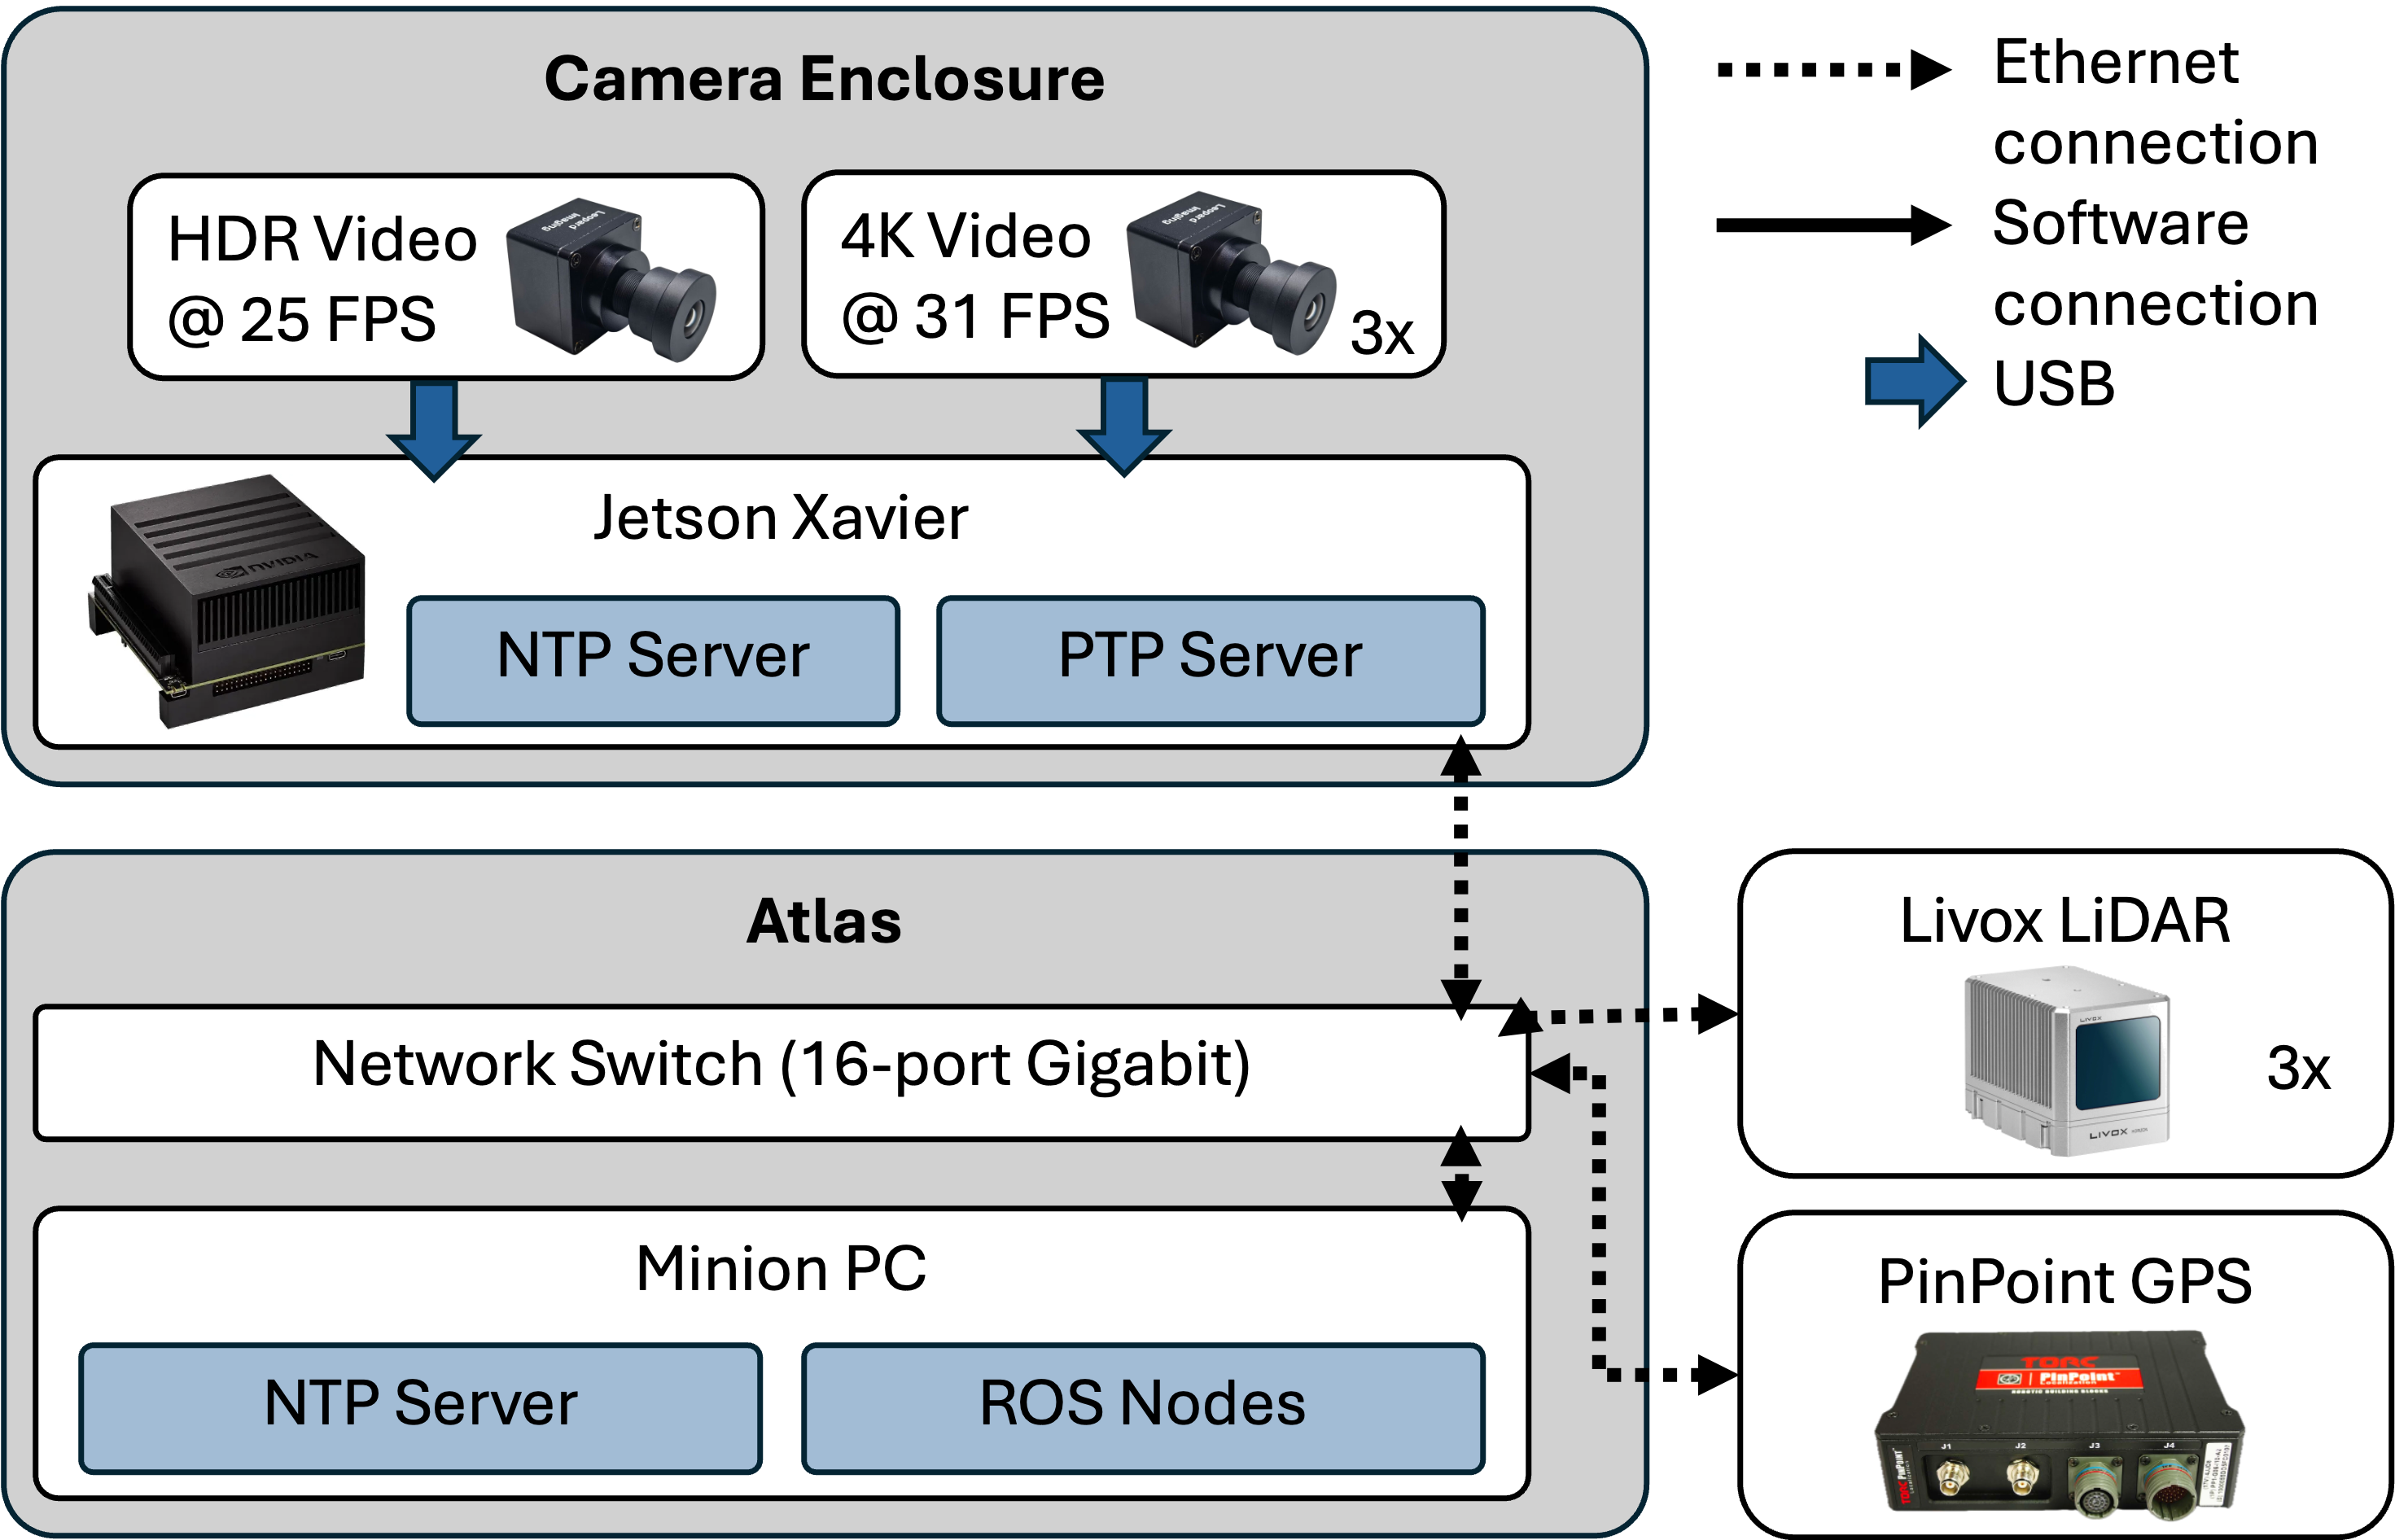
\includegraphics[width=0.8\textwidth]{Images/network_diagram2.png}
% \caption{Minion's LAN for network end-points related to real-time object detection}
% \label{fig:network_sync}
% \end{figure}

% The Jetson Xavier, serving as the core perception node, then acts as the PTP master for the Livox LiDAR units. Through the Precision Time Protocol (IEEE 1588), the Jetson broadcasts high-precision timestamps to all connected LiDAR clients, achieving microsecond-level synchronization between video and LiDAR data streams. This configuration ensures that every sensor measurement—image frame, LiDAR scan, or GPS fix—is temporally aligned to a common reference frame, enabling accurate data fusion and calibration as described in Section \ref{time_sync_cam}.

% Network bandwidth allocation is carefully managed to prevent congestion during real-time operation.
% Each Jetson video stream dynamically adjusts its bitrate based on the active frame rate, while LiDAR and telemetry traffic maintain constant low-latency channels.
% Table \ref{table:network_bandwidth} summarizes the approximate bandwidth usage across major network components.

% \begin{table}[htbp]
% \centering
% \begin{tabular}{lcc}
% \hline
% \textbf{Data Source} & \textbf{Protocol / Port} & \textbf{Typical Bandwidth (Mbps)} \\
% \hline
% HDR Camera Stream (Jetson $\rightarrow$ Atlas) & RTP / UDP & 3.7–11.2 \\
% FLIR Camera Streams (2x) & RTP / UDP & 7.0–20.0 (total) \\
% Livox LiDAR Units (3x) & UDP / PTP Client & 15.0–18.0 (total) \\
% GPS / INS Telemetry & NMEA / TCP & $< 0.1$ \\
% PTP Synchronization Packets & IEEE 1588 / UDP & $< 0.01 $\\
% \hline
% \textbf{Total Estimated Utilization} & — & \textbf{25–50 Mbp/s} \\
% \hline
% \end{tabular}
% \caption{Approximate Network Bandwidth Utilization}
% \label{table:network_bandwidth}
% \end{table}

% Security considerations for remote access include firewall configuration to restrict inbound connections, authentication requirements for SSH administrative access, and potential disconnection of external network access during sensitive operations to prevent unauthorized interference. The remote access infrastructure facilitates collaboration between multiple researchers working on different system components, as well as monitoring by shore-based personnel during extended autonomous operations.

% \subsubsection{Integration with Distributed Computing Architecture}

% The network infrastructure provides the physical medium for the distributed computing architecture that spans multiple platforms. The Jetson Xavier camera enclosure performs video encoding at the sensor location, transmitting compressed streams to the Atlas PC for object detection processing. This distribution optimizes bandwidth utilization by avoiding transmission of raw uncompressed video while maintaining centralized processing for computationally intensive algorithms.



% \subsubsection{Network Performance Validation}

% Network performance validation procedures employed during system commissioning verify that the infrastructure meets requirements for real-time perception and control. These procedures include bandwidth testing using iperf3 or similar tools to verify Gigabit link speeds between key endpoints, latency measurement via ping utilities to measure round-trip latency for time-critical paths, packet loss assessment through extended ping tests or UDP stream analysis to verify zero packet loss under load, and time synchronization quality monitoring to confirm clock accuracy meets requirements as detailed in Section \ref{time_sync_lan}.

% These validation procedures ensure that the network infrastructure meets the performance requirements necessary for real-time multi-modal perception and accurate temporal alignment of sensor data. Baseline performance metrics established during commissioning provide reference values for ongoing network health monitoring during field operations.

%%%%%%%%%%%%%%%%%%%%%%%%%%%%%%%%%%%%%%%%%%%%%%%%%%%%%%%%%%%%%%%%%%%%
%%%%%%%%%%%%%%%%%%%%%%%%%%%%%%%%%%%%%%%%%%%%%%%%%%%%%%%%%%%%%%%%%%%%
% \section{Sensor Calibration} \label{sec:calibration}

% The multi-sensor perception suite described in the previous section integrates complementary sensing modalities: \ac{LiDAR} for spatial structure and cameras for visual context.
% Each of these sensors measures the environment within its own reference frame and according to its own internal clock.
% To combine their observations into a consistent world model, the system must first be calibrated both spatially and temporally.

% Spatial calibration establishes the geometric relationships among all sensing elements.
% It quantifies each sensor’s intrinsic parameters—those governing the internal projection or ranging model—and the extrinsic transformations that define their relative positions and orientations within the overall platform.
% In the context of this work, the global chain of spatial relationships is implemented in the \ac{ROS} \texttt{tf\_tree}, linking coordinate frames from the \ac{GPS} and inertial reference through each \ac{LiDAR} unit to the visible-spectrum cameras.
% Accurate spatial calibration ensures that a point detected in a \ac{LiDAR} scan can be correctly projected onto the image plane, enabling correspondence between geometric and visual detections for downstream fusion.

% Temporal calibration aligns sensor data streams in time, ensuring that observations correspond to the same physical instant.
% Because each device maintains its own internal clock and sampling rate—\ac{LiDAR} operating at 100Hz with microsecond timestamps and cameras capturing 10Hz video with millisecond precision—even small timing offsets can lead to significant spatial error.
% % For a vessel traveling at 5 m/s, a 100ms misalignment translates to roughly 0.5~m of positional discrepancy between sensor modalities.
% To mitigate this, a sensor and system clocks are synchronized to the master GPS-disciplined time signature using \ac{NTP} and \ac{PTP} methods.
% Video timestamps allow temporal drift to be measured and corrected for high-precision multi-modal object detection.

% Spatial calibration methods, including camera intrinsic and extrinsic estimation and multi-\ac{LiDAR} registration, are presented in Section \ref{spatial_calibration}, followed by the temporal synchronization framework in Section~\ref{time_sync}.
% Each section details both the methods employed and the resulting calibration accuracy achieved.
% % brief overview of TF_tree

% %%%%%%%%%%%%%%%%%%%%%%%%%%%%%%%%%%%%%%%%%%%%%%%%%%%%%%%%%%%%%%%%%%%%
% %%%%%%%%%%%%%%%%%%%%%%%%%%%%%%%%%%%%%%%%%%%%%%%%%%%%%%%%%%%%%%%%%%%%

% %%%%%%%%%%%%%%%%%%%%%%%%%%%%%%%%%%%%%%%%%%%%%%%%%%%%%%%%%%%%%%%%%%%%
% \subsection{Spatial Calibration} \label{spatial_calibration}

% % # Spatial Calibration

% Before the data from the camera and \ac{LiDAR} sensors can be combined, each device needs to be spatially calibrated through extrinsic and intrinsic transforms.
% Every sensor measures the environment relative to its own local coordinate frame.
% Minion uses a forward-left-up (FLU) reference frame to express its position and orientation within the inertial map frame, and the data from each sensor must undergo a rotation and translation to create a unified perception model.

% Intrinsic calibration characterizes the internal geometric and optical properties of each camera, quantifying lens distortion, focal length, principal point location, and sensor pixel geometry.
% Extrinsic calibration determines the six-degree-of-freedom transformation required to translate one reference frame into another.

% The sensor transforms required to move between the sensors specific to Minion are presented as a transform tree in Figure \ref{fig:tf_tree}. 
% The port and starboard Livox points undergo extrinsic transforms into the center Livox frame before being combined into a unified point cloud.
% To project LiDAR points from the center Livox into the HDR camera frame, these three-dimensional X-Y-Z points are transformed through the extrinsic transform between the two sensors, followed by transformation according to the camera's intrinsic transform into the two-dimensional X-Y pixel values required to place them in the image frame.
% All sensor data undergoes two transforms to be placed onto the map frame, first through the GPS frame, which defines Minion's origin and orientation, and finally to the inertial Map frame.

% Combined, these calibrations enable observations between sensor coordinate systems, projection of \ac{LiDAR} points onto camera images, and registration of multi-modal sensor data for fusion applications.

% \begin{figure}
%     \centering
%     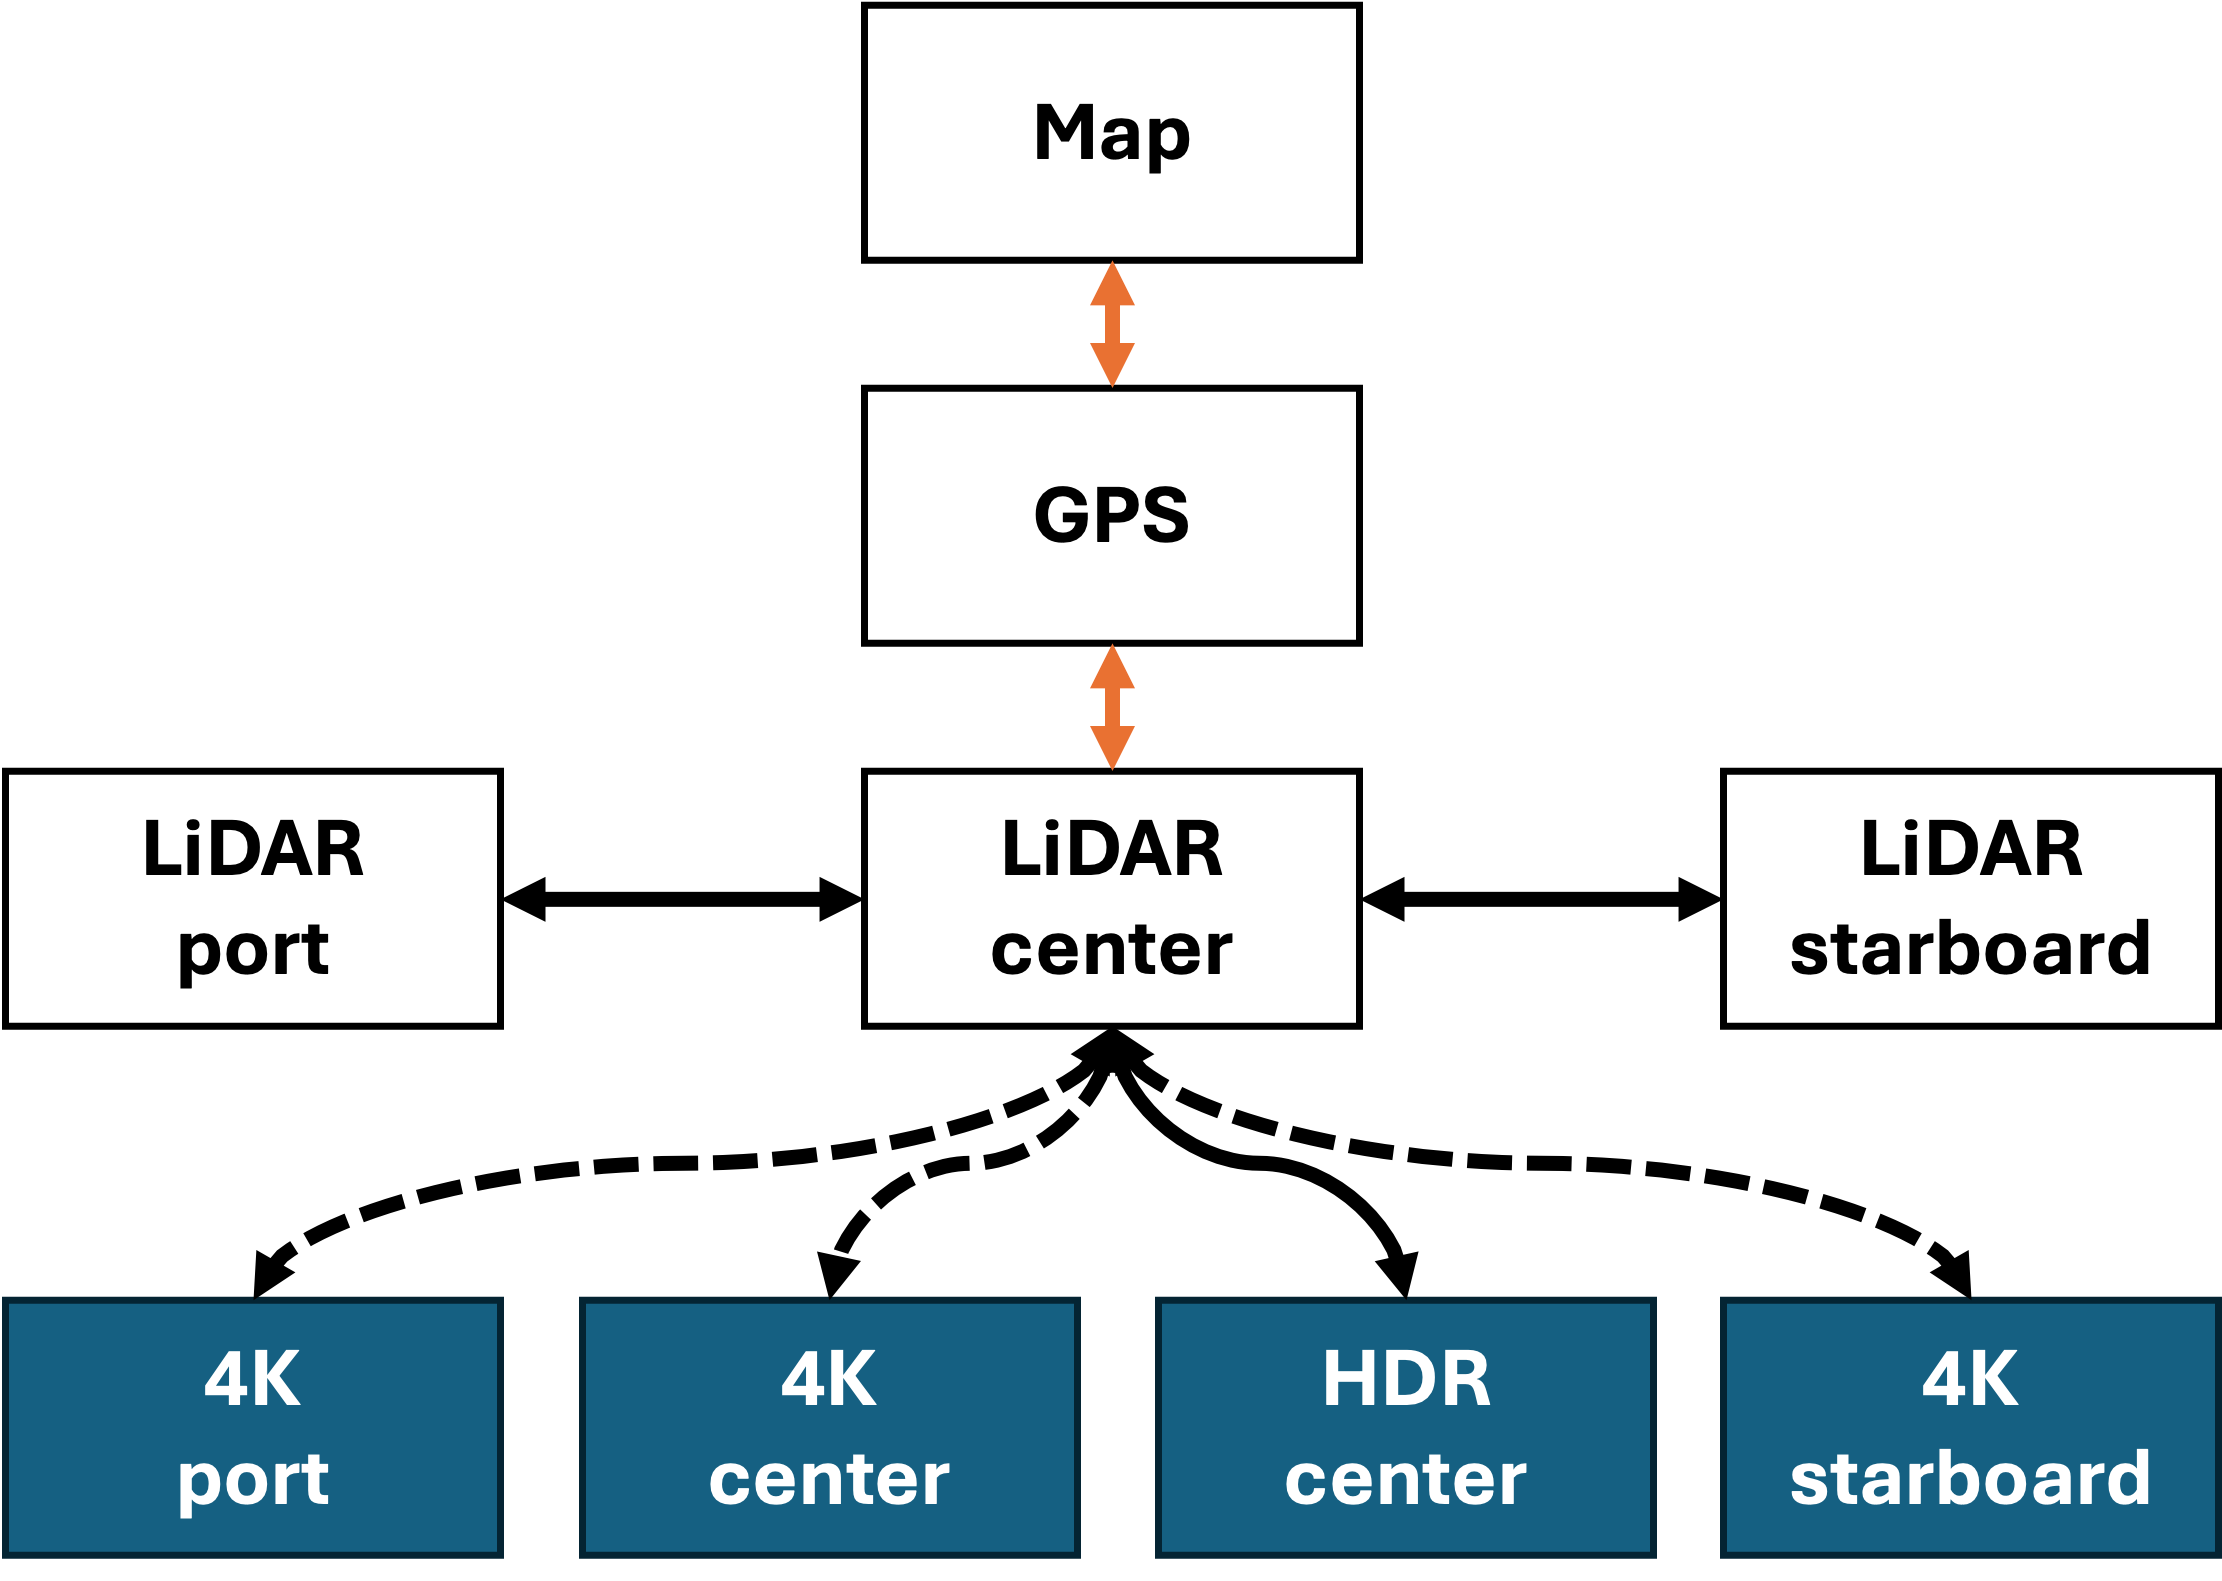
\includegraphics[width=0.7\linewidth]{Images/tf_tree.png}
%     \caption{Spatial transform tree between sensor reference frames onboard Minion.}
%     \label{fig:tf_tree}
% \end{figure}

% Because these transforms stack upon each other, they require calibration to achieve a level of precision to minimize compounding errors through the tree.
% Additionally, each sensor must maintain precise relative timing to one another to align the data from each sensor temporally.

% This section discusses the methods used to define these spatial transformations in \ref{spatial_calibration}, as well as temporal synchronization in \ref{time_sync}.

% \subsubsection{Camera Intrinsic Calibration} \label{HDR_intrinsic}

% Camera intrinsic parameters describe the internal geometry of a camera and define the mapping between three-dimensional coordinates in the camera frame and two-dimensional pixel locations in the image plane.  



% \subsubsection{Workload Allocation}

% The CPU-GPU task distribution reflects algorithm characteristics and hardware capabilities.
% LiDAR processing with irregular spatial queries and dynamic data structures exploits CPU cache hierarchies and branch prediction, while vision processing with regular tensor operations and data parallelism leverages GPU throughput.
% The 6-core CPU handles approximately 3× simultaneous LiDAR processing streams plus sensor fusion logic without saturating computational resources, while the 2560-core GPU processes vision workloads that would overwhelm CPU execution.

% This balanced allocation maintains real-time performance with sub-100 millisecond end-to-end latency from sensor observation to fused detection output, meeting the temporal requirements for autonomous navigation decision-making.
% Load monitoring during typical operations indicates approximately 60-70\% CPU utilization across all cores and 70-80\% GPU utilization during simultaneous LiDAR and vision processing, providing margin for computational bursts during high-complexity scenes.

% % \paragraph{CPU-Based Processing}

% LiDAR point cloud processing and LiDAR-based object detection are executed on the system’s multi-core CPU.
% These algorithms involve spatial clustering, coordinate transformations, and probabilistic data association—operations that rely on irregular memory access patterns and branching logic.
% Such workloads benefit from the CPU’s high single-threaded performance, cache hierarchy, and flexible memory management.
% The CPU also performs sensor fusion between LiDAR and vision detections, as well as general system coordination tasks such as recording data. %, network management, and operator interface control.

% % \paragraph{GPU-Based Processing}

% The GPU accelerates two perception tasks that exhibit a high degree of data parallelism: video decoding and deep learning inference.
% Its first responsibility is processing video streams received from the camera enclosure. 
% Video decoding and image preprocessing are performed directly in GPU memory, minimizing data transfer overhead and reducing end-to-end latency.
% The second responsibility is image-based object detection using the \ac{YOLO} framework. 
% This algorithm relies on convolutional and tensor operations within neural networks and is implemented to leverage the parallel processing capabilities of NVIDIA’s CUDA architecture.

% \subsubsection{Storage Media}

% and 5–15MBps per camera for H.265-compressed video at 10~fps, with additional low-bandwidth streams for GPS/INS and detection results.
% The NVMe solid-state drives provide sufficient sequential throughput and IOPS to maintain these rates for extended sessions without frame loss or buffer overflow.

% \textcolor{red}{If time allows, it may be worth mentioning the cooling system.}

% \subsubsection{GPU}

% The NVIDIA GTX~1080 GPU accelerates the vision-based object detection pipeline by handling tasks that benefit from highly parallel computation.  
% Its primary responsibilities include decoding the incoming video streams from the camera enclosure and performing the image convolution operations required for vision-based detection.  
% The GPUs have hardware-accelerated video encoders and decoders for processing multiple video streams, and an object-detection algorithm was written to leverage the 2,560 CUDA cores for fast tensor and matrix computations and image convolution.
% This also offloads H.264 decompression from the CPU, allowing the system to process multiple high-resolution camera streams simultaneously while preserving CPU resources for LiDAR and sensor-fusion tasks.

  
% These operations are executed directly in GPU memory, leveraging  cores  the repetitive tensor and matrix computations common to neural network inference.  
% This hardware acceleration enables real-time image processing and object detection performance that would otherwise be infeasible on CPU resources alone.

% Each GTX 1080 GPU features 2560 CUDA cores based on NVIDIA's Pascal architecture with 8 GB of GDDR5X memory, accelerating both machine learning inference for object detection video decoding tasks.
% The Pascal architecture provides CUDA compute capability 6.1, enabling efficient execution of YOLOv8 convolutional neural networks and GPU-accelerated image preprocessing described in Chapter \ref{realtime_object_detection}.
% Hardware video decode engines offload H.264 video decompression from the CPU, enabling the Atlas PC to receive and process multiple camera streams simultaneously while maintaining CPU resources for perception algorithms.

% \subsubsection{GPU}

%% Atlas

% Minion A was configured with Ubuntu 22.04 for the development and migration of Minion's software to ROS 2 Humble, while 
% Minion B served as the only device used for data-recording and object-detection processing performed for the research of this dissertation, and ran Ubuntu 20.04 with ROS 1 Noetic.

% While ROS manages sensor data and transforms between reference frames, the focus in this section relates to the underlying hardware responsible for real-time, multi-modal perception.  
% The object-detection methods described in Chapter \ref{realtime_object_detection} are optimized for the computational characteristics of the CPU and GPU.  
% This distribution of processing responsibilities balances throughput, latency, and efficiency across the perception pipeline.  
% The following subsections describe how LiDAR and vision workloads are allocated between the CPU and GPU on the Atlas platform.

% While the ROS middleware manages communication and synchronization between sensor nodes, the emphasis here is on the computational workload executed by the Atlas hardware. 

% Perception processing is divided between CPU and GPU resources according to the characteristics of each object detection method.  
% LiDAR-based object detection, is performed on the CPU due to its reliance on irregular memory access patterns and control flow.  
% Conversely, vision-based detection utilizes parallel tensor operations that the GPU hardware is optimized for.  
% This allocation of workloads balances computational throughput and latency, ensuring reliable multi-modal perception and sensor fusion for autonomous operation.

% primarily between the CPU and GPU according to algorithm characteristics and hardware acceleration capabilities.

% have different workload requirements, and therefore operate primarily on separate processing units.
% Perception workloads are 
% This 
% While \ac{ROS} manages coordination and communication across processes, the following overview focuses on the hardware-level execution of LiDAR and vision tasks.

% \subsubsection{CPU and Memory}
% Each Atlas PC is equipped with computing hardware selected to meet the demanding real-time requirements of multimodal perception and autonomous operation.  
% % Table~\ref{table:Minion_hardware} summarizes the key system specifications.
% The Intel Xeon processor provides six cores and a total of twelve parallel threads for concurrent perception and navigation processes.
% Tasks that require low-latency responses—such as LiDAR point cloud filtering and sensor updates benefit from the processor’s strong single-thread performance.
% % , which minimizes delay between sensor input and system response.  
% At the same time, the multi-core architecture supports parallel execution of computationally intensive workloads.
% % , including feature extraction and classification across multiple LiDAR streams.  
% Hardware vector acceleration further enhances numerical operations common to point cloud transformations and coordinate frame calculations.

% The system’s 16~GB of high-bandwidth memory provides sufficient capacity to buffer LiDAR point clouds, video imagery, and other sensor data during real-time processing.  
% This configuration allows multiple perception modules to access and update shared data concurrently without slowing overall system performance.

% \subsubsection{CPU and Memory}


%%%%%%%%%%%%%%%%%
% camera enclosure

% Local recording also serves diagnostic purposes, enabling comparison of locally-saved video files with network-transmitted ROS bag data to validate timestamp accuracy and detect any frame dropping or duplication during network transmission. The temporal drift analysis methodology described in Section \ref{time_sync_cam} exploits this local recording capability by comparing locally-saved video frames with network-transmitted ROS messages to quantify systematic timing offsets introduced by the encoding-transmission-decoding pipeline.


% The video encoding workflow exploits the Jetson's dedicated hardware encoding engines to achieve real-time compression of three simultaneous 2880×1860 pixel video streams. Hardware encoding offloads the computationally intensive compression operations from the CPU, enabling sustainable operation without thermal throttling during extended recording sessions. The RTSP bitrate is [INSERT bitrate formula here] dependent upon the requested stream frame rate (typically 5-15 fps).

% The compressed video streams are transmitted to the Atlas PC main computing platform via RTSP over UDP, where they are decoded and published as ROS image messages for consumption by object detection algorithms. This architecture distributes the encoding burden to the camera enclosure while centralizing detection processing on the more powerful Atlas hardware.

% A critical function performed by the Jetson Xavier is the embedding of precise system timestamps directly into the encoded video bitstream. Custom GStreamer pipeline elements inject SEI (Supplemental Enhancement Information) NAL units containing synchronized timestamps alongside encoded video frames. This in-band metadata approach ensures that timing information persists with the video data through network transmission, recording, and playback. The temporal synchronization procedures and timestamp validation methodology are detailed in Section \ref{time_sync_cam}.

% \subsubsection{Network Infrastructure Role}

% Within Minion's distributed computing architecture, the Jetson Xavier subscribes to the precise GPS clock provided by the Pinpoint.

% erves several network infrastructure functions. As described in Section \ref{time_sync_lan}, the system participates 

% in the hierarchical time distribution network that provides temporal synchronization for all platform sensors. The Jetson operates as both a client for receiving GPS-disciplined time and a server for providing high-precision timing to the LiDAR sensors.

% The Gigabit Ethernet interface connects the camera enclosure to the vessel local area network at IP address 201.7.90.147. This single network connection carries bidirectional traffic including compressed video streams, time synchronization protocols, remote administration access, and platform status monitoring. The camera enclosure may also include a secondary Ethernet switch to provide local network connectivity for the three Livox Horizon LiDAR units mounted on or near the camera mast, as detailed in Section \ref{comp:camera_enclosure}.

% \subsubsection{Local Recording Capability}


% Each camera stream defaults to 5 \ac{fps} to match the data rate of other perception data, but can be modified based upon need.
% This  us a default maintaining each stream below 25–30 Mbps to prevent network saturation.
% This ensures bandwidth allocation per stream remains within network limits while preserving visual fidelity.

% ## NVIDIA Jetson Xavier Platform
% The Jetson Xavier’s 8-core ARM processor provides ample computational capacity for managing multiple video pipelines, network protocols, and system services, while the integrated 512-core Volta GPU enables hardware-accelerated video encoding required for concurrent high-resolution stream processing.  
% A shared 32~GB pool of unified memory between the CPU and GPU supports high-throughput data exchange, ensuring efficient media handling and minimizing latency within the video processing pipeline.

% % \subsubsection{Video Processing Architecture}
% The primary computational responsibility of the Jetson Xavier is video encoding and transmission of video from the six cameras.
% % three 4K cameras, two FLIR, and a single HDR camera feeds. 
% The pipeline for each video follows a similar structure: raw video frames are received via USB 3.0, parsed by custom software, and then split into two processing branches. 
% One branch is encoded in H.265 and saved locally to the Jetson's internal storage, while the other branch is down-sampled to a reduced frame rate before being streamed over the \ac{LAN} to one of the Minion PCs in Atlas.


% # Camera Enclosure Computing Platform

% for the RobotX competition in 2022, as well as the PhD research of D. Thompson \cite{thompson2023}.
% Specialized computing hardware is required to manage up to six video streams from the cameras within the enclosure.
% The camera enclosure assembly integrates six camera sensors with dedicated computing hardware housed in a weatherproof enclosure mounted on the vessel's superstructure. 


% real-time H.264/H.265 video encoding, manages timestamp embedding for temporal synchronization, and serves critical time distribution functions within the hierarchical clock architecture. This distributed computing approach places video processing at the camera location rather than transmitting raw uncompressed video over the network, substantially reducing bandwidth requirements while enabling sophisticated in-stream timestamp embedding.

% The camera enclosure houses six cameras and serves as the mount for the three forward Livox LiDAR units, and was designed to be a self-contained perception platform for any maritime vessel or ground vehicle. 
The camera enclosure serves as the integrated perception module for the vessel, and was designed as a self-contained sensor and computing subsystem that can operate independently on any maritime or ground vehicle. 
Integrated into this subsystem is a NVIDIA Jetson AGX Xavier, a compact and capable PC designed for video processing, as well as other computer vision applications.
% The system-on-module (SOM) design combines ARM-based CPU cores with a powerful GPU architecture optimized for media encoding and AI tasks. 
% The system-on-module (SOM) design integrates a processor, GPU, and memory in a compact form factor designed for speed and power efficiency.
Key hardware specifications are provided in table \ref{table:Xavier_hardware}.
% The Jetson AGX Xavier serves as the dedicated processing unit within the camera enclosure, managing video acquisition, compression, and transmission from all six cameras.  

Its 8-core ARM processor provides ample computational capacity for handling multiple video pipelines, network protocols, and system-level services, while the integrated 512-core Volta GPU performs hardware-accelerated video encoding required for concurrent high-resolution streams.  
A unified memory architecture shares 32 GB between the CPU and GPU and supports a memory bandwidth of 136.5 GBps, which minimizes latency and improves overall pipeline efficiency.

Each video feed follows a two-branch processing pipeline before being transmitted to Atlas.  
% Raw frames are captured over USB~3.0 and parsed by custom software before being distributed to parallel encoding tasks. 
Raw video frames are received via USB 3.0, parsed by custom software, and then split into two processing branches. 
One branch is compressed and saved locally to the Jetson's internal storage, while the other branch is down-sampled to a reduced frame rate before being streamed over the \ac{LAN}.% to one of the Minion PCs in Atlas.


%% compute/lan

% The device interfaces with the vessel's compute infrastructure via Ethernet, configured at IP address 201.7.90.30 on the local network.
% Beyond navigation, the Pinpoint unit serves dual roles: providing a high-accuracy time reference for sensor synchronization and delivering six-degree-of-freedom pose estimates through onboard sensor fusion algorithms.
% The specific methodologies for temporal calibration and synchronization using this device are detailed in Section 3.2.2.1, while the spatial calibration procedures appear in Section 3.2.3.


% Global Navigation Satellite System signals inherently carry highly accurate timing information, as satellite positioning operates through precise measurement of signal delay from multiple satellites with synchronized atomic clocks.
% The PinPoint receiver extracts this timing information and distributes it over the vessel's network using Network Time Protocol.
% The \ac{GPS} unit was assigned a static IP address of 201.7.90.30 on the Minion network and configured to broadcast \ac{GPS}-disciplined time via Network Time Protocol.
% The Atlas PC main computer synchronizes its clock to this \ac{GPS} source with typical accuracy in the tens to hundreds of nanoseconds, limited primarily by network latency rather than \ac{GPS} accuracy.

% This \ac{GPS} time reference propagates through the synchronization hierarchy to every computing resource on the platform.
% Atlas functions as a Network Time Protocol server for the NVIDIA Jetson Xavier camera computer, which subsequently operates as a Precision Time Protocol master for the Livox Horizon \ac{LiDAR} sensors.
% This cascaded approach ensures timestamps from all sensors—cameras, \ac{LiDAR}, and \ac{GPS}/\ac{IMU}—share a common time reference traceable to \ac{GPS} time.

% Beyond timekeeping, the \ac{GPS}/\ac{IMU} system continuously tracks platform position and orientation, which is required for \ac{LiDAR} temporal aggregation.
% As described in Section 3.1.1.3, accumulating \ac{LiDAR} points over several seconds necessitates compensation for vessel motion during that period.
% The PinPoint system fuses \ac{GPS} position measurements with \ac{IMU} acceleration and rotation data through an Extended Kalman Filter to produce pose estimates at rates substantially higher than \ac{GPS} alone could provide.
% \ac{GPS} fixes arrive at 1-10 Hz depending on satellite visibility, while the \ac{IMU} operates at hundreds of hertz.
% The fusion algorithm propagates pose estimates forward using \ac{IMU} integration between \ac{GPS} updates, subsequently correcting accumulated drift when new \ac{GPS} measurements arrive.

% The resulting pose solution provides six-degree-of-freedom state estimates—three-dimensional position and three-dimensional orientation—at sufficient temporal resolution to interpolate platform pose to the exact timestamp of each \ac{LiDAR} point.
% This capability supports the transformation methodology presented in Chapter 5, where \ac{LiDAR} points acquired at different times during motion are transformed to a common reference frame before projection onto camera images.

% The PinPoint \ac{GPS}/\ac{IMU} connects to the Minion computing infrastructure via Ethernet, utilizing both Network Time Protocol for time distribution and User Datagram Protocol for pose data transmission.
% \ac{ROS} driver nodes on the Atlas PC receive and parse the binary \ac{GPS}/\ac{IMU} messages, publishing pose estimates as standard \ac{ROS} geometry messages.
% These messages incorporate position (latitude, longitude, altitude), orientation (roll, pitch, yaw), uncertainty estimates, and \ac{GPS} fix quality flags.
% The \ac{ROS} tf2 library consumes these pose estimates to maintain the time-varying transformation tree relating sensor frames to platform and world frames, enabling automated coordinate transformation for sensor fusion.

% The \ac{GPS}/\ac{IMU} defines the local reference frame for the platform \texttt{base\_link}, with position expressed in geographic coordinates (WGS84 datum) and orientation relative to true north and local gravity.
% This world-referenced system serves as the common reference for transforming observations from multiple sensors acquired at different times during motion.
% Transformation from sensor-local frames to the \ac{GPS}/\ac{IMU} world frame requires knowledge of sensor-to-platform extrinsic calibration parameters.
% These parameters are determined through calibration procedures described in Section 3.2.1.2 for cameras and Section 3.2.1.3 for \ac{LiDAR} sensors.
% With extrinsic parameters established, the \ac{GPS}/\ac{IMU} pose solution enables transformation of any sensor observation to world coordinates or to any other sensor's reference frame.

% Maritime environments present challenges for \ac{GPS}/\ac{IMU} systems that differ from land vehicle applications.
% Water surface reflections induce multipath interference in \ac{GPS} signals, while vessel pitch and roll motion exercises the full range of the \ac{IMU}.
% The PinPoint system was designed for marine applications and incorporates algorithms to address these factors while maintaining accuracy during vessel maneuvering.
% \ac{GPS} accuracy degrades in areas with limited satellite visibility, such as proximity to tall structures, bridges, or fjord-like coastal terrain.
% The \ac{IMU} provides short-term pose continuity during \ac{GPS} outages, though accumulated drift limits the duration for which pure inertial navigation remains accurate.
% Data collection operations were conducted in open water with favorable satellite visibility, ensuring consistent \ac{GPS} fix quality throughout recording sessions.

% The \ac{GPS}/\ac{IMU} system enables two functions essential for multi-modal sensor fusion research.
% First, \ac{GPS}-disciplined time distributed to all sensors ensures timestamps from cameras, \ac{LiDAR}, and \ac{GPS} itself reference the same time base, providing frame-accurate temporal association across modalities.
% Second, continuous pose estimates enable transformation of temporally distributed observations to common reference frames, supporting \ac{LiDAR} aggregation during motion and registration of sensor fields of view for fusion operations.
% Combined with the synchronization verification and drift correction procedures described in Section 3.2.2, these capabilities establish the temporal and spatial foundation for rigorous object detection performance evaluation across sensing modalities.
% The \ac{GPS}/\ac{IMU} thus functions not merely as a navigation sensor but as critical infrastructure enabling the multi-modal perception analysis central to this research.

%% Camera Selection


% This performance is enabled by a digital overlap \ac{HDR} (DOL-HDR) architecture with in-pixel dual conversion gain.  
% By capturing multiple gain levels within a single frame period, the sensor produces simultaneous multi-gain readouts without relying on sequential multi-exposure stacking.  
% This design eliminates ghosting and motion artifacts, which are common when either the platform or surrounding targets move between exposures.  

% \subsubsection{Leopard Imaging HDR Camera}

% To overcome these limitations, a \ac{HDR} camera from Leopard Imaging was integrated, based on Sony’s IMX490 automotive-grade \ac{HDR} sensor.  
% This camera provides 65 degrees of forward coverage and achieves approximately 120~dB of dynamic range, enabling preservation of fine image details across extreme lighting conditions, including bright sky, reflective water, and shaded objects.  



% This substantial increase in dynamic range, combined with robust performance under challenging illumination, made the IMX490-based \ac{HDR} camera the primary visual spectrum sensor for \ac{LiDAR}-camera fusion research in this dissertation.  
% Preliminary results from a comparative study by Liebergall et al.~\cite{liebergall} further supported this decision, showing improved detection consistency with the \ac{HDR} sensor compared to the FLIR 4K cameras.  
% Although later published results did not fully corroborate the preliminary findings, those results became available only after the dataset for this research had been collected.  
% Accordingly, the IMX490 \ac{HDR} camera served as the main forward-facing visual spectrum sensor throughout this study.  



% The 2880×1860 resolution provides sufficient spatial detail for detecting objects at relevant ranges in autonomous vessel navigation, while the 25 fps frame rate adequately supports typical vessel speeds and maneuvering.

% The IMX490's native \ac{HDR} combines multiple exposures in a single frame period, achieving 120 dB dynamic range without sequential multi-exposure capture.
% This simultaneous approach eliminates motion artifacts associated with temporal bracketing, which is critical when both the platform and targets are in motion.
% Image quality validation and intrinsic calibration are addressed in Section 3.2.1.1, including lens distortion characterization and camera matrix estimation.
% The combination of wide dynamic range, moderate resolution, and calibrated geometry provides the image quality necessary for training and evaluating vision-based detection models in Chapter 5.

% Thompson et al. \cite{thompson2023} originally developed this camera hardware and integration approach, establishing a foundation for maritime perception research.
% The primary enhancement introduced in this work comprises in-band timestamp embedding and temporal drift correction, detailed in Section 3.2.2, which are essential for rigorous multi-modal sensor fusion analysis.


%%%%%% image resolution



% Insert equation to get the horizontal focal length / horizontal resolution ratio needed for camera selection based upon the equation and information provided above
% Assuming our camera will have a landscape aspect ratio, our equation becomes 
% Since the detection network downsamples each input frame to a maximum dimension of 640 pixels while preserving aspect ratio, a landscape-oriented image with native resolution $N_x \times N_y$ (where $N_x > N_y$) is scaled such that the horizontal dimension becomes 640 pixels.
% For an object that must occupy at least $w_{\text{net}}$ pixels horizontally in the network input to be reliably detected, the camera system must satisfy
%   \begin{equation}
%   \frac{f}{S_w} = \frac{w_{\text{net}} \, d}{640 \, W}
%   \end{equation}
% \begin{equation}
%  w_{\text{px}} \left(\frac{650}{N_x}\right) = f \; \frac{N_x}{S_w}\frac{W}{d}
% \end{equation}

% where the ratio $f/S_w$ represents the normalized focal length of the camera-lens system.
% Substituting the minimum object dimensions ($W = 0.3683$ m, $d = 60$ m) and assuming a minimum network resolution requirement of $w_{\text{net}}$ pixels, this relationship defines the optical design space for camera selection.
% This makes our equation

% \begin{equation}
% w_{\text{px}} = \frac{f \, N_x^2 \, W}{(680)S_w \, d}
% \end{equation}


%%%%%%%%% Livox



%%%%%%% move to sensor calibration %%%%%%%%%%%
% Accurate fusion of data from multiple \ac{LiDAR} units requires precise knowledge of sensor geometric relationships.
% The Livox Horizon units feature onboard storage for extrinsic calibration parameters, enabling each sensor to transform its measurements to a common reference frame before transmission.
% These parameters are written to non-volatile memory on each Livox unit and applied before data transmission so that all LiDAR returns are received in the center \ac{LiDAR}'s reference frame, reducing the necessary calculation further down the data pipeline.
% \textcolor{red}{cite Livox documentation?}.
% enhancing their real-time operational advantage by reducing additional computation later in the pipeline.
% The calibration methodology to determine these extrinsic values is detailed in Section~\ref{LiDAR_extrinsic}.
%%%%%%%%%%%%%%%%%%%%%%%%%%%%%%%%%%%%%%%%%%%%%%%

% The 905 nm near-infrared wavelength experiences strong absorption by water, resulting in minimal returns from water surfaces.
% This characteristic benefits maritime object detection by reducing clutter from waves that would otherwise trigger false positives in clustering algorithms.

% The fundamental distinction between the Livox Horizon and traditional spinning \ac{LiDAR} lies in the scan pattern.
% A mechanically spinning sensor with N lasers produces N discrete horizontal rings that repeat identically each rotation.
% For vessels moving at typical speeds (2-5 m/s), platform displacement between rotations remains small relative to object size, resulting in near-perfect overlap of consecutive scans.
% The Livox operates differently, employing a two-dimensional scanning mechanism that traces a non-repetitive rosette pattern across the \ac{FOV}.
% Two orthogonal mirrors operating at slightly different frequencies cause the laser beam to trace a complex Lissajous-like path that progressively fills the \ac{FOV} without repetition \cite{thompson2023}.

% Scan pattern coverage accumulates over time, with longer integration periods yielding denser spatial sampling.
% At the standard 100 Hz output rate, each \ac{UDP} message contains approximately 10 milliseconds of returns.
% Over a one-second aggregation period, the rosette pattern provides substantially higher spatial coverage than a spinning sensor's fixed ring geometry.

% The non-repetitive forward-scanning nature of the Livox units means that point cloud density is not uniform across the \ac{FOV}.
% The 81.7-degree horizontal \ac{FOV} allows for overlap between the three units, achieving more uniform density across the 165-degree \ac{FOV}, matching the 4K FLIR camera coverage.

% Insert figure showing Livox scan pattern here
% \begin{figure}[htbp]
% \centering
% 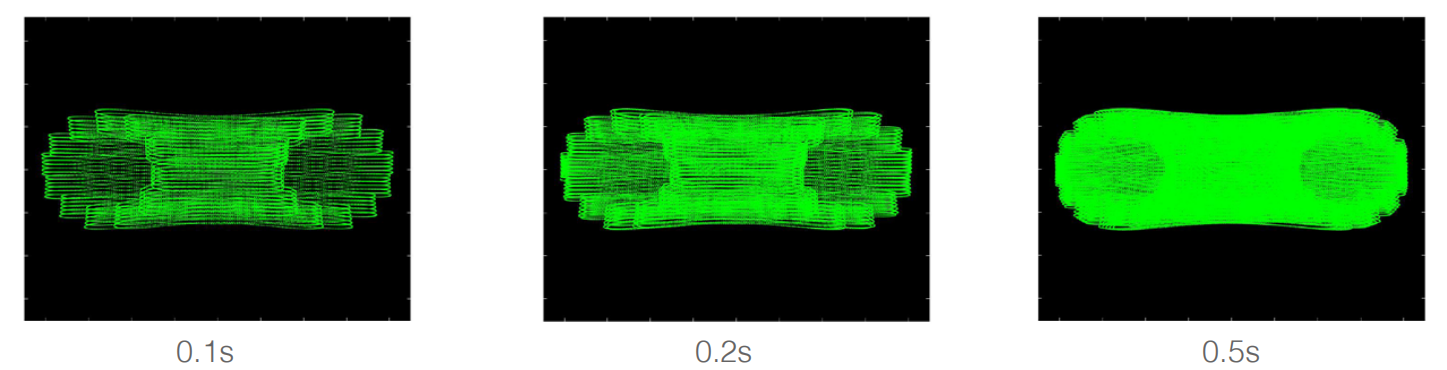
\includegraphics[width=0.8\textwidth]{Images/Livox_1.png}
% \caption{Livox Horizon non-repetitive rosette scan pattern demonstrating point cloud density distribution from 0.1 to 0.5 seconds.}
% \label{fig:livox_scan_pattern}
% \end{figure}




% A Velodyne VLP-16 in dual-return mode produces approximately 1.4 million \ac{pps} distributed across the full 360-degree plane.
% The camera \ac{FOV} encompasses approximately 165 degrees, yielding an effective point rate in the region of interest of:

% $$\text{Effective HDL-32E rate} = 1.4 \times 10^6 \times \frac{165 degree}{360 degree} \approx 641,000 \text{ pts/sec}$$

% Three Livox Horizon units in dual-return mode together produce:

% $$\text{Combined Livox rate} = 3 \times 480,000 = 1.44 \times 10^6 \text{ pts/sec}$$

% This represents a 2.25× increase in point returns within the camera view, excluding additional benefits from superior vertical sampling achieved through the non-repetitive pattern compared to fixed 32-ring geometry \cite{thompson2023}.
